
%%%%%%%%%%%%%%%%%%%%%%%%%%%%%%%%%%%%%%%%%%%%%%%%%%%%%%%%%%%%%%%
%
%     filename  = "thesis.tex",
%     date      = "01/08/2009",
%     authors   = "Charles-Philippe Lajoie",
%     copyright = "Charles-Philippe Lajoie",
%     address   = "Physics & Astronomy,
%                  ABB,
%                  McMaster University,
%                  Hamilton, ON,
%                  CANADA",
%     telephone = "905-525-9140 ext.26057",
%     email     = "lajoiec@mcmaster.ca",
%
%%%%%%%%%%%%%%%%%%%%%%%%%%%%%%%%%%%%%%%%%%%%%%%%%%%%%%%%%%%%%%%


%\documentclass[twoside,phd]{macthesis}
\documentclass[twoside,letterpaper,phd]{macthesis}
%%%%%%%%%%%%%%%%%%%%%%%%%%%%
% Packages we like to use. %
%%%%%%%%%%%%%%%%%%%%%%%%%%%%
\usepackage{fancyhdr}
\pagestyle{fancy}
\usepackage{deluxetable}
\usepackage{natbib} % \citet,\citep
\usepackage{aastex_hack} % Taken from: http://casa.colorado.edu/~danforth/comp/tex/thesistex.html
\usepackage{rotating}

\usepackage{amsmath}
\usepackage{amssymb}
\usepackage{amsthm}
\usepackage{exscale}
\usepackage[mathscr]{eucal}
\usepackage{bm}
\usepackage{eqlist} % Makes for a nice list of symbols.

%\usepackage[final]{graphicx}

\usepackage{epigraph}
\usepackage{lettrine}
\usepackage{keyval}

\usepackage[dvipsnames]{color}
%\usepackage{times}
%\documentstyle[fancyhdr]
%\usepackage{tabular}
%\DeclareGraphicsExtensions{.pdf, .jpg}


\usepackage{multirow}

%%%%%%%%%%%%%%%%%%%%%%%%
% Setting for fncychap %
%%%%%%%%%%%%%%%%%%%%%%%%
% Comment out or remove the next two lines and you will get
% the standard LaTeX chapter titles. We like these A LOT
% better.
\usepackage[Lenny]{fncychap}
\ChTitleVar{\Huge\sffamily\bfseries}


%%%%%%%%%%%%%%%%%%%%%%%%%%%%%%%%%%%%
% SPECIAL SYMBOLS AND NEW COMMANDS %
%%%%%%%%%%%%%%%%%%%%%%%%%%%%%%%%%%%%
%\input{SupplementaryMaterial/UserDefinedCommands}


%%%%%%%%%%%%%%%%%%%%%%%%%%%%%%%%%%%%%%%%%
% Renewed Float Parameters              %
% (Makes floats fit better on the page) %
%%%%%%%%%%%%%%%%%%%%%%%%%%%%%%%%%%%%%%%%%
\renewcommand{\floatpagefraction}{0.85}
\renewcommand{\topfraction}      {0.85}
\renewcommand{\bottomfraction}   {0.85}
\renewcommand{\textfraction}     {0.15}



% Alter some LaTeX defaults for better treatment of figures:
% See p.105 of "TeX Unbound" for suggested values.
% See pp. 199-200 of Lamport's "LaTeX" book for detail
%   General parameters, for ALL pages:
\renewcommand{\topfraction}{0.9}	% max fraction of floats at top
\renewcommand{\bottomfraction}{0.8}	% max fraction of floats at bottom
%   Parameters for TEXT pages (not float pages):
\setcounter{topnumber}{2}
\setcounter{bottomnumber}{2}
\setcounter{totalnumber}{4}     % 2 may work better
\setcounter{dbltopnumber}{2}    % for 2-column pages
\renewcommand{\dbltopfraction}{0.9}	% fit big float above 2-col. text
\renewcommand{\textfraction}{0.07}	% allow minimal text w. figs
%   Parameters for FLOAT pages (not text pages):
\renewcommand{\floatpagefraction}{0.7}	% require fuller float pages
% N.B.: floatpagefraction MUST be less than topfraction !!
\renewcommand{\dblfloatpagefraction}{0.7}	% require fuller float pages

% ----------------------------------------------------------- %

%%%%%%%%%%%%%%%%
% FRONT-MATTER %
%%%%%%%%%%%%%%%%
% Title
\title{The Physics of Mergers:  Theoretical and Statistical Techniques \\
  Applied to Stellar Mergers in Dense Star Clusters}
% Author and Department
\author{Nathan W. C. Leigh}
\dept{Physics and Astronomy}
% the degree will be conferred on this date
\degreedate{June 2011}
\copyrightyear{2011}


\documenttype{Thesis}

% This will generally be The Graduate School, though you can
% put anything in here to suit your needs.
\submittedto{The Graduate School}


%%%%%%%%%%%%%%%%%%
% Signatory Page %
%%%%%%%%%%%%%%%%%%
% You can have up to 7 committee members, i.e., one advisor
% and up to 6 readers.
%
% Begin by specifying the number of readers.
\numberofreaders{2}


\advisor[Thesis Advisor]
        {Dr. Alison Sills}
        {Professor, McMaster University}

\readerone[Committee Member]
        {Dr. William Harris}
        {Professor, McMaster University}

\readertwo[Committee member]
          {Dr. Alan Chen}
          {Professor, McMaster University}

%\readerthree[Committee member, Chair of Committee]
%          {Dr.???}
%          {Professor, McMaster University}


% Makes use of LaTeX's include facility. Add as many chapters
% and appendices as you like.


\includeonly{%
Chapter-1/Chapter-1,%
Chapter-2/Chapter-2,%
Chapter-3/Chapter-3,%
Chapter-4/Chapter-4,%
Chapter-5/Chapter-5,%
Chapter-6/Chapter-6,%
Chapter-7/Chapter-7,%
Appendix-A/Appendix-A,%
Appendix-B/Appendix-B%
}

%%%%%%%%%%%%%%%%%
% THE BEGINNING %
%%%%%%%%%%%%%%%%%

\begin{document}
\parindent=0.5in

%\graphicspath{{Figure/}} define figure search path

%%%%%%%%%%%%%%%%%%%%%%%%
% Preliminary Material %
%%%%%%%%%%%%%%%%%%%%%%%%
% This command is needed to properly set up the frontmatter.
\frontmatter


%%%%%%%%%%%%%%%%%%%%%%%%%%%%%%%%%%%%%%%%%%%%%%%%%%%%%%%%%%%%%%
% IMPORTANT
%
% The following commands allow you to include all the
% frontmatter in your thesis. If you don't need one or more of
% these items, you can comment it out. Most of these items are
% actually required by the Grad School -- see the Thesis Guide
% for details regarding what is and what is not required for
% your particular degree.
%%%%%%%%%%%%%%%%%%%%%%%%%%%%%%%%%%%%%%%%%%%%%%%%%%%%%%%%%%%%%%
% !!! DO NOT CHANGE THE SEQUENCE OF THESE ITEMS !!!
%%%%%%%%%%%%%%%%%%%%%%%%%%%%%%%%%%%%%%%%%%%%%%%%%%%%%%%%%%%%%%

% Generates the signature page. This is not bound with your
% thesis.
%\macsigpage


% Generates the committee page -- this is bound with your
% thesis. If this is an baccalaureate honors thesis, then
% comment out this line.
%\maccommitteepage


% Generates the title page based on info you have provided
% above.
\mactitlepage


% Generate the descriptive note page: Short-title page
\descriptivenote{SupplementaryMaterial/DescriptiveNote}


% Generates the abstract. The argument should point to the
% file containing your abstract.
\thesisabstract{SupplementaryMaterial/Abstract}

% Generates the Epigraph/Dedication. The first argument should
% point to the file containing your Epigraph/Dedication and
% the second argument should be the title of this page.
\thesisdedication{SupplementaryMaterial/Dedication}{}

\thesiscoauthorship{SupplementaryMaterial/Co-Authorship}

\thesisacknowledgments{SupplementaryMaterial/Acknowledgments}

\thesisepigraph{SupplementaryMaterial/Epigraph}


% Generates the Table of Contents
\thesistableofcontents



% Generates the List of Figures
\thesislistoffigures



% Generates the List of Tables
\thesislistoftables



% Generates the List of Symbols. The argument should point to
% the file containing your List of Symbols.
%\thesislistofsymbols{SupplementaryMaterial/ListOfSymbols}

% Generates the Acknowledgments. The argument should point to
% the file containing your Acknowledgments.
%\thesisacknowledgments{SupplementaryMaterial/Acknowledgments}





%%%%%%%%%%%%%%%%%%%%%%%%%%%%%%%%%%%%%%%%%%%%%%%%%%%%%%
% This command is needed to get the main part of the %
% document going.                                    %
%%%%%%%%%%%%%%%%%%%%%%%%%%%%%%%%%%%%%%%%%%%%%%%%%%%%%%

%\thesisepigraph{SupplementaryMaterial/Epigraph}


\thesismainmatter

%%%%%%%%%%%%%%%%%%%%%%%%%%%%%%%%%%%%%%%%%%%%%%%%%%
% This is an AMS-LaTeX command to allow breaking %
% of displayed equations across pages. Note the  %
% closing the "}" just before the bibliography.  %
%%%%%%%%%%%%%%%%%%%%%%%%%%%%%%%%%%%%%%%%%%%%%%%%%%
\allowdisplaybreaks{
%
%%%%%%%%%%%%%%%%%%%%%%
% THE ACTUAL CONTENT %
%%%%%%%%%%%%%%%%%%%%%%
% Chapters
%\begin{singlespace}
\begin{doublespace}
\pagestyle{fancy}
\headheight 20pt
\lhead{Ph.D. Thesis --- K. Sliwa }
\rhead{McMaster - Physics \& Astronomy}
\chead{}
\lfoot{}
\cfoot{\thepage}
\rfoot{}
\renewcommand{\headrulewidth}{0.1pt}
\renewcommand{\footrulewidth}{0.1pt}
\setlength{\epigraphwidth}{5.in}
\chapter{Introduction} \label{chapter1} 
\thispagestyle{fancy} 

\linespread{1.5}
\epigraph{%\vspace{1.5in}
\normalsize \textit{``Astronomy compels the soul to look upwards and leads us from this world to another.''}}
  {\normalsize \textsc{\\Plato} (427 BC - 347 BC)}
  
  [1] What LIRGs and ULIRGs are? History, definition
  [2] Wavelength by wavelength findings?
  [3] On the individual sources?
  [4] Radiative Transfer
  [5] What we know about the molecular gas in these systems
  [6] The data?
  [7]
  
  


%\label{lastpage}

%\end{document}
\pagestyle{fancy}
\headheight 20pt
\lhead{Ph.D. Thesis --- K. Sliwa }
\rhead{McMaster - Physics \& Astronomy}
\chead{}
\lfoot{}
\cfoot{\thepage}
\rfoot{}
\renewcommand{\headrulewidth}{0.1pt}
\renewcommand{\footrulewidth}{0.1pt}
\setlength{\epigraphwidth}{5.in}
\chapter{Luminous Infrared Galaxies with the Submillimeter Array. IV. $^{12}$CO $J$=6-5 Observations of VV 114} \label{chapter2} 
\thispagestyle{fancy} 

\linespread{1.5}
\epigraph{%\vspace{1.5in}
\normalsize \textit{``Theories crumble, but good observations never fade.''}}
  {\normalsize \textsc{\\ Harlow Shapley} (1885 - 1972)}
  
\section{Introduction} %%%%%SECTION 1
Current ground-based high-resolution observations of molecular gas traced by CO for nearby galaxies are generally limited to the first three rotational transitions ($J$=1-0, $J$=2-1, and $J$=3-2).  The $Fourier$ $Transform$ $Spectrometer$ (FTS) aboard the $Herschel$ $Space$ $Observatory$ has allowed us to observe higher-$J$ transitions of nearby galaxies but at the cost of angular and spectral resolution with most ultra/luminous infrared galaxies (U/LIRGs) being point-like within the FTS beam. The higher-$J$ transitions allow us to trace the hot ($>$ 100 K) molecular gas that is heated by massive young stars, X-ray dominated regions (XDRs; Maloney et al. 1996)\nocite{1996ApJ...466..561M}, shocks \citep{2013ApJ...762L..16M}, low-energy cosmic ray protons (Goldsmith $\&$ Langer 1978) \nocite{1978ApJ...222..881G}or mechanical heating (Rangwala et al. 2011) \nocite{2011ApJ...743...94R}. The Submillimeter Array (SMA; Ho et al. 2004)  \nocite{2004ApJ...616L...1H} has a receiver which provides access to the 690 GHz atmospheric window; however, observations in this window are extremely difficult due to the lack of calibrators and the poor atmospheric transmission. Thus, high angular resolution observations of higher $J$-level CO transitions have been extremely challenging to date.  Observations with the SMA, however, provide a preview to the type of observations that will be possible with the larger collecting area of the Atacama Large Millimeter/submillimeter Array (ALMA).

Over the past two decades several starbursts have been observed in \cosix\ using single dish telescopes (e.g Papadopoulos et al. 2012 and references within).\nocite{2012ApJ...751...10P} Some of the first detections of \cosix\ were towards the starbursts NGC 253, IC 342 and M82 (Harris et al. 1991) \nocite{1991ApJ...382L..75H}where it was shown that the molecular gas in starbursts is warmer than in normal disk galaxies. The only ULIRG to be observed in high-resolution \cosix\ emission, to date, has been Arp 220 (Matsushita et al. 2009) \nocite{2009ApJ...693...56M}using the SMA. Both nuclei of Arp 220 were detected in \cosix\ and 435 $\mu$m continuum emission. Matsushita et al. (2009) find that the nuclei of Arp 220 have very similar $^{12}$CO spectral line energy distributions (SLEDs) to M82 implying similar molecular gas excitation conditions and a density of $\geq$ 10$^{3.3}$ cm$^{-3}$ or a temperature of $\geq$ 30 K. However, using the CO SLED from CO $J$ = 1-0 to CO $J$ = 13-12, Rangwala et al. (2011) find an H$_{2}$ component that is significantly warmer (1350 K) than the 500 K component seen in M82 by Kamenetzky et al. (2012).

VV 114 (Arp 236, IC 1623, IRAS 01053-1746) is a nearby LIRG at a distance of 86 Mpc ($H_{o}$ = 70.5 km s$^{-1}$ Mpc$^{-1}$, $\Omega_{M}$ =  0.27, $\Omega_{\Lambda}$ =  0.73; 1\arcsec = 417 pc) with a far-infrared luminosity of \lfir = 3.16 $\times$ 10$^{11}$ \lsol\ (Sanders et al. 2003)\nocite{2003AJ....126.1607S}. The two merging galaxies have a projected separation of 15\arcsec\ (6.3 kpc; Frayer et al. 1999)\nocite{1999AJ....118..139F}. U et al. (2012) \nocite{2012ApJS..203....9U}have derived a dust temperature of 31.45 $\pm$ 0.15 K and a dust mass of  2.6 $\times$ 10$^{7}$ \msol\ by fitting a spectral energy distribution (SED) to the entire galaxy. \cite{1994ApJ...430L.109Y} observed VV 114 in \coone\ and found large amounts of molecular gas within a bar-like morphology. \cite{2002A&A...391..417L} found evidence of an active galactic nucleus (AGN) associated with the eastern galaxy (VV 114E), which is the brighter of the two nuclei in the near-infrared \citep{2000AJ....119..991S} but highly obscured in the optical \citep{1994AJ....107..920K}. Iono et al. (2013)\nocite{2013PASJ...65L...7I} have shown that VV 114E has a high HCN/HCO$^{+}$ $J$=4-3 line ratio which further supports an AGN within VV 114E. 

VV 114 is one of fourteen U/LIRGs in the SMA sample of Wilson et al. (2008; hereafter Paper I)\nocite{2008ApJS..178..189W}. Compared to submillimeter galaxies (SMGs), local U/LIRGs are more compact (0.3 - 3.1 kpc) than SMGs (3 - 16 kpc; Iono et al. 2009; Paper II). \nocite{2009ApJ...695.1537I}In an earlier paper, \nocite{2012ApJ...753...46S} (Sliwa et al. 2012, Paper III), we used the radiative transfer code, RADEX \citep{2007A&A...468..627V} to constrain the physical conditions of the molecular gas in the three regions of Arp 299. In this paper, we present high-resolution observations of \cosix\ of VV 114 using the SMA. In Section 2, we present the observations and the data reduction process of \cosix, and the recovery of the short spacings of the SMA \cotwo\ and \cothree\ maps published in Wilson et al. (2008).  In Section 3, we present line ratio maps of VV 114. In Section 4, we discuss the \cosix\ emission of VV 114. In Section 5, we present our radiative transfer modeling results. In Section 6, we discuss the implications of the low $^{13}$CO abundance and use our modeling results to constrain the CO-to-H$_{2}$ conversion factor in VV 114.
%%%%%%%%%%%%%%%%%%%%%%%%%%%%%%%%%%
\section{Observations and Data Reduction} %%%%%%SECTION 2
\subsection{\cosix\ Submillimeter Array Data} %%%Section 2.1
The \cosix\ emission in VV 114 was observed with the SMA on 2008 August 26 using a two-point mosaic. Although eight antennas were available, we used only the six antennas that were placed in the innermost ring of the subcompact configuration to reduce resolution effects (i.e. avoid resolving out flux). This resulted in baselines ranging between 10~m and 25~m which corresponds to an angular resolution of 3.1$\arcsec$$\times$2.2$\arcsec$. The upper sideband (USB) of the 690~GHz receiver was tuned to the redshifted \cosix\ line at 677.870~GHz leaving the lower sideband (LSB), separated by 10~GHz, for continuum measurements. Each sideband had a width of 2~GHz with a spectral resolution of 0.8125~MHz.  Weather conditions were excellent throughout the track with an opacity at 225~GHz around 0.02 - 0.06 corresponding to a precipitable water vapour of $\sim$0.5 - 1.0~mm. This corresponds to system temperatures below 600~K. 

Data reduction was done with the IDL MIR package. The bandpass was calibrated on Uranus, Callisto and 3C454.3.  The time variable gain calibration was performed on Uranus which was within 20~degrees of VV 114 at the time of the observations. Uranus had a diameter of 3.6" on the observation date and thus was slightly resolved. We used a standard planet visibility model (a uniform disk) in analyzing the Uranus $uv$-data. The absolute flux scale was set using Uranus and checked using Callisto suggesting an accuracy level of the flux calibration of 20\%. The calibrated $uv$-data were converted to FITS format and then imported into CASA for further processing and imaging. The $uv$-data were flagged to remove outlier data points with high amplitude values and the  continuum was subtracted using line-free channels. We created a clean data cube with velocity resolution of 20 \kms\ using a robust weighting scheme. The dataset was cleaned down to two times the rms noise level of 270 mJy beam$^{-1}$ in each 20 km s $^{-1}$ velocity channel. An integrated intensity map was created using channels with emission greater than the 2$\sigma$ cutoff. The integrated intensity map has been corrected for the primary beam (Figure 1). The peak spectrum of VV 114E is shown in Figure 2. 

\subsection{Additional CO Data}%%%Section 2.2
VV 114 was observed at the SMA in \cothree\ on 2006 November 12 and \cotwo\ on 2006 November 24. The observations and calibration details are given in Paper I. The \tcotwo\ line was observed in the LSB simultaneously with \cotwo. The calibrated $uv$-data from Paper I, in FITS format, were imported into CASA for further processing and imaging. The datasets were processed similarly to the \cosix\ data set (see above and Figures 15 and 16 of Paper I). 

We have obtained a natural weighted clean cube of \coone\ observed with the Owens Valley Radio Observatory (OVRO) first published in Yun et al. (1994). Details of the observations and reduction are given in Yun et al. (1994). We created an integrated intensity map with a 2$\sigma$ cutoff using velocity channels with emission from VV 114. 
VV 114 was observed with ALMA during cycle 0 in \tcoone\ (Saito et al. in prep.) using the compact configuration. We obtained calibrated $uv$-data from the ALMA archive. The $uv$-data were continuum subtracted using line-free channels and a 40 km s$^{-1}$ cleaned datacube was created. We created an integrated intensity map with a 2$\sigma$ cutoff using velocity channels with emission from VV 114 (see Figure 1). 

All integrated intensity maps were corrected for the primary beam. Table 1 presents the observational information for VV 114.


The James Clerk Maxwell Telescope (JCMT) was used to map VV 114 in \cothree\ using the  RxB3 receiver on 2005 August 17 (Program: M05AC05; PI: C.D. Wilson) and \cotwo\ using the RxA3 receiver on 2012 November 26 (Program: M12BC14; PI: K. Sliwa). The \cothree\ map covered 35$\arcsec$ on each side with a 14$\arcsec$ beam and the \cotwo\ map covered 49$\arcsec$ on side with a 21$\arcsec$ beam which included all the emission from VV 114. For the \cothree\ reduction refer to Paper I. The raw \cotwo\ data were made into a cube spanning -600 km s$^{-1}$ to 600 km s$^{-1}$ using the \verb=Starlink= software (Currie et al. 2008)\nocite{2008ASPC..394..650C}. Using line-free channels, the cube was continuum corrected using a first-order baseline. The velocity resolution of the cube was binned to 20 km s$^{-1}$. We assume a main beam efficiency ($\eta_{mb}$) of 0.6 for \cothree\ and 0.69 for \cotwo\ in order to convert the intrinsic units of antenna temperature ($T_{A}^{*}$) to main beam temperature ($T_{mb}$ = $T_{A}^{*}$/$\eta_{mb}$) and then to Jy km s$^{-1}$ which gives us a scaling factor of 26.9 Jy K ($T_{mb}$)$^{-1}$ and 22.9 Jy K ($T_{mb}$)$^{-1}$ for \cothree\ and \cotwo\, respectively. Similarly to Sliwa et al. (2012) with Arp 299, we assume that emission from VV 114 fills the beam, unlike Paper I where VV 114 was treated like a point source. 

When we compare the SMA-only map to the JCMT map, the \cothree\ map is missing about 60$\%$ and the \cotwo\ map about 46$\%$ of the total flux (see Table 1). Note that Paper I estimated only 48$\%$ for \cothree\ because they assumed VV 114 to be point-like in the K to Jy conversion of the JCMT map. 


We recover the short spacings of the \cotwo\ and \cothree\ SMA datasets using the JCMT datasets. The recovery of short spacings using single dish data is still a process under development and it will become a common practice in the ALMA era. The two datasets were combined in the image plane using the ``feathering" technique (Stanimirovic 2002)\nocite{2002ASPC..278..375S}. We use the the method of Paper III assuming the flux scales of both datasets to be the same. Figure 1 presents the integrated intensity maps of \cotwo\ and \cothree\ with short spacings recovered. For comparison, see Figures 15 and 16 of Paper I for the SMA-only integrated intensity maps. Both short spacings recovered maps show significant increases in flux (see Figure 1 and Table 1). Negative flux (dashed contours in Figure 1), usually a sign of the missing flux problem, is still seen in the \cothree\ map; however,  negative flux can also be caused by the $uv$-coverage of the map (Stanimirovic 1999)\nocite{1999PhDT........21S}. Since the negative flux caused by the $uv$-coverage cannot be quantified, adjusting the flux scales of the datasets may introduce artificial emission into our maps. We, therefore, attribute the negative flux seen to the poor $uv$-coverage of the SMA maps that transfer into the short spacings recovered maps. 


\section{Line Ratio Maps} %%%%SECTION 3
We have degraded the resolution of all the maps to the resolution of the OVRO \coone\ map, 6.5\arcsec $\times$ 3.7\arcsec. This ensures that we are probing the molecular gas of VV 114 on similar physical scales ($\sim$ 2 kpc). We applied a Gaussian taper to the observations to degrade the resolution. We created new integrated intensity maps and corrected for the primary beam. The intrinsic units of the CO integrated maps were converted from Jy beam$^{-1}$ km s$^{-1}$ to K km s$^{-1}$. Line ratio maps of $^{12}$CO ($J$=6-5)/($J$=3-2), $^{12}$CO ($J$=3-2)/($J$=2-1), $^{12}$CO ($J$=2-1)/($J$=1-0), $^{13}$CO ($J$=2-1)/($J$=1-0), ($^{12}$CO/$^{13}$CO) $J$=1-0 and ($^{12}$CO/$^{13}$CO) $J$=2-1 were created by dividing the appropriate maps with a 2$\sigma$ cutoff for each map (Figures 3 and 4). Emission near the edges of the maps was masked out. Note that the line ratio values at the edges of VV 114 are noisier because the uncertainty approaches $\pm$50$\%$. Table 2 presents the line ratios at the peak position of \cothree\ emission in each of the three regions. 

In Paper III, it was found that at the peak position for each nucleus and the overlap region of Arp 299, the missing flux was insignificant ($<<$1$\%$) in both the \cotwo\ and \cothree\ maps. This is not the case for VV 114 and indicates that the short spacings are important in this galaxy. However, when we compare the intensity of the short spacings corrected maps to the SMA-only maps near the peak position of VV 114E, we see that only 10-15$\%$ of flux is missing in the \cothree\ and \cotwo\ maps, well within our calibration uncertainty. Thus, the line ratios at VV 114E are roughly similar whether or not the short spacing data are included (see Figure 3 and Table 2), and we assume the same for the other ratio maps around the peak position of VV 114E. 

\section{\cosix\ Emission}%%%%% SECTION 4
The \cosix\ line is only detected in VV 114E (Figure 1 and 2). The other two sources $>$3$\sigma$ in the map do not have any counterpart in the \cothree\ map or spectrum, and are thus likely to be artifacts. The total flux of \cosix\ in the SMA map is 150 $\pm$ 40 Jy km s$^{-1}$. Since there are no \cosix\ single dish maps of VV 114, we use an archival $Herschel$ FTS spectrum to estimate the missing flux. The total flux of the \cosix\ line is 1390 $\pm$ 100 Jy km s$^{-1}$ from the FTS spectrum (M.R.P. Schirm 2013, private communication) and when compared to the SMA map, we are missing 89 $\pm$ 10 $\%$ of the flux. The missing flux indicates that short spacings are increasingly important at higher observing frequencies for VV 114. 


If we assume the same $^{12}$CO($J$=6-5)/($J$=3-2) line ratio for the central (VV 114C) and western (VV 114W) regions as for VV 114E, we can estimate the expected peak intensity of \cosix\ of the other two regions. This estimate yields 130 and 70 Jy beam$^{-1}$ km s$^{-1}$ for VV 114C and VV 114W regions respectively and suggests that we should have detected the other two regions at $\geq$4$\sigma$ level. This situation could be explained by two scenarios: the emitting \cosix\ sources in these two regions are on larger scales that are filtered out with the SMA or the $^{12}$CO($J$=6-5)/($J$=3-2) line ratio is quite different from VV 114E indicating different physical conditions. If we assume the former to be true, the $Herschel$ FTS observations cannot be used to recover the missing flux in the SMA map; a single dish \cosix\ map is required to recover the flux. If we assume the latter to be true, we can use the 3$\sigma$ level of the \cosix\ map and the peak intensity in the \cothree\ SMA map to put an upper limit to the $^{12}$CO($J$=6-5)/($J$=3-2) line ratio (see Table 2). 

We compare the \cosix\ maps of VV 114 and Arp 220 (Matsushita et al. 2009). The SMA \cosix\ observations of Arp 220 kinematically resolved the two nuclei. When comparing the SMA \cosix\ flux of Arp 220 with the $Herschel$ $FTS$ flux (Rangwala et al. 2011), the SMA map is missing 69 $\pm$ 7 $\%$. More \cosix\ emission is recovered in Arp 220 with the SMA which suggests that the \cosix\ emission is more compact than in VV 114.  The $^{12}$CO ($J$=6-5)/($J$=3-2) line ratios of the two nuclei of Arp 220 are nearly five times higher than for VV 114E indicating that the molecular gas is more excited in Arp 220 than in VV 114. Rangwala et al. (2011) have found evidence of a very hot (\tkin\ = 1350 K)  molecular gas component which may explain the higher observed $^{12}$CO ($J$=6-5)/($J$=3-2) line ratio.  The $^{12}$CO ($J$=6-5)/($J$=3-2) line ratio for M82 ($\sim$ 0.35; Kamenetzky et al. 2012) is also higher than that of VV 114E. The hot molecular gas component of M82 (\tkin\ = 500 K; Kamenetzky et al. 2012) is cooler than of Arp 220. If the differences in the  $^{12}$CO ($J$=6-5)/($J$=3-2) line ratios are due to temperature differences, then the hot molecular gas component of VV 114E would be less than 500 K. 


\section{Molecular Gas Physical Conditions}%%%%%% SECTION 5
\subsection{Radiative Transfer Model} %%%%Section 5.1
In order to constrain the beam-averaged physical conditions of VV 114, we use the radiative transfer code RADEX (van der Tak et al. 2007). RADEX calculates line fluxes and optical depth for specific temperature (\tkin), density (\nhtwo) and column density (\nmol) of the molecular species of interest. 

We use RADEX to generate $^{12}$CO line fluxes for a 3D grid in \tkin\ (10$^{0.7}$ - 10$^{3.8}$ K), \nhtwo\ (10$^{1.0}$ - 10$^{7.0}$ cm$^{-3}$), and \nco\ (10$^{12}$ - 10$^{18}$ cm$^{-2}$) for $dv$ = 1 km s$^{-1}$. We use the line widths measured using the \cothree\ map (see Table 3) to correct the column density for the particular region of interest in VV 114. The observed Galactic $^{13}$CO abundance relative to $^{12}$CO is \xco\ = 30 -- 70 (Langer $\&$ Penzias 1990)\nocite{1990ApJ...357..477L}. We generate another grid for $^{13}$CO using the same parameter space as for $^{12}$CO that covers the observed Galactic abundance value range (\xco\ =10 -- 100; Grid 1). We also generate a second $^{13}$CO grid expanding the relative abundance to $^{12}$CO (\xco\ = 10 -- 10$^{5}$; Grid 2). 

%We also generate another grid for $^{13}$CO using the same parameter space while varying the $^{13}$CO abundance relative to $^{12}$CO (\xco\ = 10 -- 100; Grid 1) to cover the observed abundance levels (\xco\ = 30 - 70; Langer $\&$ Penzias 1990)\nocite{1990ApJ...357..477L} seen in the Galaxy. We also generated a second $^{13}$CO grid expanding the relative abundance to $^{12}$CO (\xco\ = 10 -- 10$^{5}$; Grid 2). 

\subsection{Likelihood Analysis}%%%%%Section 5.2
In addition to RADEX, we use a Bayesian likelihood code (Ward et al. 2003, Panuzzo et al. 2010, Kamenetzky et al. 2011)\nocite{2010A&A...518L..37P}\nocite{2003ApJ...587..171W}\nocite{2011ApJ...731...83K}. The Bayesian likelihood code determines the most probable solutions for the physical conditions of the molecular gas by comparing the RADEX  calculated and the observed $^{12}$CO and $^{13}$CO line fluxes. The likelihood code generates probability distributions for four parameters,  \tkin ,  \nhtwo ,  \nco\ and area filling factor (\ff). We mention some of the basic aspects of the code here but for more details on the likelihood code see Kamenetzky et al. (2012)\nocite{2012ApJ...753...70K} and Rangwala et al. (2011). 

The likelihood code generates two calculated values for each parameter: the 1DMax and the 4DMax. The 1DMax refers to the maximum likelihood of the given parameter based on the one-dimensional likelihood distribution for the parameter. The 4DMax is the maximum likelihood of a single grid point based on the four-dimensional likelihood distribution of the four parameters mentioned above. 

We implement three priors in order to constrain the solutions to those of realistic physical conditions (Ward et al. 2003; Rangwala et al. 2011). The first prior constrains the column density to ensure that the total mass within the column does not exceed that of the dynamical mass of the system (see Rangwala et al. 2011 for more details). The dynamical mass of each region was measured using
\begin{equation}
M_{\rm{dyn}} = 99\Delta V^{2} D\rm{(pc)}
\end{equation}
where $\Delta V$ is the line width of the system in km s$^{-1}$ and $D$(pc) is the diameter of the system in parsecs (Wilson et al. 1997; see Table 3)\nocite{1997ApJ...483..210W}. The \cothree\ map has the best resolution and signal-to-noise ratio (SNR); therefore, we use the \cothree\ map to fit each region of VV 114 to a two-dimensional Gaussian to measure the diameter (see Table 3), assuming a spherical geometry. We also use the \cothree\ spectrum of each region to fit $\Delta V$ using a Gaussian profile (see Table 3). 

The second prior constrains the column length to be less than the length of the molecular region. We estimate the length of the molecular region using the deconvolved source sizes (see Table 3) and assuming a spherical geometry. This prior will constrain \nhtwo\ at the lower end and \nco\ at the higher end (Rangwala et al. 2011). 

The third prior constrains the optical depth to be 0 $<$ $\tau$ $<$ 100. A negative $\tau$ indicates a maser; however, we do not expect the CO lines to exhibit maser properties and, therefore, we constrain $\tau$ to be greater than zero. The upper limit of $\tau$ = 100 is put in place as recommended by the RADEX documentation. 

\subsection{Modeling Results}%%%%Section 5.3
We model the molecular gas at the peak position of \cothree\ ($\alpha_{J2000}$ = 01$^{h}$07$^{m}$47.453$^{s}$,  $\delta_{J2000}$ = -17$^{d}$30$^{m}$25.037$^{s}$) in VV 114E. We do not have detections of \cosix\ and $^{13}$CO in VV 114W; therefore, we cannot model the molecular gas of VV 114W using the likelihood code (i.e. four fitted parameters using three observed line fluxes).  

We present two possible solutions for VV 114E, one for each of the $^{13}$CO grids. The most probable solution for Grid 1 gives a hot (\tkin\ = 390 K), diffuse (\nhtwo\ = 10$^{2.29}$ cm$^{-3}$) molecular gas component. The most probable \xco\ value hit the upper limit of our grid (\xco\ = 100). To see if hitting the upper limit of \xco\ affects our results, we use Grid 2 with the expanded range of values. Grid 2 shows a maximum probable solution of a cold (\tkin\ = 38 K), moderately dense (\nhtwo\ =  10$^{2.89}$ cm$^{-3}$) molecular gas component (see Table 4). The most probable \xco\ value increased from 100 to 229. The difference in the solutions arises from the difference in the most probable \xco\ value showing the importance of the abundance ratio in constraining the physical conditions of the molecular gas. Figure 5 shows the $^{12}$CO and $^{13}$CO SLEDs with the most probable solution fit to both species. Figure 6 shows the one-dimensional probability distributions for \tkin\, \nhtwo\ and \nco\ for both grid runs to show the difference in the solutions. Figure 7 shows the two-dimensional distribution for \tkin\ against \nhtwo\ for Grid 2. The optical depth ($\tau$) for the $^{12}$CO lines is $>>$1 where $\tau$ $\sim$ 14 for \coone\ and peaks at the $^{12}$CO $J$=4-3 line with $\tau$ $\sim$ 65 indicating that the $^{12}$CO lines are optically thick. The $\tau$ for $^{13}$CO peaks at the \tcotwo\ line with $\tau$ $\sim$ 1.1 and the \tcoone\ $\tau$ $\sim$ 0.4.

\section{Discussion}%%%%%SECTION 6
\subsection{Line Ratios}%%%%%Section 6.1
Aalto et al. (1995)\nocite{1995A&A...300..369A} show that $^{13}$CO ($J$=2-1)/($J$=1-0) $>$ $^{12}$CO ($J$=2-1)/($J$=1-0) $>$ 1 for the majority of their sample of infrared-bright galaxies. VV 114E shows the opposite with $^{12}$CO ($J$=2-1)/($J$=1-0) $>$ $^{13}$CO ($J$=2-1)/($J$=1-0) at the \cothree\ peak position (see Table 2).  From the RADEX models, we find the excitation temperatures ($T_{\rm{ex}}$) for \tcoone\ and \tcotwo\ are $\sim$14 K and $\sim$8 K, respectively. Assuming similar $T_{\rm{ex}}$ as found with the RADEX models with $\tau$ $<<$ 1 and using the equations in Section 4.2 of the RADEX manual\footnotemark\footnotetext{www.strw.leidenuniv.nl/$\sim$moldata/radex$\_$manual.pdf}, we would expect to see $^{13}$CO ($J$=2-1)/($J$=1-0) $\sim$ 1.4. If both \tcoone\ and \tcotwo\ lines had the same $T_{\rm{ex}}$ and the moderate optical depths as found with the likelihood analysis, we would expect a line ratio $>$ 1.5. This analysis suggests that both moderate optical depths and subthermal excitation are required to produce $^{13}$CO ($J$=2-1)/($J$=1-0) $<$ 1 in VV 114E.

 
\subsection{Radiative Transfer Modeling Results}%%%%%Section 6.2

The first three $^{12}$CO transition line intensities are slightly over estimated by the best fit model (see Figure 5; for \cosix\ see below) but the best fit intensities are well within our uncertainties. In order to significantly excite \cothree, the molecular gas must be \tkin\ $>$ 30 K. Once \nhtwo, \tkin\ and \nco\ are large enough to thermalize $^{12}$CO up to $J$=3-2, the $^{13}$CO lines provide further constraints on the best fit.  The $^{13}$CO ($J$=2-1)/($J$=1-0) line ratio will depend on \nthreeco\ and $T_{\rm{ex}}$ (see Section 6.1). A large \nthreeco\ is needed to obtain the moderate optical depths required for the low observed line ratio ($<$ 1). The best fit is likely mainly driven by the $^{13}$CO lines which may explain the slight over-estimate of the $^{12}$CO lines up to $J$=3-2. 


The most probable solution for VV 114E is a cold (\tkin\ = 38 K), moderately dense (\nhtwo\ =10$^{2.89}$ cm$^{-3}$) molecular gas component. This solution is similar to what is seen in radiative transfer modeling of Arp 220 (Rangwala et al. 2011), Arp 299 (Paper III) and M82 (Kamenetzky et al. 2012) where a cold, moderately dense molecular gas component is seen. The temperature of the cold molecular gas component in M82 is much warmer (\tkin\ = 63 K) and the gas density is slightly higher (\nhtwo\ = 10$^{3.40}$ cm$^{-3}$) than what we see for VV 114E.  The solution for the physical conditions of VV 114E is more similar to that of the cold molecular gas component in Arp 220 (\tkin\ = 50K, \nhtwo\ = 10$^{2.8}$ cm$^{-3}$). The temperature of the cold molecular gas component in Arp 220 is slightly higher than seen in VV 114E but that may be due to the difference in merger stages of the two galaxies (i.e. Arp 220 is at a more advanced merger stage than VV 114). VV 114 is believed to be a late-stage merger on the verge of experiencing more massive bursts of star formation and becoming a ULIRG (Iono et al. 2004)\nocite{2004ApJ...616L..63I} like Arp 220. The future starburst that VV 114 will experience may heat the cold molecular gas to the same temperature of the cold molecular gas component in Arp 220. 

The $FTS$ analyses of Arp 220 and M82 also shows a hot molecular gas component from excess emission above the $^{12}$CO $J$ = 4-3 transition. From the CO SLED of VV 114E, we do not see any excess emission at the \cosix\ transition; indeed, the 4DMax solution overestimates the \cosix\ flux. The overestimation of the \cosix\ flux may be due to more missing flux than we originally assumed; however, we need a high-resolution image with short spacings to confirm this case. To constrain the hot molecular gas of VV 114 is beyond the scope of this paper, where we require other higher-$J$ level CO transitions at high angular resolution which ALMA will eventually be able to observe. 

\subsection{$^{13}$CO to $^{12}$CO Abundance: \xco}%%%%Section 6.3
The most probable value of \xco\ in VV 114E is roughly three times larger than the value seen in the local interstellar medium (ISM; \xco\ = 77; Wilson $\&$ Rood 1994)\nocite{1994ARA&A..32..191W}. Casoli et al. (1992) have suggested that the observed higher $^{12}$CO/$^{13}$CO line ratios seen in U/LIRGs than in our Galaxy are likely due to an under-abundance of $^{13}$CO and/or an over-abundance of $^{12}$CO. Casoli et al. (1992)\nocite{1992A&A...264...55C} also suggest several mechanisms to account for the increased \xco\ value in U/LIRGs with two mechanisms as the most likely scenarios. The starburst episodes of U/LIRGs produce numerous massive stars that can enrich the ISM in $^{12}$CO via $^{12}$C nucleosynthesis that can enhance the \xco\ value. Another possible mechanism to enhance \xco\ is via infalling gas with a high \xco\ value from the outer regions during the merger process.  Both mechanisms can explain our results and it may be a combination of the two. 

Mart\'{\i}n  et al. (2010)\nocite{2010A&A...522A..62M} have placed limits on the $^{12}$C/$^{13}$C isotopic ratio in M82 and NGC 253 to be $>$ 138 and $>$ 81, respectively. If we assume that the  $^{12}$C/$^{13}$C isotopic ratio reflects  \xco\ then both these starbursts have larger \xco\ value than seen the local ISM. Henkel et al. (2010)\nocite{2010A&A...516A.111H} have observed $^{13}$CO $J$=3-2 in the Cloverleaf quasar and have compared it to the \cothree. The observed $^{12}$CO/$^{13}$CO line ratio was 40 and exceeds that seen in Arp 220 but is similar to that of NGC 6240 (Greve et al. 2009)\nocite{2009ApJ...692.1432G}. Henkel et al. (2010) surmise that the high line ratio may be caused by a real deficiency in $^{13}$CO where Large Velocity Gradient (LVG) models yield \xco\ values $>>$ 100. It may be quite common to find larger \xco\ values in starbursts than the value seen in the Galaxy. 

\subsection{CO-to-H$_{2}$ Conversion Factor: $\alpha_{CO}$}%%%%%Section 6.4
Using the 4DMax solution for the beam-averaged column density ($<$\nco$>$) and assuming a $^{12}$CO to H$_{2}$ abundance ratio of \xh\ = 3 x 10$^{-4}$ (Ward et al. 2003)\nocite{2003ApJ...587..171W}, we can measure the CO-to-H$_{2}$ conversion factor ($\alpha_{CO}$). We use the short spacing corrected \cotwo\ map to measure the peak luminosity of VV 114E because the map has recovered the flux on all scales. We convert the \cotwo\ luminosity to a \coone\ luminosity using the line ratio in Table 2. The total mass within the beam is 6.2$^{+7.3}_{-3.7}$ $\times$ 10$^{8}$ \msol\ and the luminosity of \coone\ within the beam is 1.3 $\times$ 10$^{9}$ K km s$^{-1}$ pc$^{2}$. We measure $\alpha_{CO}$ to be 0.5$^{+0.6}_{-0.3}$ \alphaco. This value agree within uncertainties with the value widely used for ULIRGs determined by Downes $\&$ Solomon (1998; $\alpha_{CO}$ = 0.8 \alphaco). To recover the Downes $\&$ Solomon (1998)\nocite{1998ApJ...507..615D} value, the \xh\ value would need to be 1.6 times smaller (\xh\ = 1.8 $\times$ 10$^{-4}$).  This value for $\alpha_{CO}$ for VV 114E is consistent with the recent findings of Papadopoulos et al. (2012) for LIRGs using single dish observations ($\alpha_{CO}$ = 0.6 $\pm$ 0.2  \alphaco). 

We can place another limit to $\alpha_{CO}$ using the dynamical mass (see Table 2) and the total CO luminosity of VV 114E. Because of its better angular resolution, we use the short spacings corrected \cothree\ map to measure the CO luminosity of VV 114E. We assume a line ratio of 0.92 for $^{12}$CO($J$=3-2)/($J$=1-0) to convert the total \cothree\ luminosity to total \coone\ luminosity of VV 114E ($L_{CO(1-0)}$ = 1.6 $\times$ 10$^{9}$ K km s$^{-1}$ pc$^{2}$).  Comparing this luminosity to the dynamical mass, we measure $\alpha_{CO}$ to be 1.5 \alphaco. Since the dynamical mass includes the mass of stars and dark matter as well as gas, and the gas in the center of VV 114E might not be in gravitational equilibrium, the dynamical mass measured $\alpha_{CO}$ is strictly an upper limit. The upper limit is consistent with the radiative transfer model-derived value for $\alpha_{CO}$.

Paper III measured $\alpha_{CO}$ of Arp 299 to be 0.4 $\pm$ 0.3 \alphaco. The value for Arp 299 is consistent with the value of Downes $\&$ Solomon (1998). Arp 299 is believed to be an earlier stage merger than VV 114. Schirm et al. (in prep.) have measured a value for $\alpha_{CO}$ in NGC 4038/39 ($\alpha_{CO}$ = 7 \alphaco) similar to the Galactic value. NGC 4038/39 is a young merger that has not yet progressed into the LIRG stage and shows no strong evidence of an enhanced conversion factor. The $\alpha_{CO}$ factor may evolve as the merger process goes on instead of the currently adopted bimodal factor (i.e. Galactic or ULIRG); however, a larger sample of measured $\alpha_{CO}$ for U/LIRGs at different stages is needed to deduce whether an $\alpha_{CO}$ factor as a function of merger stage is plausible. 


\section{Conclusions}%%%%SECTION 7
In this paper, we have presented high-resolution SMA observations of \cosix\ of the nearby LIRG VV 114. We combine the new \cosix\ map with the \cotwo, \cothree\ and \tcotwo\ SMA maps of Wilson et al. (2008), \coone\ OVRO map of Yun et al. (1994) and \tcoone\ ALMA cycle 0 map of Saito et al. (in prep.) to constrain the beam-averaged physical conditions of the molecular gas. 
\begin{enumerate}
\item We detect \cosix\ emission in VV 114E. If we assume a similar $^{12}$CO ($J$=6-5)/($J$=3-2) line ratio for both VV 114C and VV 114W and using the peak position flux of \cothree\, we should have detected VV 114C and VV 114W in \cosix\ at $>$4$\sigma$ level. Since we do not detect VV 114C and VV 114W, we conclude that either the physical conditions of these two regions are different from VV 114E or the \cosix\ emission is extended and filtered out by the SMA. 
\item We combine JCMT \cotwo\ and \cothree\ maps with the SMA maps to recover the short spacings. We find that the missing flux around the position of the peak flux of VV 114E in both maps is $\sim$ 10 -- 15$\%$, well within our calibration uncertainties (20$\%$). The missing flux in VV 114C and VV 114W is more significant, revealing the importance of short spacings for these two regions.  
\item We use the radiative transfer code RADEX and a Bayesian likelihood code to constrain the physical conditions of VV 114E. We find evidence of a cold (\tkin\ = 38 K), moderately dense (\nhtwo\ = 10$^{2.89}$ cm$^{-3}$) molecular gas component. The most probable \xco\ for VV 114 was found to be 229. We show that a lower value of \xco\ would support a hot (\tkin\ $>$ 200 K), diffuse (\nhtwo\ $<$ 10$^{2.5}$ cm$^{-3}$) molecular gas component. 
\item The most probable \xco\ is roughly three times larger than seen for the local ISM and may explain the high $^{12}$CO/$^{13}$CO line ratios ($>$ 25) observed for VV 114E. 
\item We use the most probable $<$\nco$>$ and the peak position luminosity of \coone\ to measure the CO-to-H$_{2}$ conversion factor, $\alpha_{CO}$. We measure $\alpha_{CO}$ to be 0.5$^{+0.6}_{-0.3}$ \alphaco\ for VV 114E, which agrees with the widely used factor of Downes $\&$ Solomon (1998). Using the dynamical mass and the total CO luminosity of VV 114E, we place an upper limit to $\alpha_{CO}$ to be $\leq$ 1.5 \alphaco.
\end{enumerate}

ALMA will eventually make observations of VV 114 in \cosix\ that will include the short spacings from the Atacama Compact Array (ACA). Combining the ALMA \cosix\ observations with the new short spacings recovered SMA \cotwo\ and \cothree\ maps will allow us to constrain the physical conditions of the molecular gas over the full extent of the galaxy using a similar approach to this paper. There is also evidence that a hot molecular gas component exists in starburst galaxies (Rangwala et al. 2011, Kamenetzky et al. 2012); however, to constrain the physical conditions of the hot molecular gas component, higher-$J$ CO transitions are required. ALMA will one day be able to observe VV 114 in $^{12}$CO $J$=4-3 (band 8), $J$=7-6 and $J$=8-7 (band 10) at high angular resolutions that will be used to constrain the physical conditions of the hot molecular gas component.




%\acknowledgments{
%We thank the anonymous referee for the useful comments that greatly improved our analysis. We also thank the Z-Spec team for allowing us to use their likelihood code. The Submillimeter Array is a joint project between the Smithsonian Astrophysical Observatory and the Academia Sinica Institute of Astronomy and Astrophysics and is funded by the Smithsonian Institution and the Academia Sinica. The James Clerk Maxwell Telescope is operated by the Joint Astronomy Centre on behalf of the Science and Technology Facilities Council of the United Kingdom, the National Research Council of Canada, and (until 31 March 2013) the Netherlands Organisation for Scientific Research. This paper makes use of the following ALMA data: ADS/JAO.ALMA$\#$2011.0.00467.S. ALMA is a partnership of ESO (representing its member states), NSF (USA) and NINS (Japan), together with NRC (Canada) and NSC and ASIAA (Taiwan), in cooperation with the Republic of Chile. The Joint ALMA Observatory is operated by ESO, AUI/NRAO and NAOJ. C.D.W. acknowledges support by the Natural Science and Engineering Research Council of Canada (NSERC). K.S. acknowledges support by the Queen Elizabeth II Graduate Scholarship in Science and Technology (QEIIGSST). MJ acknowledges the support of the Academy of Finland grant No. 250741. This research made use of APLpy, an open-source plotting package for Python hosted at http://aplpy.github.com}

%%%%%%%%%%%%%%%%%%%%%FIGURES%%%%%%

\begin{figure}[h] %%%FIGURE 1
\centering
$\begin{array}{c@{\hspace{0.5in}}c}
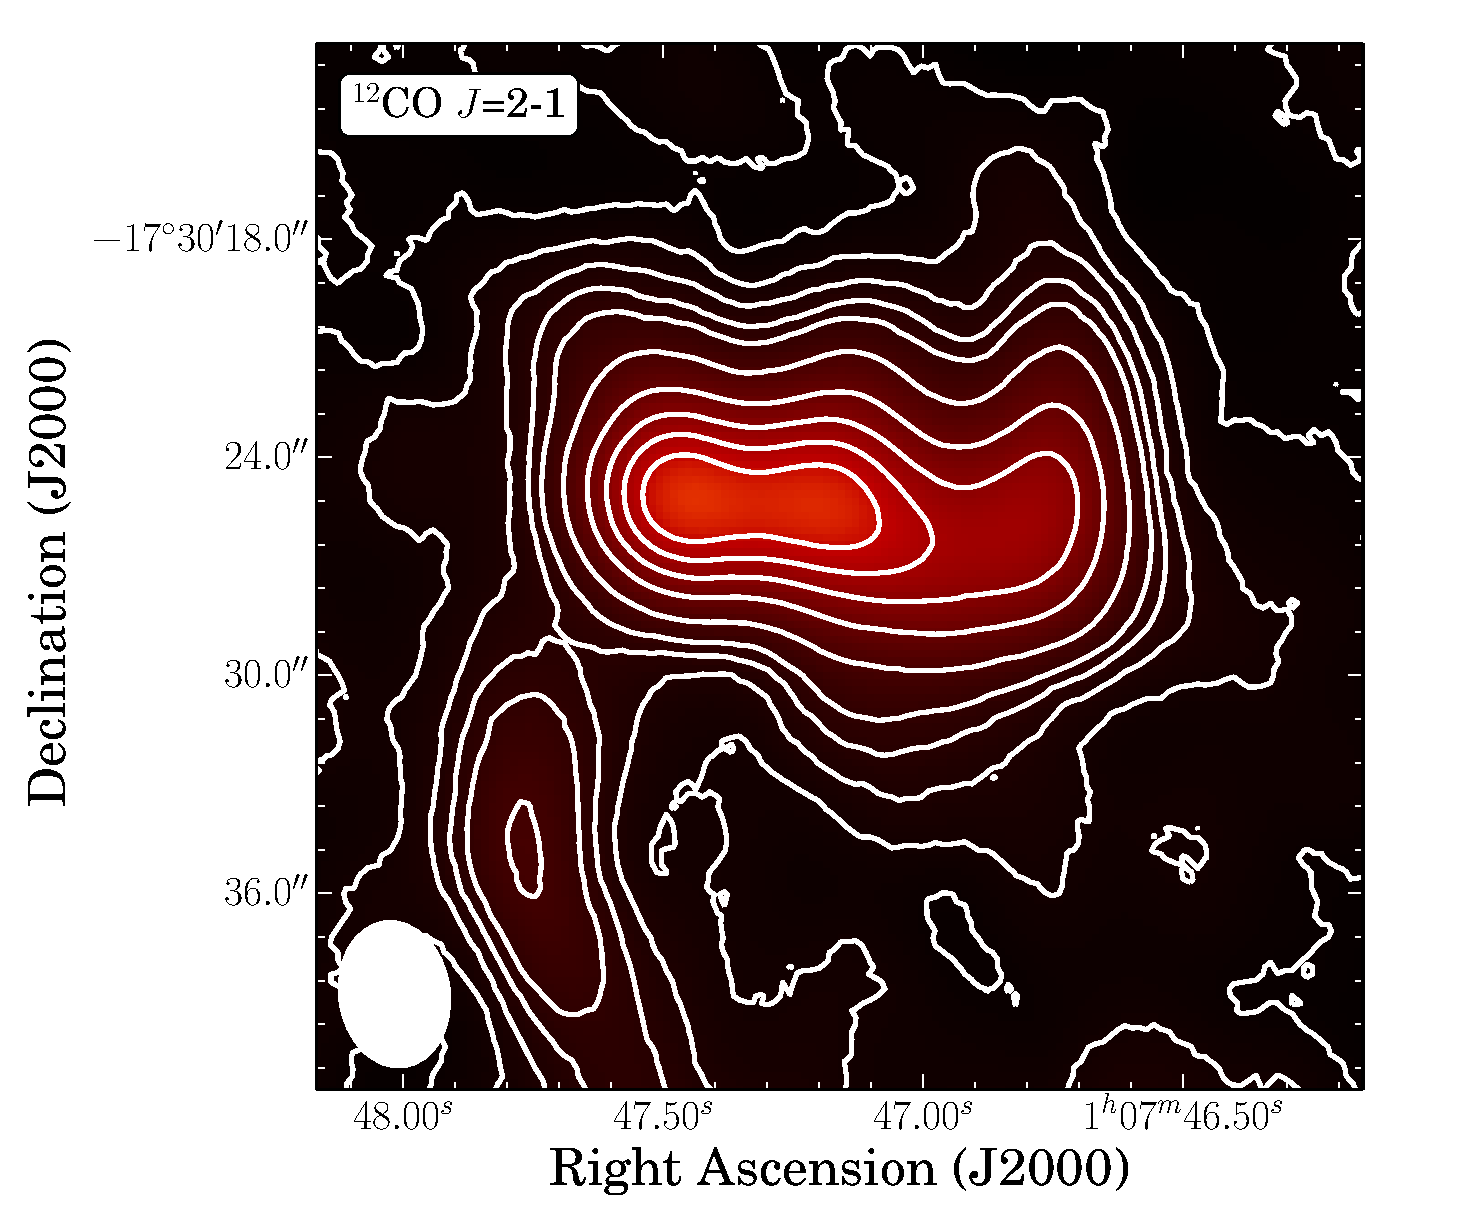
\includegraphics[ scale=0.3]{Chapter-2/Figures/fig1a.eps}  & 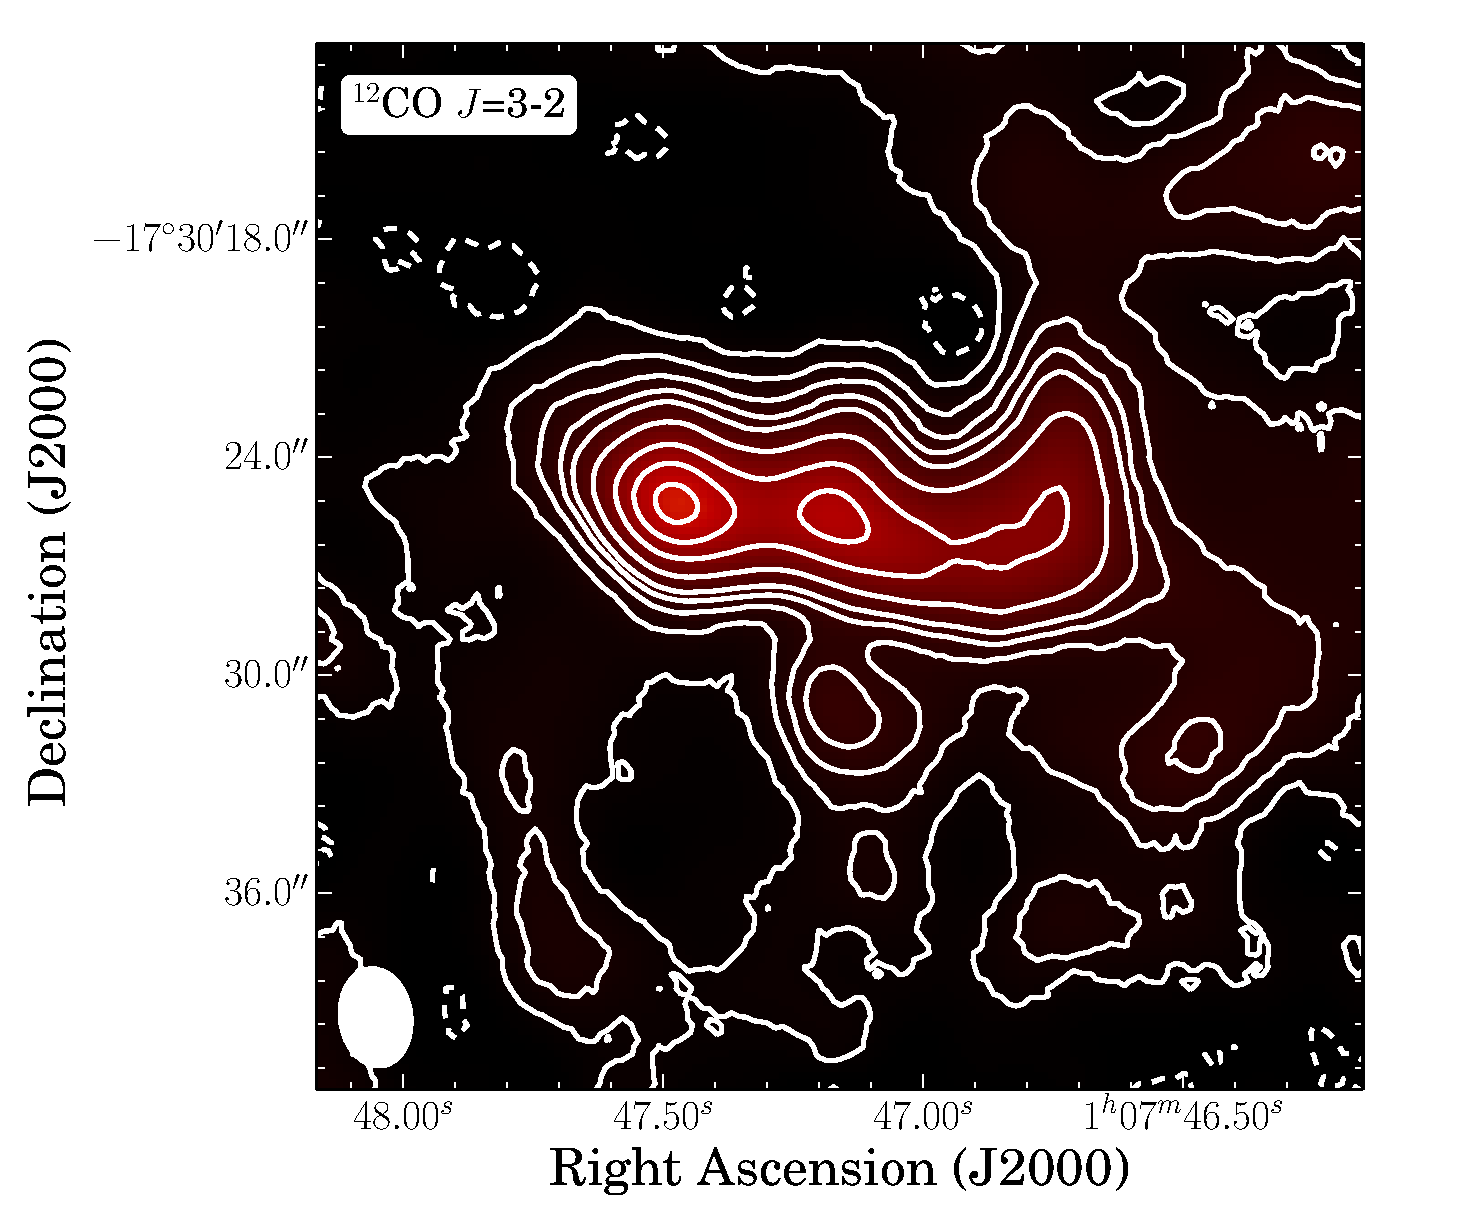
\includegraphics[scale=0.3]{Chapter-2/Figures/fig1b.eps} \\
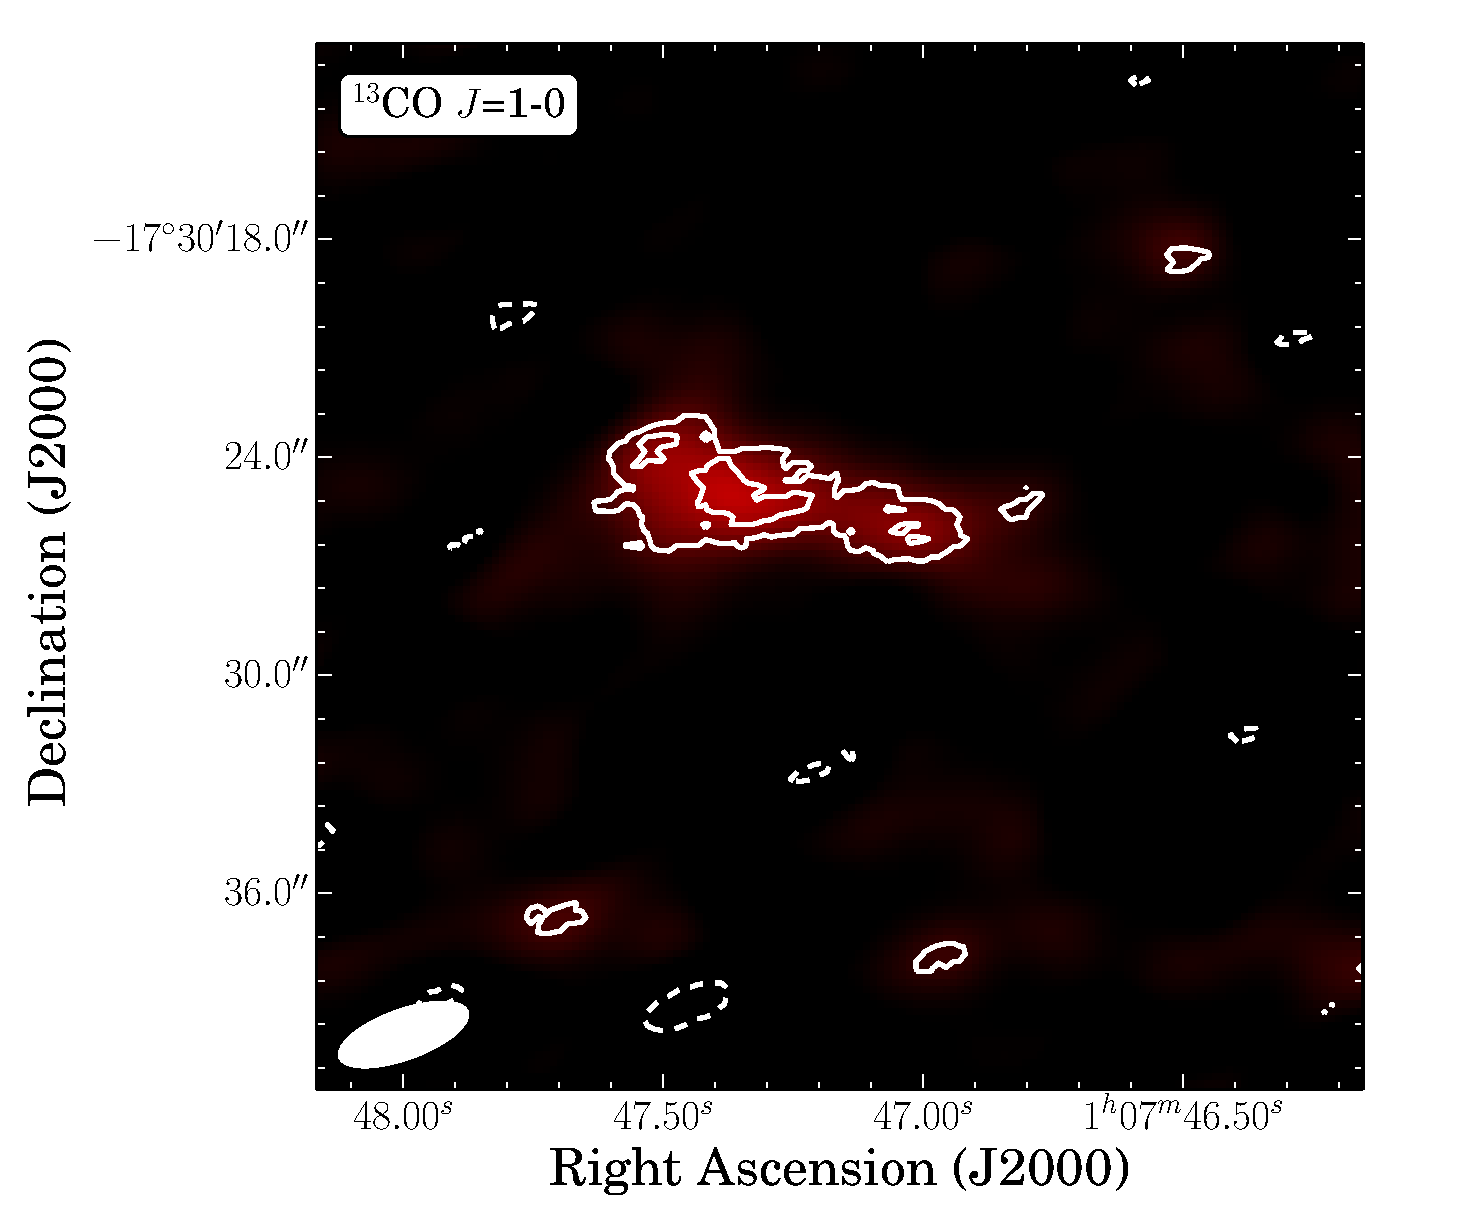
\includegraphics[scale=0.3]{Chapter-2/Figures/fig1c.eps} & 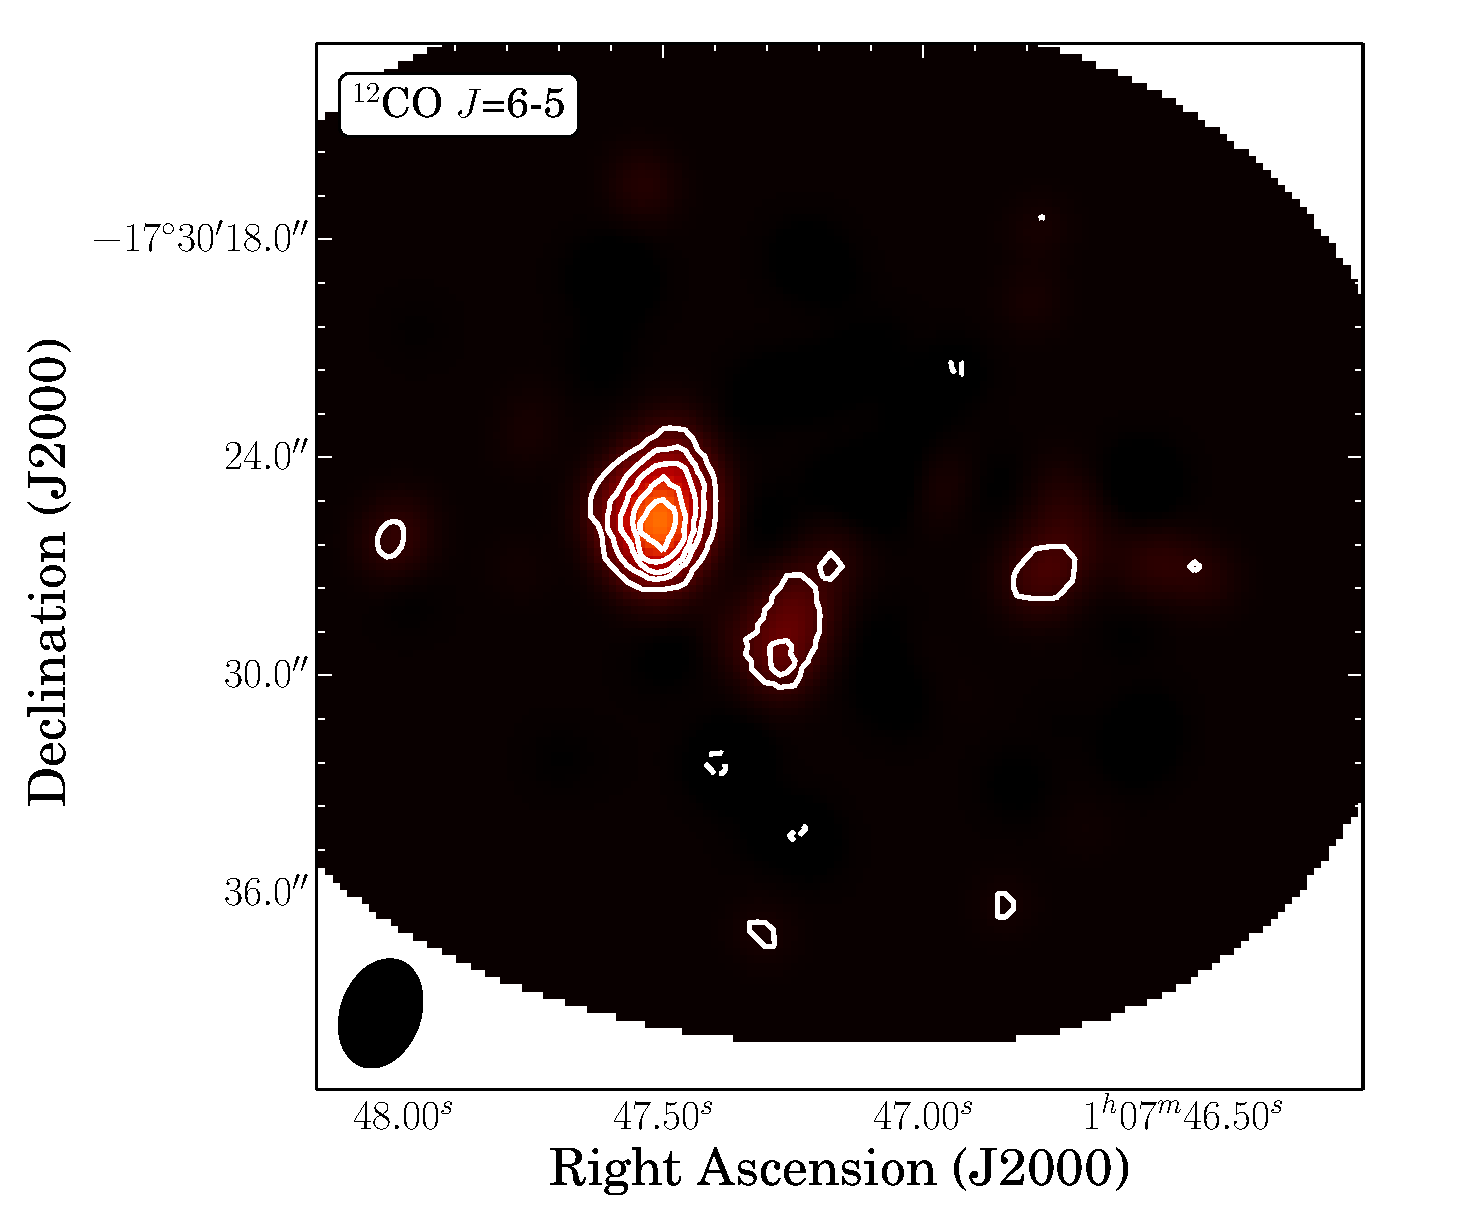
\includegraphics[scale=0.3]{Chapter-2/Figures/fig1d.eps} \\
\end{array}$
\caption[]{(\textit{Top Left }) $^{12}$CO J=2-1 map with the recovered short spacings from the JCMT. The contours correspond to -7.5, -4.5, -1.5, 1.5, 4.5, 7.5, 10.5, 13.5, 20, 30, 40, 50, 60 $\times$ 3.5 Jy beam$^{-1}$ km s$^{-1}$ (\textit{Top Right}) $^{12}$CO J=3-2 map with the recovered short spacings from the JCMT. The contours correspond to  -7.5, -4.5, -1.5, 1.5, 4.5, 7.5, 10.5, 13.5, 20, 30, 40, 50 $\times$ 7 Jy beam$^{-1}$ km s$^{-1}$. (\textit{Bottom Left}) \tcoone\ map with contours corresponding to -2, 2, 4, 6 $\times$ the 1$\sigma$ value of 0.25 Jy beam$^{-1}$ km s$^{-1}$. (\textit{Bottom Right}) \cosix\ map with contours corresponding to  --2, 2, 4, 6, 8, 10 $\times$ the 1$\sigma$ value of 16.4 Jy beam$^{-1}$ km s$^{-1}$. All maps have been corrected for the primary beam. Negative flux is denoted by dashed contours. }
\label{SMAmaps}
\end{figure}

\begin{figure}[h] %%%FIGURE 2
\centering
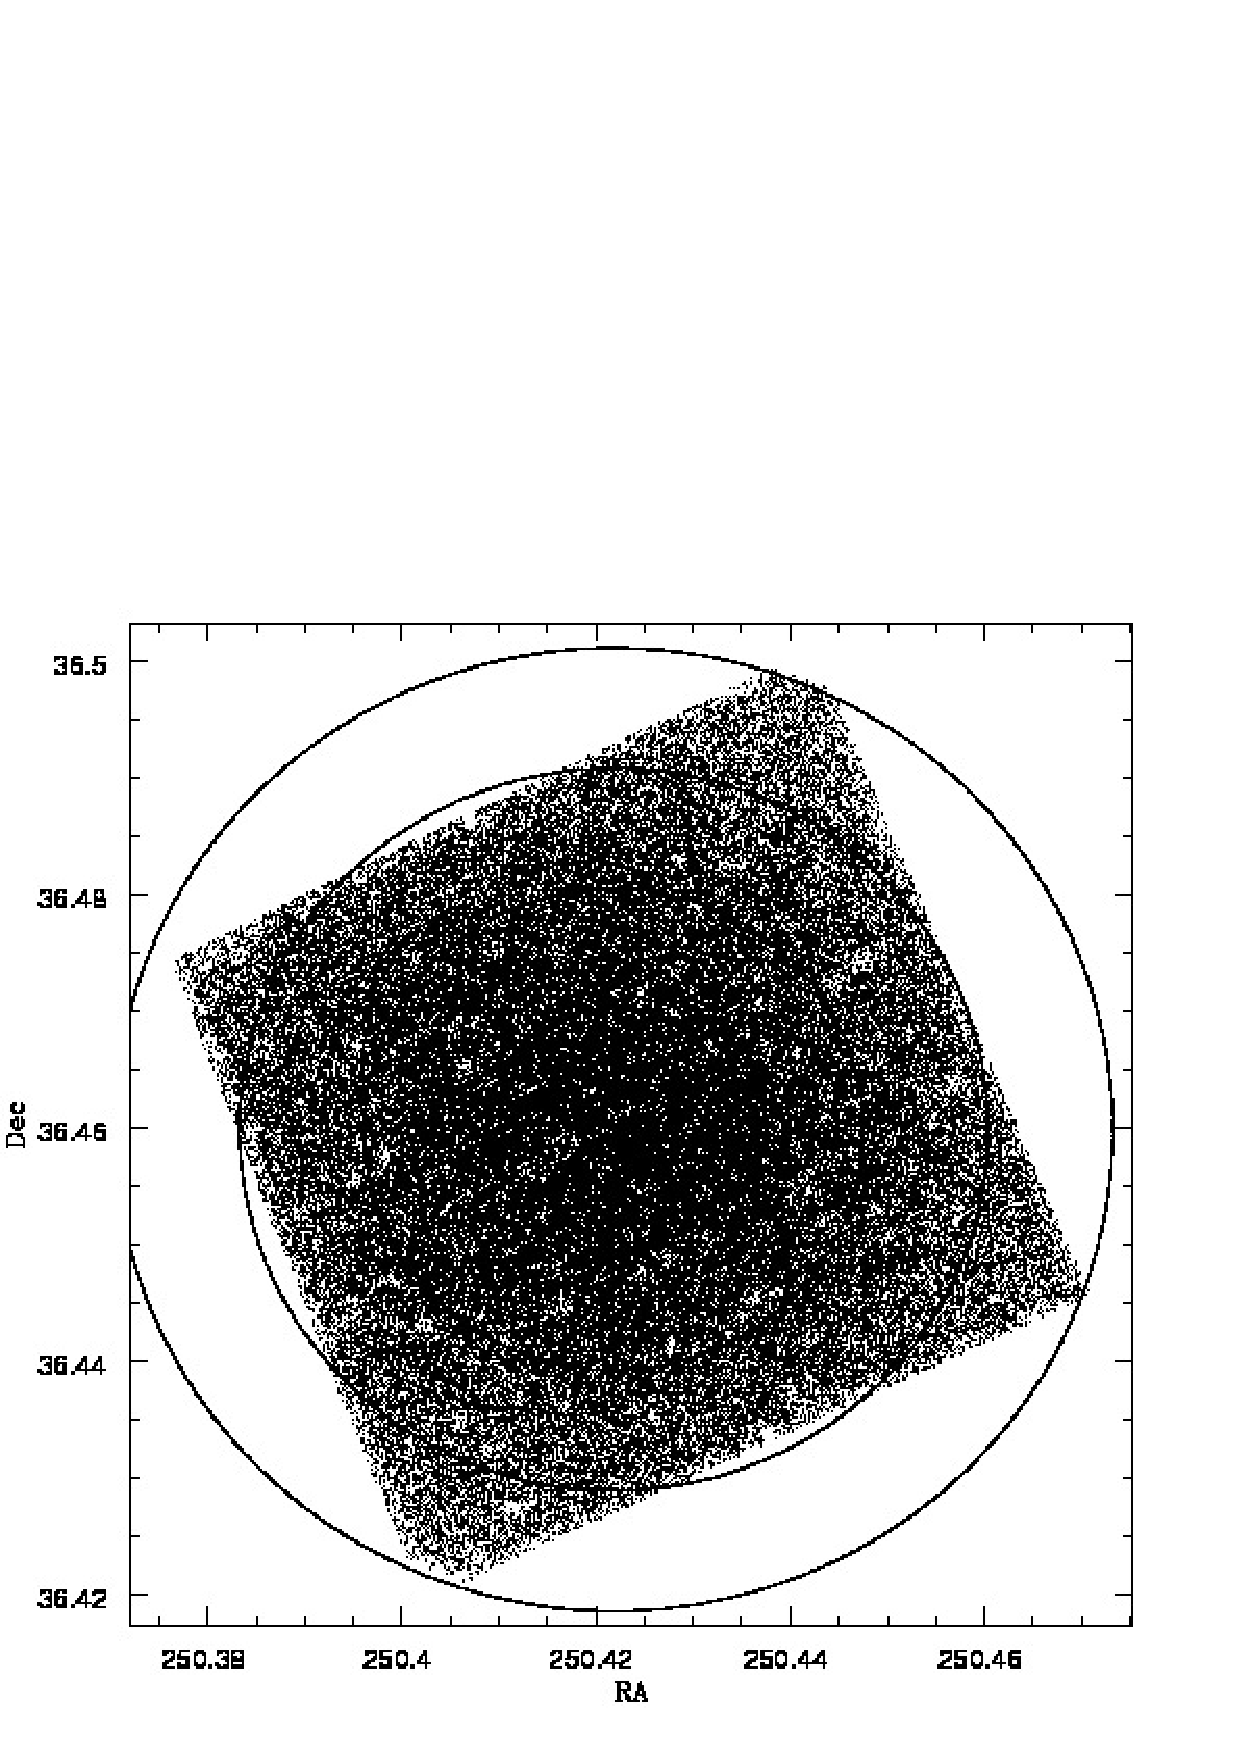
\includegraphics[scale=0.5,angle=-90]{Chapter-2/Figures/fig2.pdf} 
\caption[]{Peak spectrum of the \cosix\ emission for VV 114E.}
\label{Inte}
\end{figure}

\begin{figure}[h] %%%FIGURE 3a
\centering
$\begin{array}{c@{\hspace{0.5in}}c}
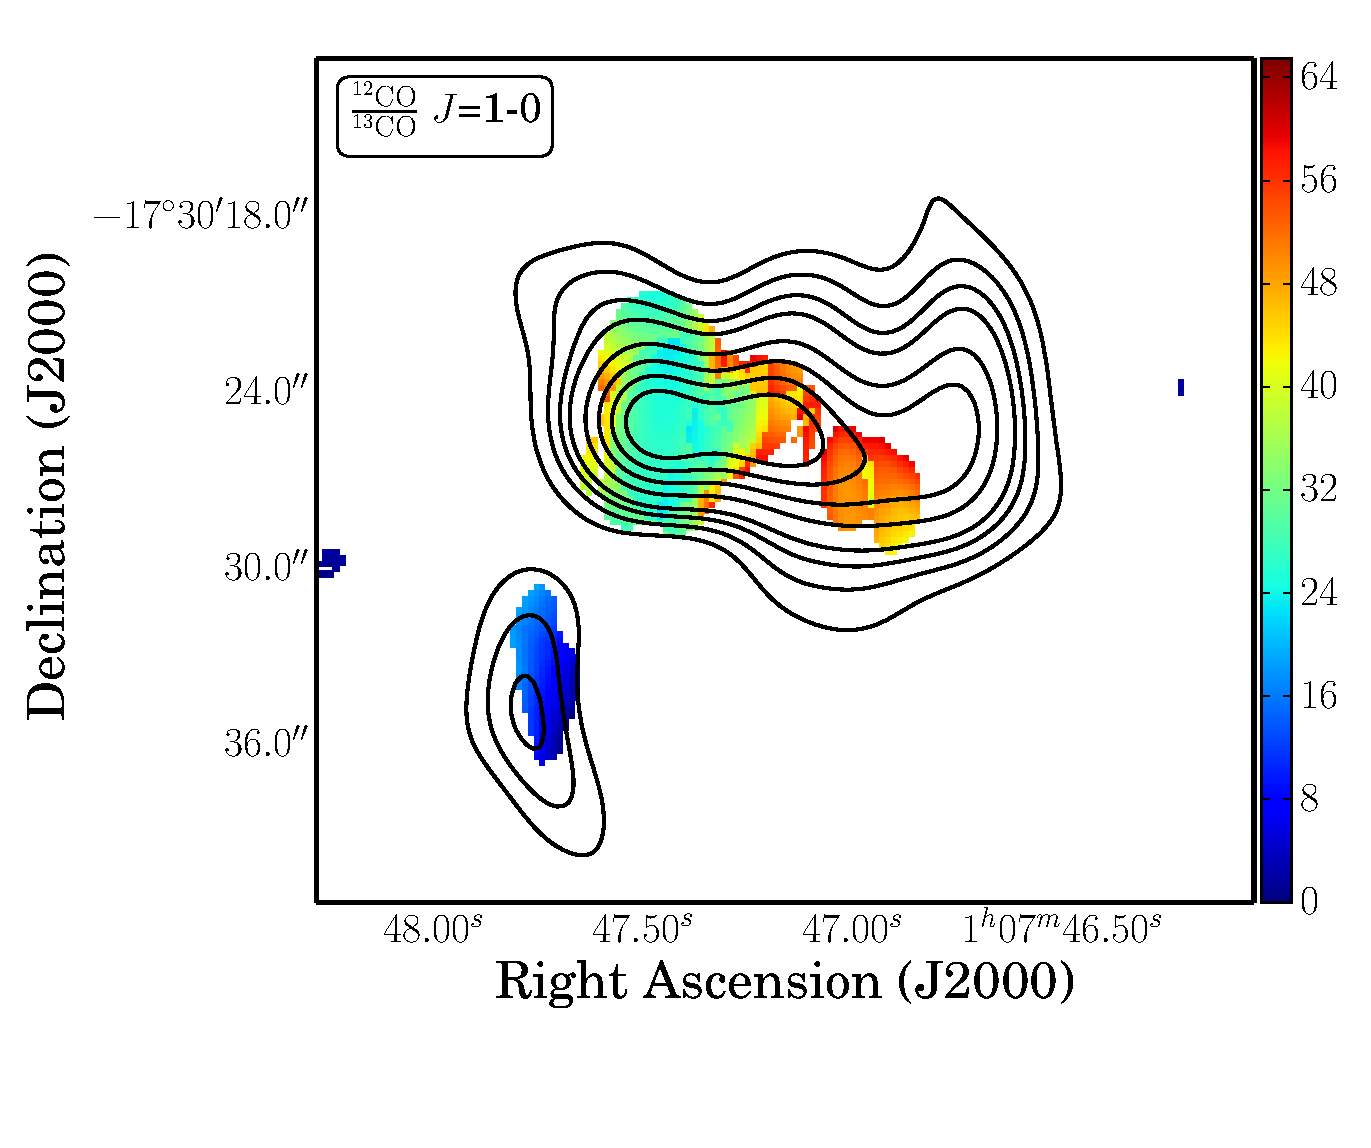
\includegraphics[scale=0.35]{Chapter-2/Figures/fig3f.eps} & 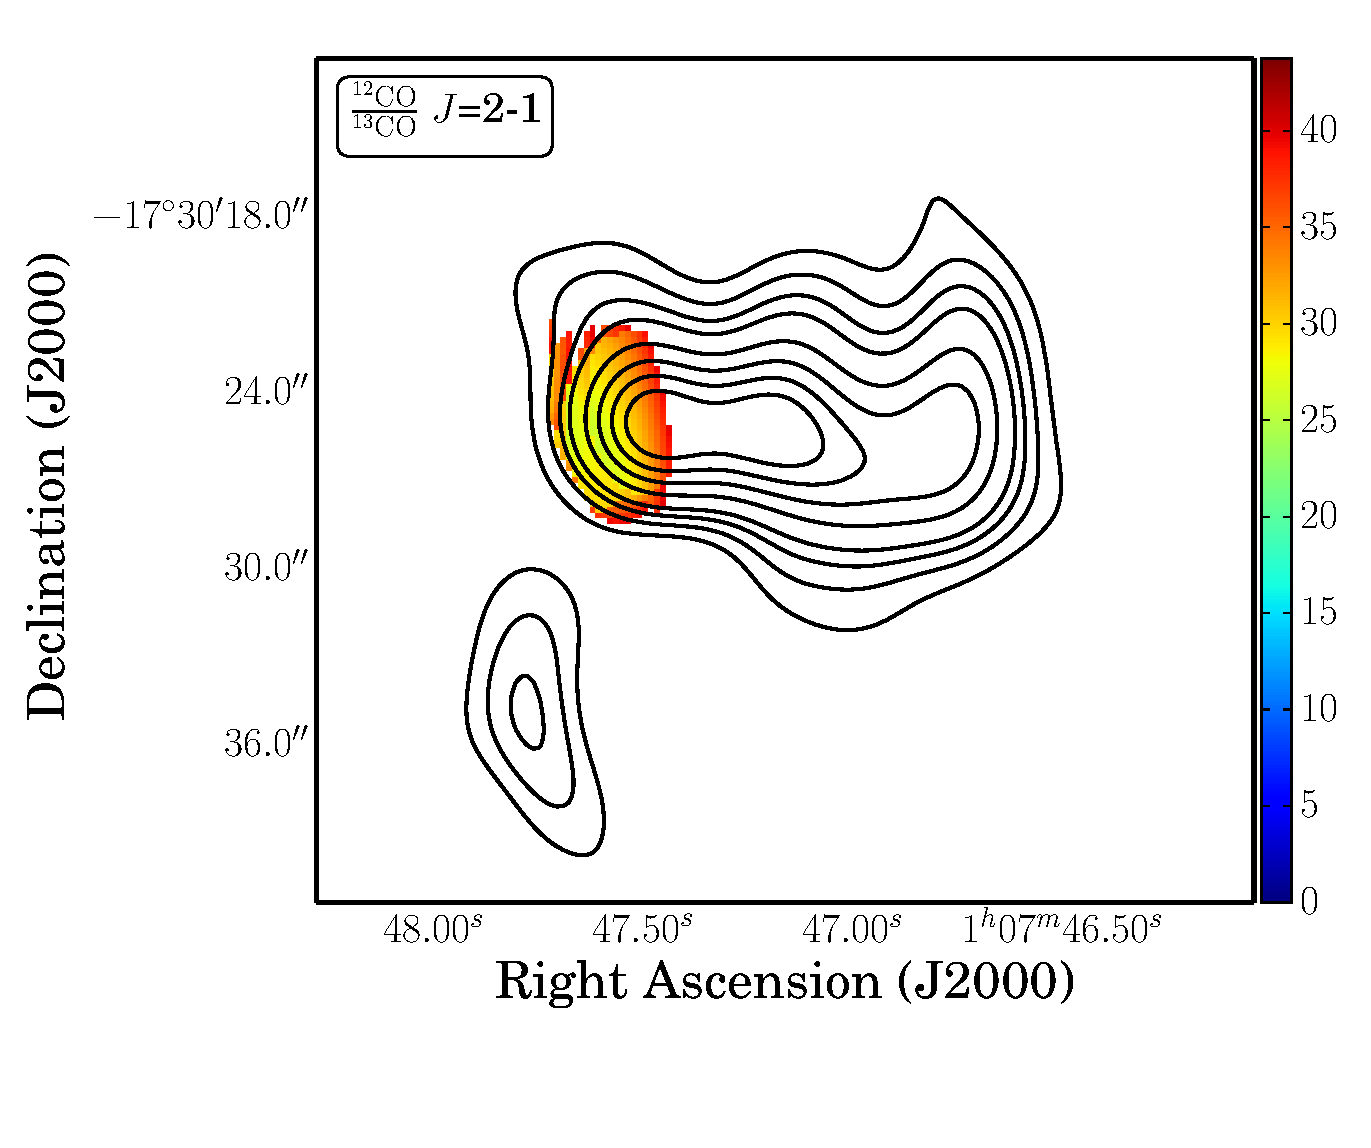
\includegraphics[scale=0.35]{Chapter-2/Figures/fig3a.eps} \\
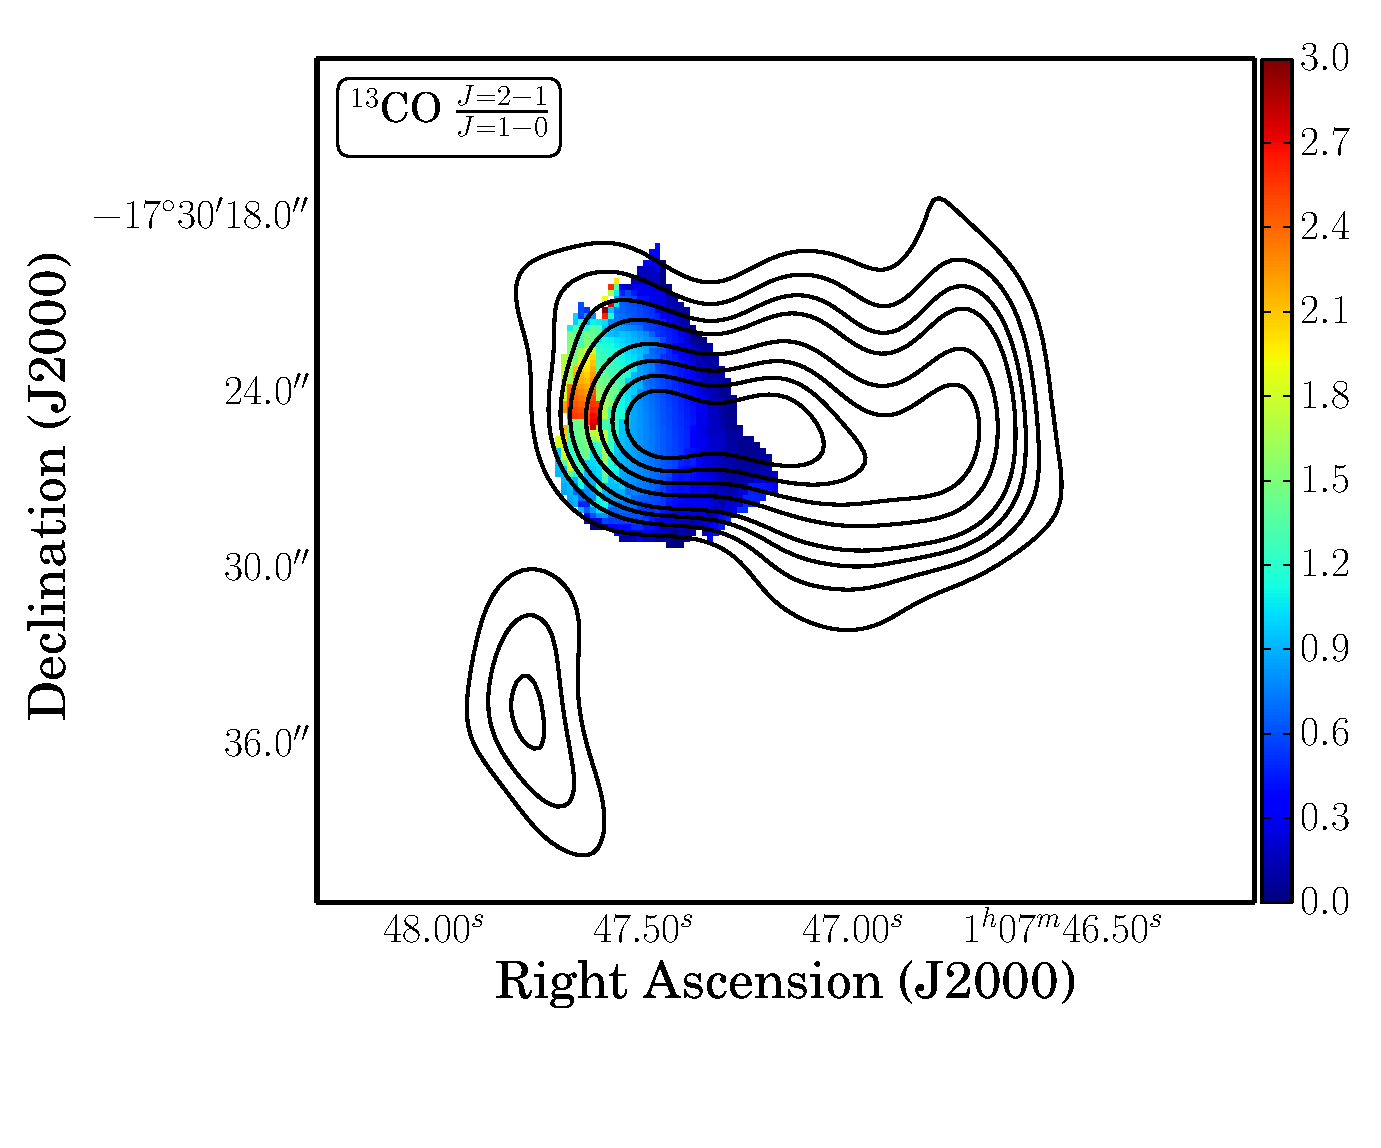
\includegraphics[scale=0.35]{Chapter-2/Figures/fig3g.eps} & 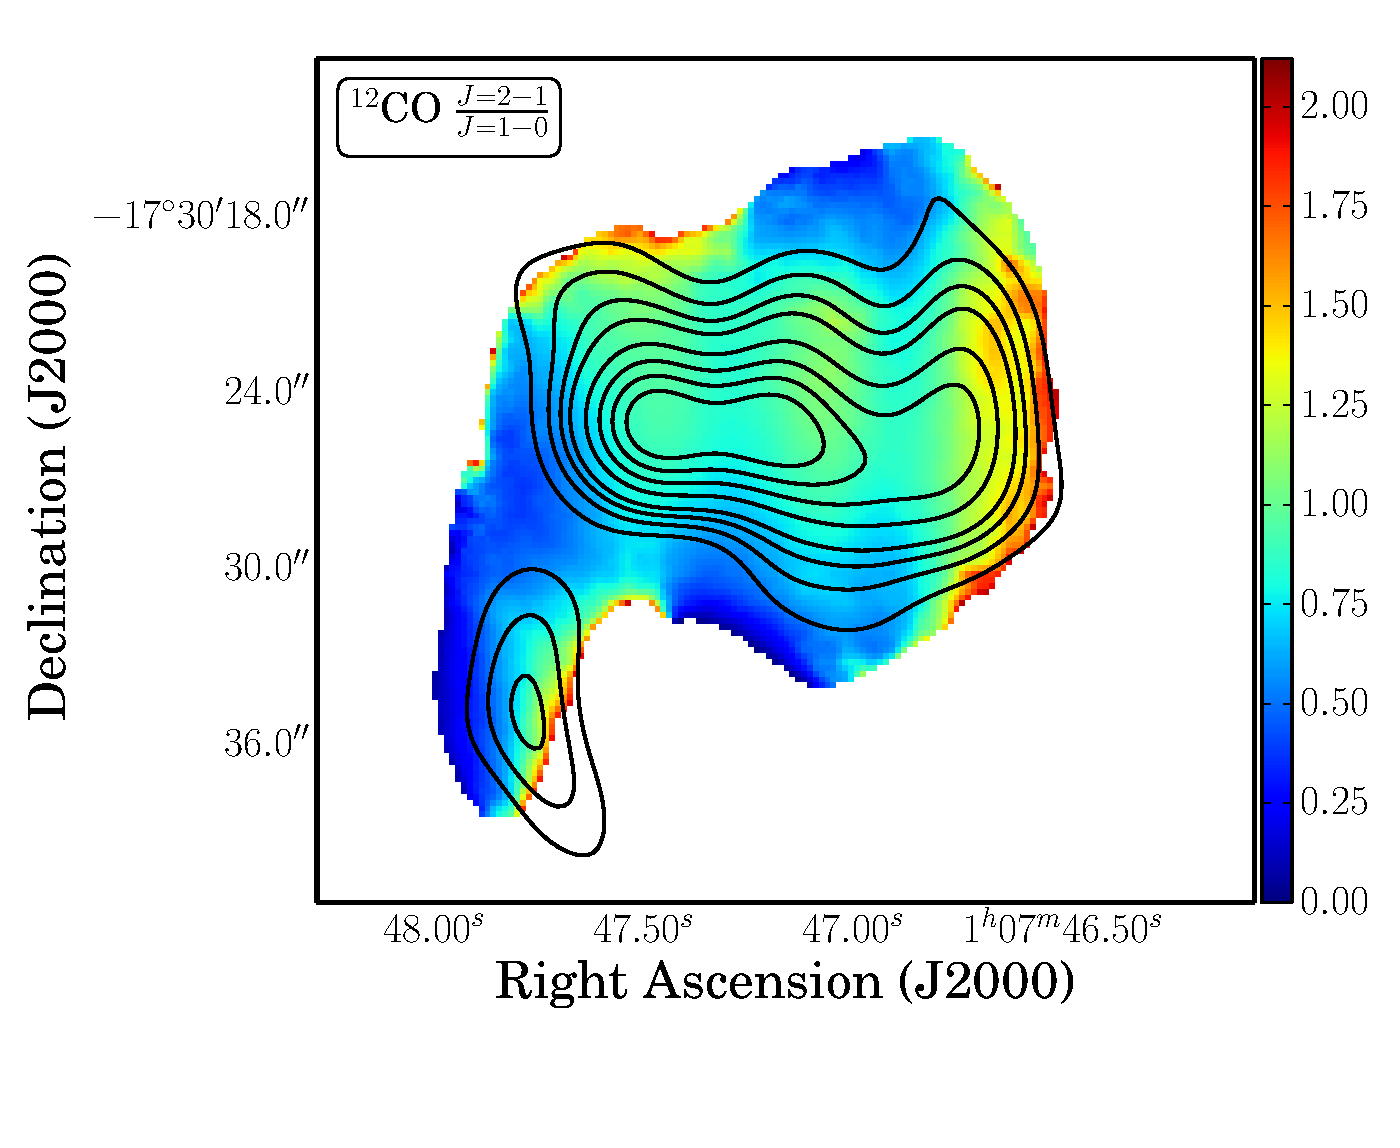
\includegraphics[scale=0.35]{Chapter-2/Figures/fig3b.eps} \\
\end{array}$
\caption[Line ratio maps]{Line ratio maps: (\textit{Top Left}) $^{13}$CO $\frac{J=2-1}{J=1-0}$ ; (\textit{Top Right}): $\frac{\mathrm{^{12}CO}}{\mathrm{^{13}CO}}$ $J$=2-1; (\textit{Bottom Left}) $\frac{\mathrm{^{12}CO}}{\mathrm{^{13}CO}}$ $J$=1-0; (\textit{Bottom Right}) $^{12}$CO $\frac{J=2-1}{J=1-0}$. Only emission that is $>$ 3$\sigma$ in both maps is included. Contours of \cotwo\ are shown to aid comparison between the maps. }
\label{RatioMaps}
\end{figure}

\begin{figure}[h] %%%FIGURE 4
\centering
$\begin{array}{c@{\hspace{0.5in}}c}

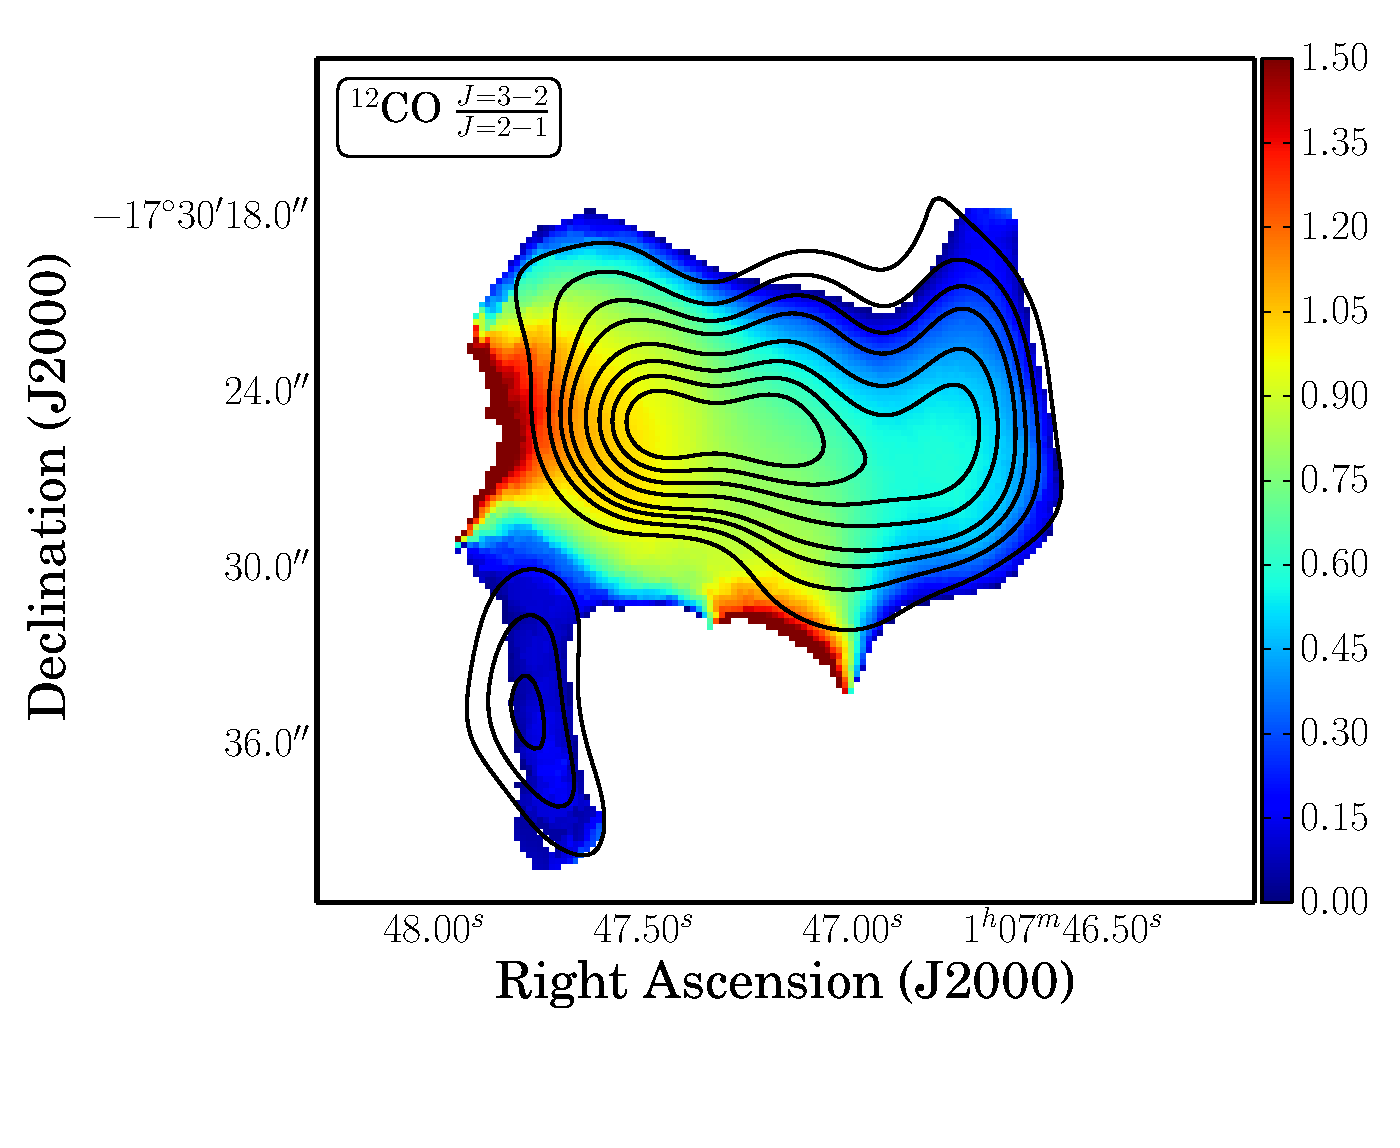
\includegraphics[scale=0.35]{Chapter-2/Figures/fig3c.eps} & 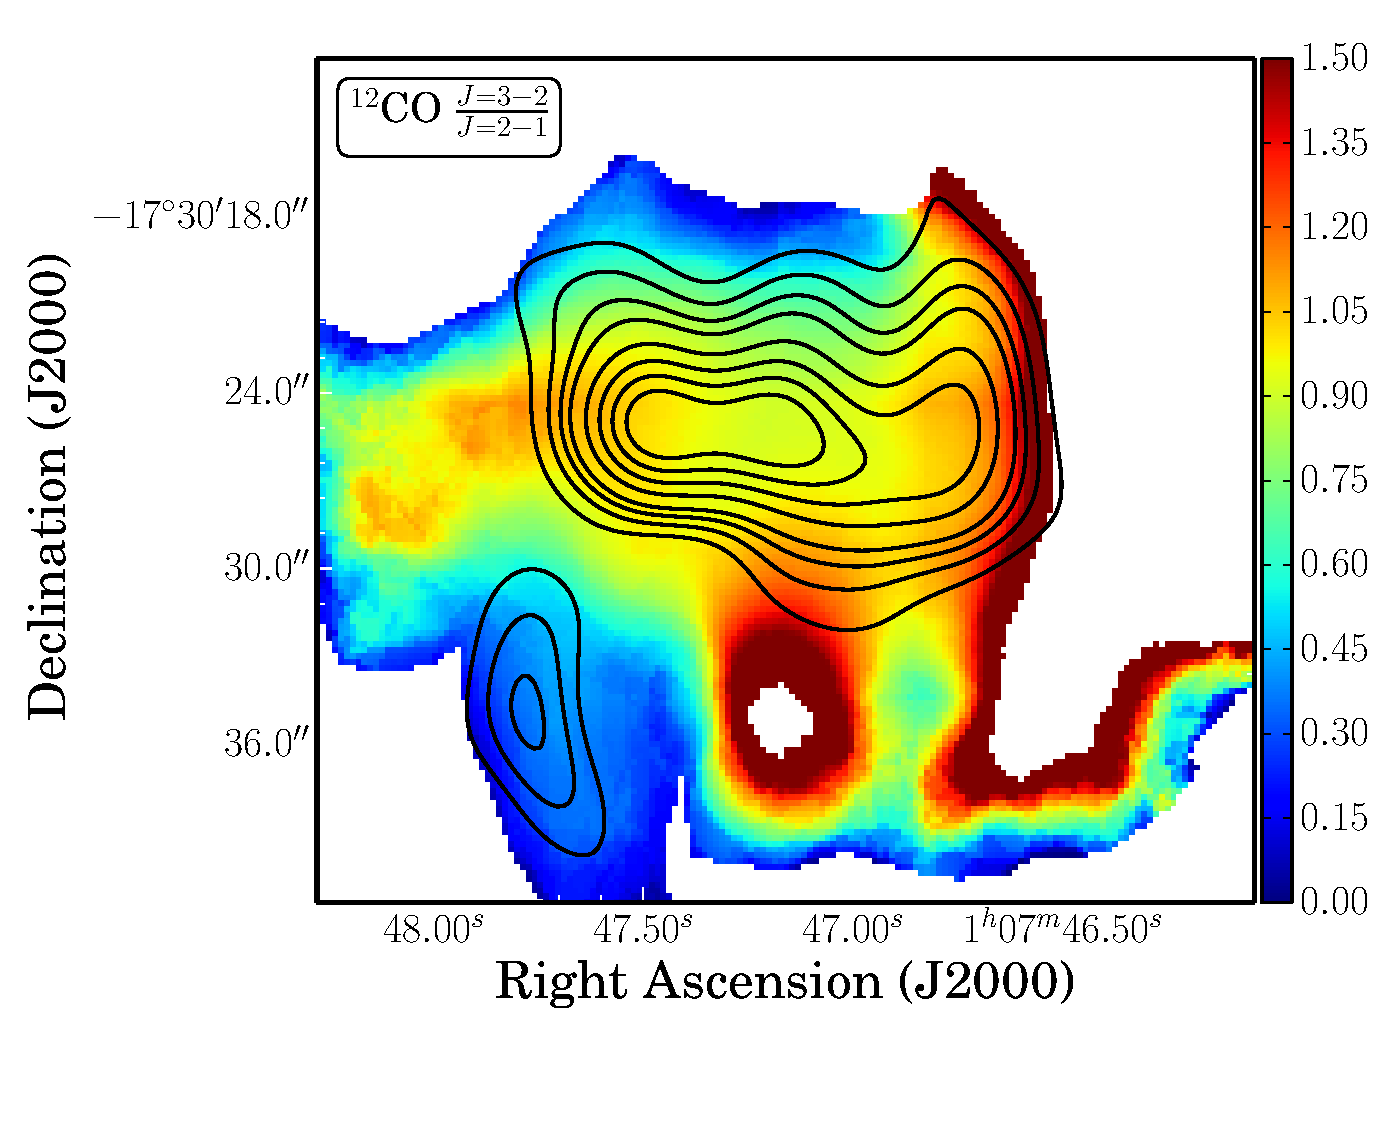
\includegraphics[scale=0.35]{Chapter-2/Figures/fig3d.eps} \\ 
 \end{array}$
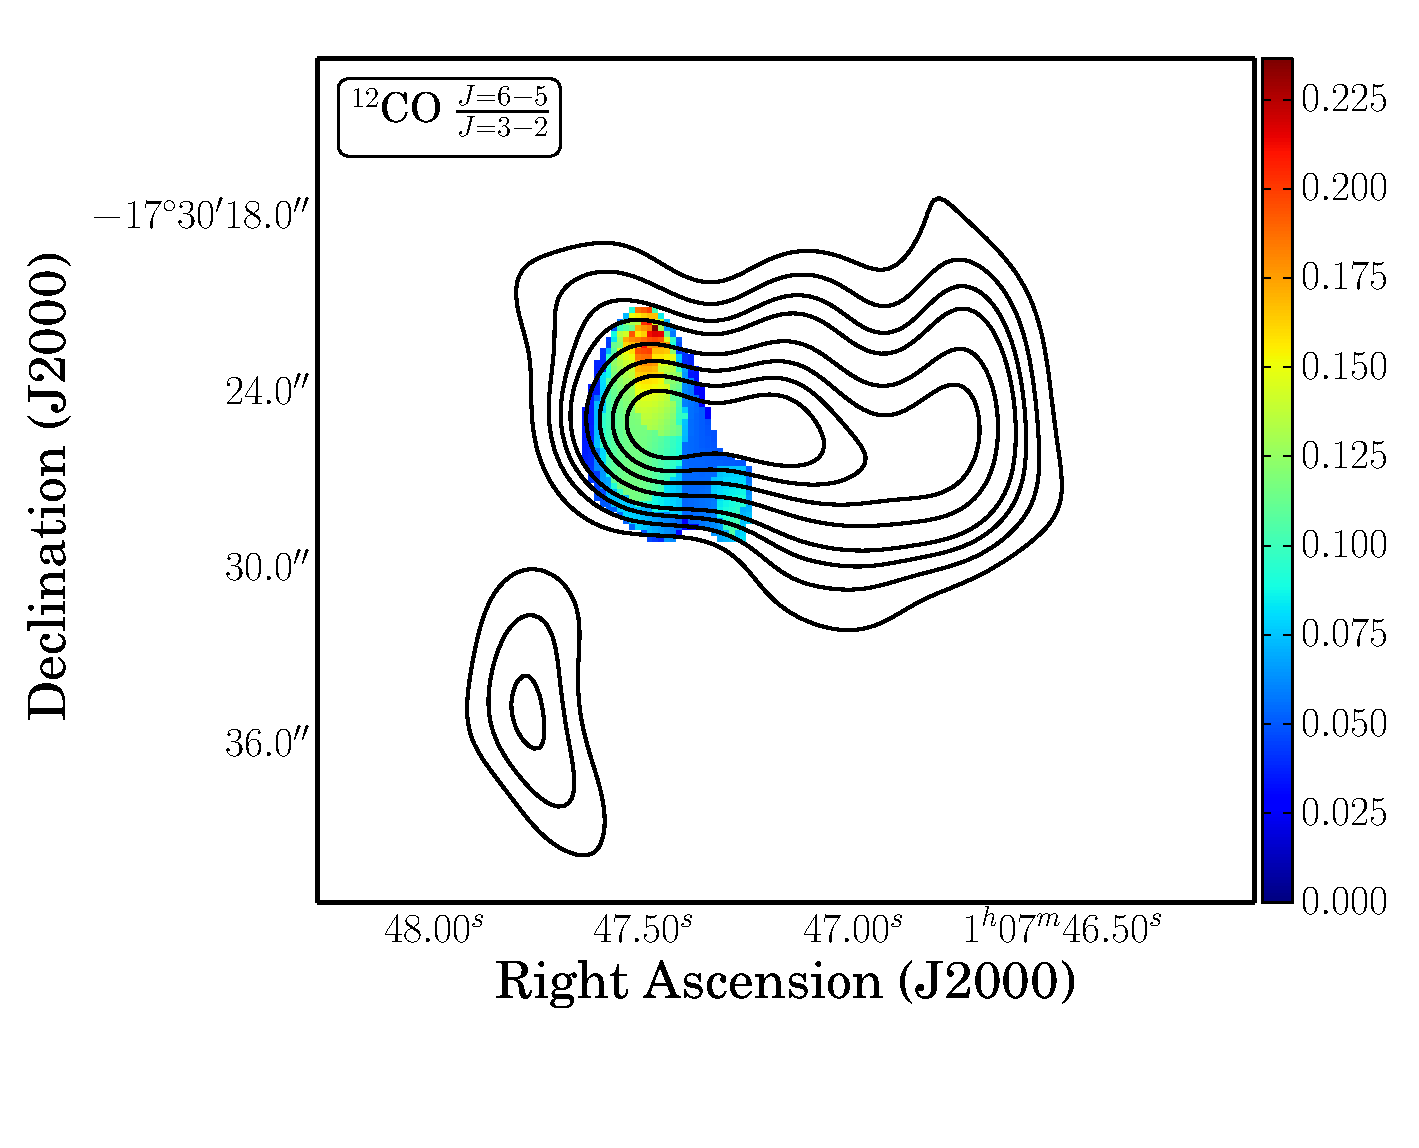
\includegraphics[scale=0.35]{Chapter-2/Figures/fig3e.eps} 
\caption[Line ratio maps]{Line ratio maps: (\textit{Top Left}) SMA only $^{12}$CO $\frac{J=3-2}{J=2-1}$; (\textit{Top Right}): SMA + JCMT  $^{12}$CO $\frac{J=3-2}{J=2-1}$; (\textit{Bottom}):  $^{12}$CO $\frac{J=6-5}{J=3-2}$. Contours and emission cutoffs as in Figure 3. }
\label{RatioMaps}
\end{figure}

\begin{figure}[h] %%%FIGURE 5
\centering
\includegraphics[scale=0.8]{Chapter-2/Figures/fig4_cosled.eps} 
\caption[]{$^{12}$CO (\textit{red circles}) and $^{13}$CO (\textit{blue diamonds}) SLEDs of VV 114E using Grid 2 solutions. The dashed lines are the fitted SLEDs from the radiative transfer analysis.}
\label{cosled}
\end{figure}

\begin{figure}[h] %%%FIGURE 6
\centering
$\begin{array}{cc}
\includegraphics[scale=0.45]{Chapter-2/Figures/fig5a_Tempdist.eps} & \includegraphics[scale=0.45]{Chapter-2/Figures/fig5b_Densdist.eps} \\ 
\end{array}$
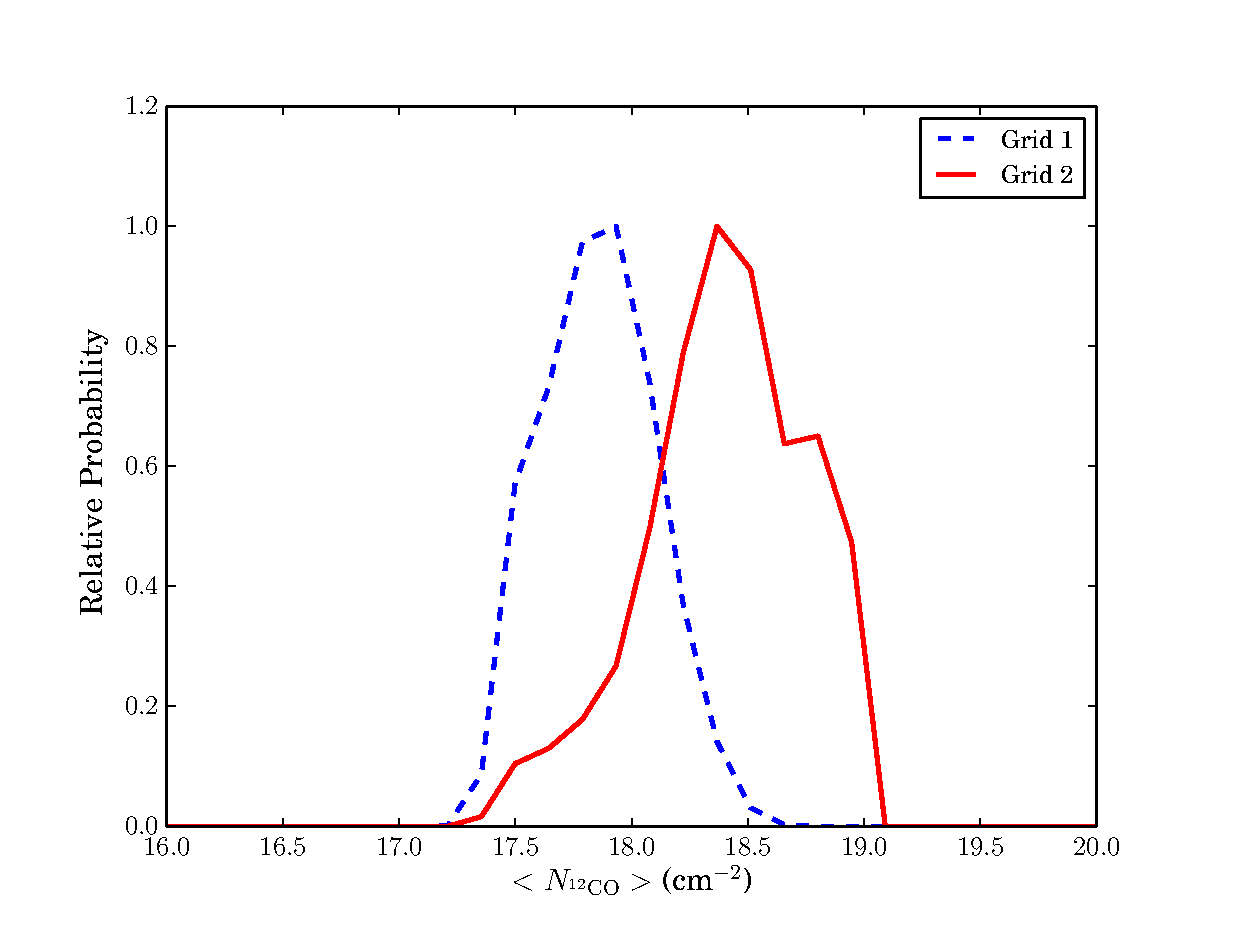
\includegraphics[scale=0.45]{Chapter-2/Figures/fig5c_BACDdist.eps}\\
\caption[distrib]{One-dimensional probability distributions for \tkin\ (top), \nhtwo\ (middle) and $<$\nco$>$ (bottom). Both Grid 1 and Grid 2 solutions are shown to display the difference in the solutions with differing \xco\ values. }
\label{}
\end{figure}

\begin{figure}[h] %%%FIGURE 7
\centering
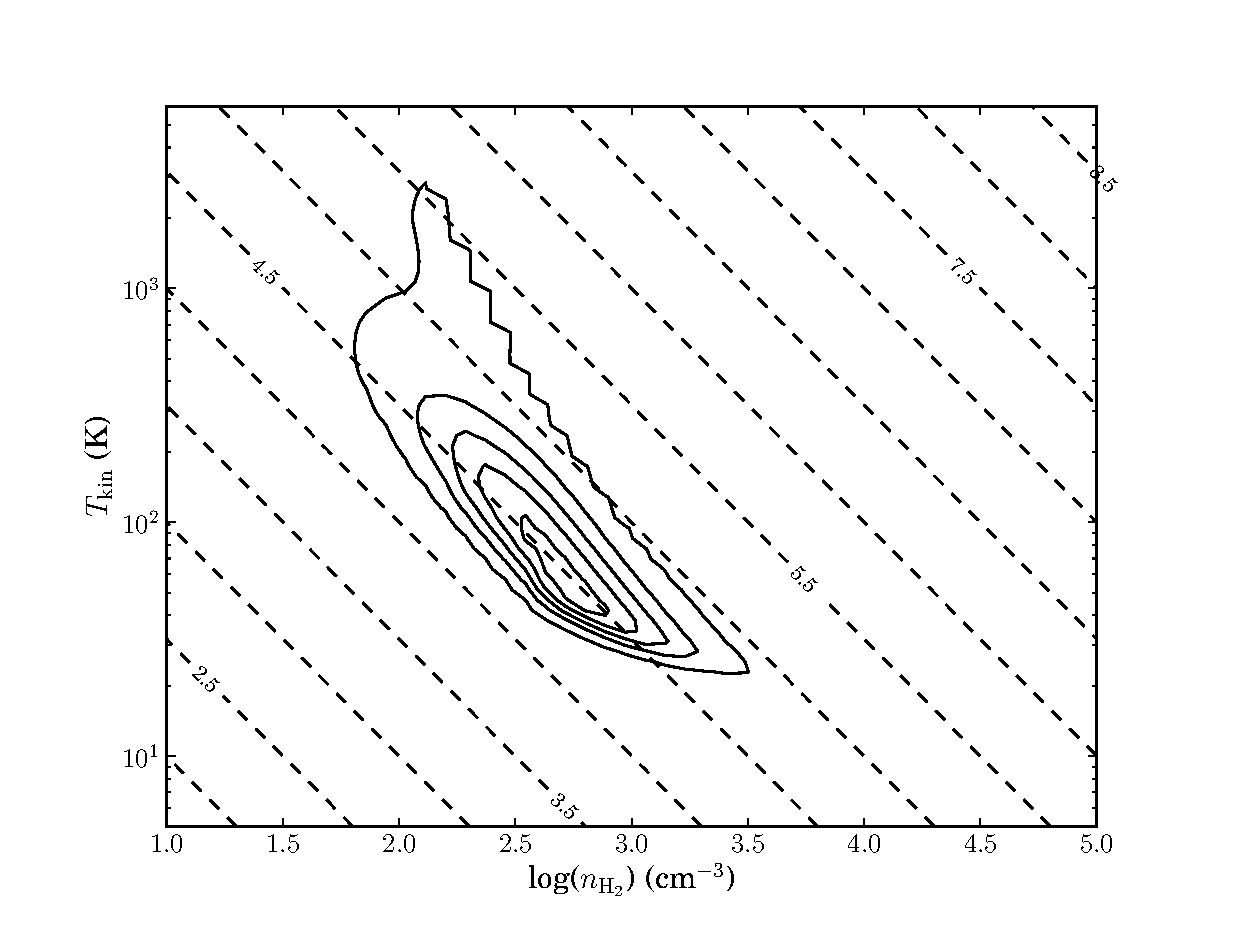
\includegraphics[scale=0.8]{Chapter-2/Figures/fig6_contour.eps} 
\caption[contours]{Two-dimensional distribution for \tkin\ vs. \nhtwo\ using Grid 2 solutions. Diagonal lines indicate pressure in log (K cm$^{-3}$). Contour levels are 10$\%$, 30$\%$, 50$\%$, 70$\%$ and 90$\%$ of the maximum likelihood.}
\label{}
\end{figure}

%%%%%%%%%%TABLES%%%%%%%%%%%%%%%


\begin{deluxetable}{cccccc} %TABLE 1
\tablecolumns{6}
\tablewidth{0pt}
\tablecaption{Data For VV 114}
\label{smasum}
\tablehead{\colhead{Transition Line} & \colhead{Interferometric Flux\tablenotemark{a}} & \colhead{JCMT Flux\tablenotemark{a}} &\colhead{JCMT + SMA Flux\tablenotemark{a}}& \colhead{Beam} & \colhead{rms}\\ \colhead{} & \colhead{(Jy km s$^{-1}$)}& \colhead{(Jy km s$^{-1}$)}& \colhead{(Jy km s$^{-1}$)} & \colhead{($\arcsec$)} & \colhead{(mJy/beam)\tablenotemark{b}} }
\startdata
\coone\tablenotemark{c}	&360 $\pm$ 20		&-&-&6.5 $\times$ 3.7 &25\\
\cotwo				&1280 $\pm$ 50	&2370 $\pm$ 60&2350 $\pm$ 70&4.0 $\times$ 3.0 &13\\
\cothree				&1890 $\pm$ 60	&4800 $\pm$ 200&4800 $\pm$ 60&2.8 $\times$ 2.0 &25\\
\cosix				&150 $\pm$ 40	&-&-&3.1 $\times$  2.2 &270\\
\tcoone\tablenotemark{d}&4.0 $\pm$ 0.3	&-&-&3.7 $\times$ 1.4 &2\\
\tcotwo				&12.0 $\pm$ 2.0	&-	&-&4.6 $\times$ 3.4 &10\\
\enddata
\tablenotetext{a}{measurement uncertainty only; calibration uncertainty is 20$\%$ (Paper I).  }
\tablenotetext{b}{rms values for a 20 km s$^{-1}$ channel width for all lines except \tcoone\ and \tcotwo\ which uses 40 km s$^{-1}$ and 50 km s$^{-1}$ channel widths, respectively.}
\tablenotetext{c}{OVRO map published in Yun et al. (1994)}
\tablenotetext{d}{ALMA Cycle 0 map}

\end{deluxetable}
\begin{deluxetable}{lccccccc} %%TABLE2
\tablecolumns{8}
\rotate
\tablewidth{0pt}
\tablecaption{CO Line Ratios of VV 114\tablenotemark{a}}
\label{line}
\tablehead{\colhead{Region} & \colhead{$^{12}$CO $\frac{J=6-5}{J=3-2}$} &  \colhead{$^{12}$CO $\frac{J=3-2}{J=2-1}$\tablenotemark{b}} &  \colhead{$^{12}$CO $\frac{J=3-2}{J=2-1}$\tablenotemark{c}} &\colhead{$^{12}$CO $\frac{J=2-1}{J=1-0}$} &\colhead{$^{13}$CO $\frac{J=2-1}{J=1-0}$} & \colhead{$\frac{\mathrm{^{12}CO}}{\mathrm{^{13}CO}}$ J=1-0} & \colhead{$\frac{\mathrm{^{12}CO}}{\mathrm{^{13}CO}}$ J=2-1} }
\startdata
VV 114E	&	0.13 $\pm$ 0.05	& 	0.99 $\pm$ 0.28	&0.95 $\pm$ 0.27 & 0.93 $\pm$ 0.26 & 0.63 $\pm$ 0.18 & 25.6 $\pm$ 7.2& 37.7 $\pm$ 5.3\\
VV 114C&	$<$ 0.03\tablenotemark{d} &0.92$\pm$0.26 &0.74$\pm$0.21 &0.89$\pm$0.25 & -- &  $>$ 57\tablenotemark{e} &$>$	77\tablenotemark{e}	\\
VV 114W	&	$<$ 0.04\tablenotemark{d} &1.01$\pm$0.28 &0.57$\pm$0.16 &0.91$\pm$0.26 & --& $>$ 42\tablenotemark{e} &$>$ 60\tablenotemark{e}	\\
\enddata
\tablenotetext{a}{All ratios are in terms of integrated brightness temperatures at the peak position of \cothree. Uncertainties include calibration and measurement uncertainties. All maps were degraded to a resolution of 6.5$\arcsec$ $\times$ 3.7$\arcsec$.}
\tablenotetext{b}{Using short spacing corrected maps.}
\tablenotetext{c}{Using SMA only maps.}
\tablenotetext{d}{Ratios are upper limits using the 3$\sigma$ noise level for \cosix.}
\tablenotetext{e}{Ratios are lower limits using 3$\sigma$ noise level for \tcoone\ and \tcotwo.}
\end{deluxetable}


\begin{deluxetable}{ccccc} %%%TABLE 3
\tablecolumns{5}
\tablewidth{0pt}
\tablecaption{Source Size and Dynamical Mass}
\label{linewidth}
\tablehead{\colhead{Region} & \colhead{Velocity FWHM\tablenotemark{a}}&  \multicolumn{2}{c}{Deconvolved Source Diameter\tablenotemark{b}} & \colhead{$M_{\rm{dyn}}$} \\ \colhead{} & \colhead{(km s$^{-1}$)}&  \colhead{(arcsec)} & \colhead{(kpc)} & \colhead{(10$^{9}$ $M_{\odot}$)} }
\startdata
VV 114E	&	150	&	(4.1 $\pm$ 0.1) x (1.8 $\pm$ 0.2)	&	(1.71 $\pm$ 0.04) x (0.75 $\pm$ 0.08)	& 	2.4 $\pm$ 0.3\\
VV 114W	&	200	&	(4.4 $\pm$ 0.3) x (2.3 $\pm$ 0.4)	&	(1.8 $\pm$ 0.1) x (1.0 $\pm$ 0.2)	&	5.3 $\pm$ 0.4 \\
VV 114C&	155/95\tablenotemark{c}	&	(7.3 $\pm$ 0.2) x (1.8 $\pm$ 0.3)	&	(3.04 $\pm$ 0.08) x (0.8 $\pm$ 0.1)	&	--\\
\enddata
\tablenotetext{a}{Uncertainty in velocity FWHM is 10 km s$^{-1}$}
\tablenotetext{b}{Beam size is 2.8$\arcsec$ $\times$ 2.0$\arcsec$}
%\tablenotetext{c}{Region A2 cannot be fit with a Gaussian because it is too close to region A}
\tablenotetext{c}{The central region spectrum is fitted with two Gaussian peaks.}
\end{deluxetable}


\begin{deluxetable}{ccccc} %%%%Table 4
\tablecolumns{4}
\tablewidth{0pt}
\tablecaption{Modeling Results\tablenotemark{a}}
\label{results}
\tablehead{ \colhead{} & \colhead{1DMax} & \colhead{4DMax} & \colhead{1$\sigma$ range}  }
\startdata
\tkin\ (K) &	51&		38&		42 -- 459  \\
\nhtwo\ (cm$^{-3}$) &	10$^{2.63}$ &		10$^{2.89}$&		10$^{2.07}$ -- 10$^{2.88}$  \\
\nco\ (cm$^{-2}$) &		10$^{19.58}$ &	10$^{20.03}$& 	10$^{18.87}$ -- 10$^{19.80}$   \\
\ff\ & 				10$^{-1.14}$ &	10$^{-1.14}$ &	10$^{-1.26}$ -- 10$^{-0.87}$   \\
$P$ (K cm$^{-3}$) &	10$^{4.58}$  &		10$^{4.58}$  & 	10$^{4.33}$ -- 10$^{4.88}$   \\
$<$\nco$>$ (cm$^{-2}$) & 10$^{18.37}$ & 	10$^{18.37}$ &	10$^{17.98}$ -- 10$^{18.71}$   \\
Mass (\msol) &			10$^{8.79}$& 	10$^{8.79}$&		10$^{8.40}$ -- 10$^{9.13}$ &   \\
\hline
\hline
\xco & 229 & 229 & 112 -- 603 \\
\nthreeco (cm$^{-2}$) & 10$^{17.13}$ & 10$^{17.13}$ & 10$^{16.75}$ -- 10$^{17.18}$ \\
\enddata
\tablenotetext{a}{ These are the modeling results for Grid 2.}

\end{deluxetable}


\begin{thebibliography}{37}
\expandafter\ifx\csname natexlab\endcsname\relax\def\natexlab#1{#1}\fi

\bibitem[{{Aalto} {et~al.}(1995){Aalto}, {Booth}, {Black}, \&
  {Johansson}}]{1995A&A...300..369A}
{Aalto}, S., {Booth}, R.~S., {Black}, J.~H., \& {Johansson}, L.~E.~B. 1995,
  \aap, 300, 369

\bibitem[{{Casoli} {et~al.}(1992){Casoli}, {Dupraz}, \&
  {Combes}}]{1992A&A...264...55C}
{Casoli}, F., {Dupraz}, C., \& {Combes}, F. 1992, \aap, 264, 55

\bibitem[{{Currie} {et~al.}(2008)}]{2008ASPC..394..650C}
{Currie}, M.~J. {et~al.} 2008, in Astronomical Society of the Pacific
  Conference Series, Vol. 394, Astronomical Data Analysis Software and Systems
  XVII, ed. R.~W. {Argyle}, P.~S. {Bunclark}, \& J.~R. {Lewis}, 650

\bibitem[{{Downes} \& {Solomon}(1998)}]{1998ApJ...507..615D}
{Downes}, D. \& {Solomon}, P.~M. 1998, \apj, 507, 615

\bibitem[{{Frayer} {et~al.}(1999){Frayer}, {Ivison}, {Smail}, {Yun}, \&
  {Armus}}]{1999AJ....118..139F}
{Frayer}, D.~T., {Ivison}, R.~J., {Smail}, I., {Yun}, M.~S., \& {Armus}, L.
  1999, \aj, 118, 139

\bibitem[{{Goldsmith} \& {Langer}(1978)}]{1978ApJ...222..881G}
{Goldsmith}, P.~F. \& {Langer}, W.~D. 1978, \apj, 222, 881

\bibitem[{{Greve} {et~al.}(2009){Greve}, {Papadopoulos}, {Gao}, \&
  {Radford}}]{2009ApJ...692.1432G}
{Greve}, T.~R., {Papadopoulos}, P.~P., {Gao}, Y., \& {Radford}, S.~J.~E. 2009,
  \apj, 692, 1432

\bibitem[{{Harris} {et~al.}(1991)}]{1991ApJ...382L..75H}
{Harris}, A.~I. {et~al.} 1991, \apjl, 382, L75

\bibitem[{{Henkel} {et~al.}(2010){Henkel}, {Downes}, {Wei{\ss}}, {Riechers}, \&
  {Walter}}]{2010A&A...516A.111H}
{Henkel}, C., {Downes}, D., {Wei{\ss}}, A., {Riechers}, D., \& {Walter}, F.
  2010, \aap, 516, A111

\bibitem[{{Ho} {et~al.}(2004){Ho}, {Moran}, \& {Lo}}]{2004ApJ...616L...1H}
{Ho}, P.~T.~P., {Moran}, J.~M., \& {Lo}, K.~Y. 2004, \apjl, 616, L1

\bibitem[{{Iono} {et~al.}(2004)}]{2004ApJ...616L..63I}
{Iono}, D. {et~al.} 2004, \apjl, 616, L63

\bibitem[{{Iono} {et~al.}(2009)}]{2009ApJ...695.1537I}
---. 2009, \apj, 695, 1537

\bibitem[{{Iono} {et~al.}(2013)}]{2013PASJ...65L...7I}
---. 2013, \pasj, 65, L7

\bibitem[{{Kamenetzky} {et~al.}(2011)}]{2011ApJ...731...83K}
{Kamenetzky}, J. {et~al.} 2011, \apj, 731, 83

\bibitem[{{Kamenetzky} {et~al.}(2012)}]{2012ApJ...753...70K}
---. 2012, \apj, 753, 70

\bibitem[{{Knop} {et~al.}(1994)}]{1994AJ....107..920K}
{Knop}, R.~A. {et~al.} 1994, \aj, 107, 920

\bibitem[{{Langer} \& {Penzias}(1990)}]{1990ApJ...357..477L}
{Langer}, W.~D. \& {Penzias}, A.~A. 1990, \apj, 357, 477

\bibitem[{{Le Floc'h} {et~al.}(2002)}]{2002A&A...391..417L}
{Le Floc'h}, E. {et~al.} 2002, \aap, 391, 417

\bibitem[{{Maloney} {et~al.}(1996){Maloney}, {Hollenbach}, \&
  {Tielens}}]{1996ApJ...466..561M}
{Maloney}, P.~R., {Hollenbach}, D.~J., \& {Tielens}, A.~G.~G.~M. 1996, \apj,
  466, 561

\bibitem[{{Mart{\'{\i}}n} {et~al.}(2010){Mart{\'{\i}}n}, {Aladro},
  {Mart{\'{\i}}n-Pintado}, \& {Mauersberger}}]{2010A&A...522A..62M}
{Mart{\'{\i}}n}, S., {Aladro}, R., {Mart{\'{\i}}n-Pintado}, J., \&
  {Mauersberger}, R. 2010, \aap, 522, A62

\bibitem[{{Matsushita} {et~al.}(2009)}]{2009ApJ...693...56M}
{Matsushita}, S. {et~al.} 2009, \apj, 693, 56

\bibitem[{{Meijerink} {et~al.}(2013)}]{2013ApJ...762L..16M}
{Meijerink}, R. {et~al.} 2013, \apjl, 762, L16

\bibitem[{{Panuzzo} {et~al.}(2010)}]{2010A&A...518L..37P}
{Panuzzo}, P. {et~al.} 2010, \aap, 518, L37

\bibitem[{{Papadopoulos} {et~al.}(2012){Papadopoulos}, {van der Werf},
  {Xilouris}, {Isaak}, \& {Gao}}]{2012ApJ...751...10P}
{Papadopoulos}, P.~P., {van der Werf}, P., {Xilouris}, E., {Isaak}, K.~G., \&
  {Gao}, Y. 2012, \apj, 751, 10

\bibitem[{{Rangwala} {et~al.}(2011)}]{2011ApJ...743...94R}
{Rangwala}, N. {et~al.} 2011, \apj, 743, 94

\bibitem[{{Sanders} {et~al.}(2003){Sanders}, {Mazzarella}, {Kim}, {Surace}, \&
  {Soifer}}]{2003AJ....126.1607S}
{Sanders}, D.~B., {Mazzarella}, J.~M., {Kim}, D.-C., {Surace}, J.~A., \&
  {Soifer}, B.~T. 2003, \aj, 126, 1607

\bibitem[{{Scoville} {et~al.}(2000)}]{2000AJ....119..991S}
{Scoville}, N.~Z. {et~al.} 2000, \aj, 119, 991

\bibitem[{{Sliwa} {et~al.}(2012)}]{2012ApJ...753...46S}
{Sliwa}, K. {et~al.} 2012, \apj, 753, 46

\bibitem[{{Stanimirovic}(1999)}]{1999PhDT........21S}
{Stanimirovic}, S. 1999, PhD thesis, Arecibo Observatory, NAIC/Cornell
  University

\bibitem[{{Stanimirovic}(2002)}]{2002ASPC..278..375S}
{Stanimirovic}, S. 2002, in Astronomical Society of the Pacific Conference
  Series, Vol. 278, Single-Dish Radio Astronomy: Techniques and Applications,
  ed. S.~{Stanimirovic}, D.~{Altschuler}, P.~{Goldsmith}, \& C.~{Salter},
  375--396

\bibitem[{{U} {et~al.}(2012)}]{2012ApJS..203....9U}
{U}, V. {et~al.} 2012, \apjs, 203, 9

\bibitem[{{van der Tak} {et~al.}(2007){van der Tak}, {Black}, {Sch{\"o}ier},
  {Jansen}, \& {van Dishoeck}}]{2007A&A...468..627V}
{van der Tak}, F.~F.~S., {Black}, J.~H., {Sch{\"o}ier}, F.~L., {Jansen}, D.~J.,
  \& {van Dishoeck}, E.~F. 2007, \aap, 468, 627

\bibitem[{{Ward} {et~al.}(2003){Ward}, {Zmuidzinas}, {Harris}, \&
  {Isaak}}]{2003ApJ...587..171W}
{Ward}, J.~S., {Zmuidzinas}, J., {Harris}, A.~I., \& {Isaak}, K.~G. 2003, \apj,
  587, 171

\bibitem[{{Wilson} {et~al.}(1997){Wilson}, {Walker}, \&
  {Thornley}}]{1997ApJ...483..210W}
{Wilson}, C.~D., {Walker}, C.~E., \& {Thornley}, M.~D. 1997, \apj, 483, 210

\bibitem[{{Wilson} {et~al.}(2008)}]{2008ApJS..178..189W}
{Wilson}, C.~D. {et~al.} 2008, \apjs, 178, 189

\bibitem[{{Wilson} \& {Rood}(1994)}]{1994ARA&A..32..191W}
{Wilson}, T.~L. \& {Rood}, R. 1994, \araa, 32, 191

\bibitem[{{Yun} {et~al.}(1994){Yun}, {Scoville}, \&
  {Knop}}]{1994ApJ...430L.109Y}
{Yun}, M.~S., {Scoville}, N.~Z., \& {Knop}, R.~A. 1994, \apjl, 430, L109

\end{thebibliography}
%\label{lastpage}

%\end{document}
\pagestyle{fancy}
\headheight 20pt
\lhead{Ph.D. Thesis --- N. Leigh }
\rhead{McMaster - Physics \& Astronomy}
\chead{}
\lfoot{}
\cfoot{\thepage}
\rfoot{}
\renewcommand{\headrulewidth}{0.1pt}
\renewcommand{\footrulewidth}{0.1pt}
% mn2esample.tex
%
% v2.1 released 22nd May 2002 (G. Hutton)
%
% The mnsample.tex file has been amended to highlight
% the proper use of LaTeX2e code with the class file
% and using natbib cross-referencing. These changes
% do not reflect the original paper by A. V. Raveendran.
%
% Previous versions of this sample document were
% compatible with the LaTeX 2.09 style file mn.sty
% v1.2 released 5th September 1994 (M. Reed)
% v1.1 released 18th July 1994
% v1.0 released 28th January 1994

% If your system does not have the AMS fonts version 2.0 installed, then
% remove the useAMS option.
%
% useAMS allows you to obtain upright Greek characters.
% e.g. \umu, \upi etc.  See the section on "Upright Greek characters" in
% this guide for further information.
%
% If you are using AMS 2.0 fonts, bold math letters/symbols are available
% at a larger range of sizes for NFSS release 1 and 2 (using \boldmath or
% preferably \bmath).
%
% The usenatbib command allows the use of Patrick Daly's natbib.sty for
% cross-referencing.
%
% If you wish to typeset the paper in Times font (if you do not have the
% PostScript Type 1 Computer Modern fonts you will need to do this to get
% smoother fonts in a PDF file) then uncomment the next line
% \usepackage{Times}

%%%%% AUTHORS - PLACE YOUR OWN MACROS HERE %%%%%


%%%%%%%%%%%%%%%%%%%%%%%%%%%%%%%%%%%%%%%%%%%%%%%%

\chapter{Stellar
  Populations in Globular Cluster Cores:  Evidence for a Peculiar
  Trend Among Red Giant Branch Stars} \label{chapter3}
%%%\author[N. Leigh, A. Sills and C. Knigge]{N. Leigh$^{1}$,
%%%  A. Sills$^{1}$\thanks{E-mail:
%%%leighn@mcmaster.ca (NL); asills@mcmaster.ca (AS)} and C. Knigge$^{2}$\thanks{E-mail:
%%%christian@astro.soton.ac.uk (CK)}
%\footnotemark[1]\thanks{This file has been amended to
%highlight the proper use of \LaTeXe\ code with the class file.
%These changes are for illustrative purposes and do not reflect the
%original paper by A. V. Raveendran.}
%%%\\
%%%$^{1}$Department of Physics and Astronomy, McMaster University, 
%%%1280 Main St. W., Hamilton, ON, L8S 4M1, Canada\\
%%%$^{2}$School of Physics and Astronomy, Southampton University,
%%%  Highfield, Southampton, SO17 1BJ, UK} 
%%%\begin{document}

%\date{Accepted 2009 ?? ??. Received 2009 May 28; in original form 2009 May 25}

%\pagerange{\pageref{firstpage}--\pageref{lastpage}} \pubyear{2009}

%\maketitle
\thispagestyle{fancy}
%%%\label{firstpage}
%
%\begin{abstract}
%We investigate the relationship between the mass of a
%%globular cluster core and the sizes of its various stellar 
%populations in a sample of 56 globular
%clusters.  The number of core red giant branch stars is found to scale
%sub-linearly with core mass at the 3-$\sigma$ confidence
%level, whereas the relation is linear to within one standard deviation
%for main-sequence turn-off and sub-giant branch stars.  We interpret
%our results as evidence for a surplus of red giant branch stars in the
%least massive cluster cores which is not seen for main-sequence
%turn-off and sub-giant branch stars.  We explore various possibilities 
%for the source of this discrepancy, discussing our results primarily
%in terms of the interplay between the cluster dynamics and stellar
%evolution.
%\end{abstract}
%
%\begin{keywords}
%globular clusters: general -- stars: statistics -- stellar dynamics -- stars: evolution.
%\end{keywords}
%
\section{Introduction} \label{intro3}

Studying the radial distributions of the various stellar 
populations (red giant branch, horizontal branch, main-sequence,
etc.) found in globular clusters (GCs) can provide useful hints 
regarding their dynamical histories.  As clusters evolve, they are
expected to undergo relatively rapid mass stratification as a
consequence of two-body relaxation, with the heaviest stars quickly
sinking to the central cluster regions
\citep{spitzer87}.  The shorter the relaxation time (typically
evaluated at the half-mass radius), the quicker this process occurs.  
Clusters tend towards dissolution as two-body
relaxation progresses and they lose mass due to stellar evolution and
the preferential escape of low-mass stars.  External effects like
tidal perturbations, encounters with giant molecular clouds, and
passages through the Galactic disk serve only to speed up the process
\citep[e.g.][]{baumgardt03, kupper08}.  Stellar evolution complicates
this otherwise simple picture of GC evolution, however.  Stars are
expected to change in size and lose mass as they evolve, often
dramatically, and this could significantly impact the outcomes of
future dynamical interactions with other stars.  For instance, a
typical star in a GC is expected to expand by up to a few orders of
magnitude as it ascends the red giant branch (RGB) and will shed up to
a quarter of its mass upon evolving from the tip of the RGB to the 
horizontal-branch (HB) \citep[e.g.][]{caloi08, lee94}.  

Red giant branch stars have been reported to be deficient in the cores
of some Milky Way (MW) GCs.  For instance, \citet{bailyn94} found that the
morphology of the giant branch in the dense core of 47 Tuc differs
markedly from that in the cluster outskirts.  In particular, there
appear to be fewer bright RGB stars in the core as well as an
enhanced asymptotic giant branch (AGB) sequence.  While
a similar deficiency of bright giants has been observed in the cores
of the massive GCs NGC 2808 and NGC 2419, better agreement between the
observations and theoretical luminosity functions obtained with the
Victoria-Regina isochrones was found for M5 \citep{sandquist07,
  sandquist08}.  \citet{sandquist07} speculate that the giant star 
observations in NGC 2808 could be linked to its unusually blue horizontal
branch if a fraction of the stars near the tip of the RGB experience
sufficiently enhanced mass loss that they leave the RGB early.
Alternatively, \citet{beer03} suggest that RGB stars could be depleted
in dense stellar environments as a result of collisions between red
giants and binaries. 

While stellar populations have been studied and compared on an
individual cluster basis, a statistical analysis in which their core
populations are compared over a large sample of GCs is ideal for
isolating trends in their differences.  Though a handful of studies of this
nature have been performed \citep[e.g.][]{piotto04}, we present an
alternative method by which quantitative constraints can be found for
the relative sizes of different stellar populations.  Specifically, a 
cluster-to-cluster variation in the central stellar mass function can
be looked for by comparing the core masses to the sizes of their
various stellar populations.  Since stellar evolution is the principal
factor affecting their relative numbers in the core, we expect the
size of each stellar population to scale linearly with the core mass.
If not, this could be evidence
that other factors, such as stellar dynamics, are playing an
important role.  
In this chapter, we present a comparison of the core 
RGB, main-sequence (MS) and HB populations of 56 GCs.
In particular, we use star 
counts for each stellar population to show that RGB stars are either 
over-abundant in the least massive cores or under-abundant in the most
massive cores, and that this effect is not
seen for MS stars.  We present the data in Section~\ref{data3} and our
methodology and results in Section~\ref{results3}.  In
Section~\ref{discussion3}, we discuss the implications of our results
and explore various possibilities for the source of the observed
discrepancy between RGB and MS stars.  Concluding remarks are
presented in Section~\ref{summary3}. 

\section{The Data} \label{data3}

Colour-magnitude diagrams (CMDs) taken from \citet{piotto02} are used to
obtain star counts for the RGB, HB, MS and blue straggler (BS)
populations in the cores of 56 GCs.  We apply the same selection 
criterion as outlined in Leigh, Sills \& Knigge (2007) to derive our
sample as well as to define the location of the main-sequence turn-off
(MSTO) in the (F439W-F555W)-F555W plane.  An example of this selection
criterion, applied to the 
CMD of NGC 362, is shown in Figure \ref{fig:ngc0362_labels}.  We
include all stars in the \citet{piotto02} database.  Since
\citet{piotto02} took their HST snapshots with the centre of the PC
chip aligned with the cluster centre, a portion of the cluster core
was not sampled for most GCs.  We have therefore applied a geometric
correction factor to the star counts in these clusters in order to
obtain numbers that are representative of the entire core
\citep{leigh07, leigh08}.  The total number of stars in the core is
found by summing over all stars brighter than 1 mag below the
MSTO and then multiplying by the appropriate geometric correction factor.

\begin{figure} [!h]
  \begin{center}
 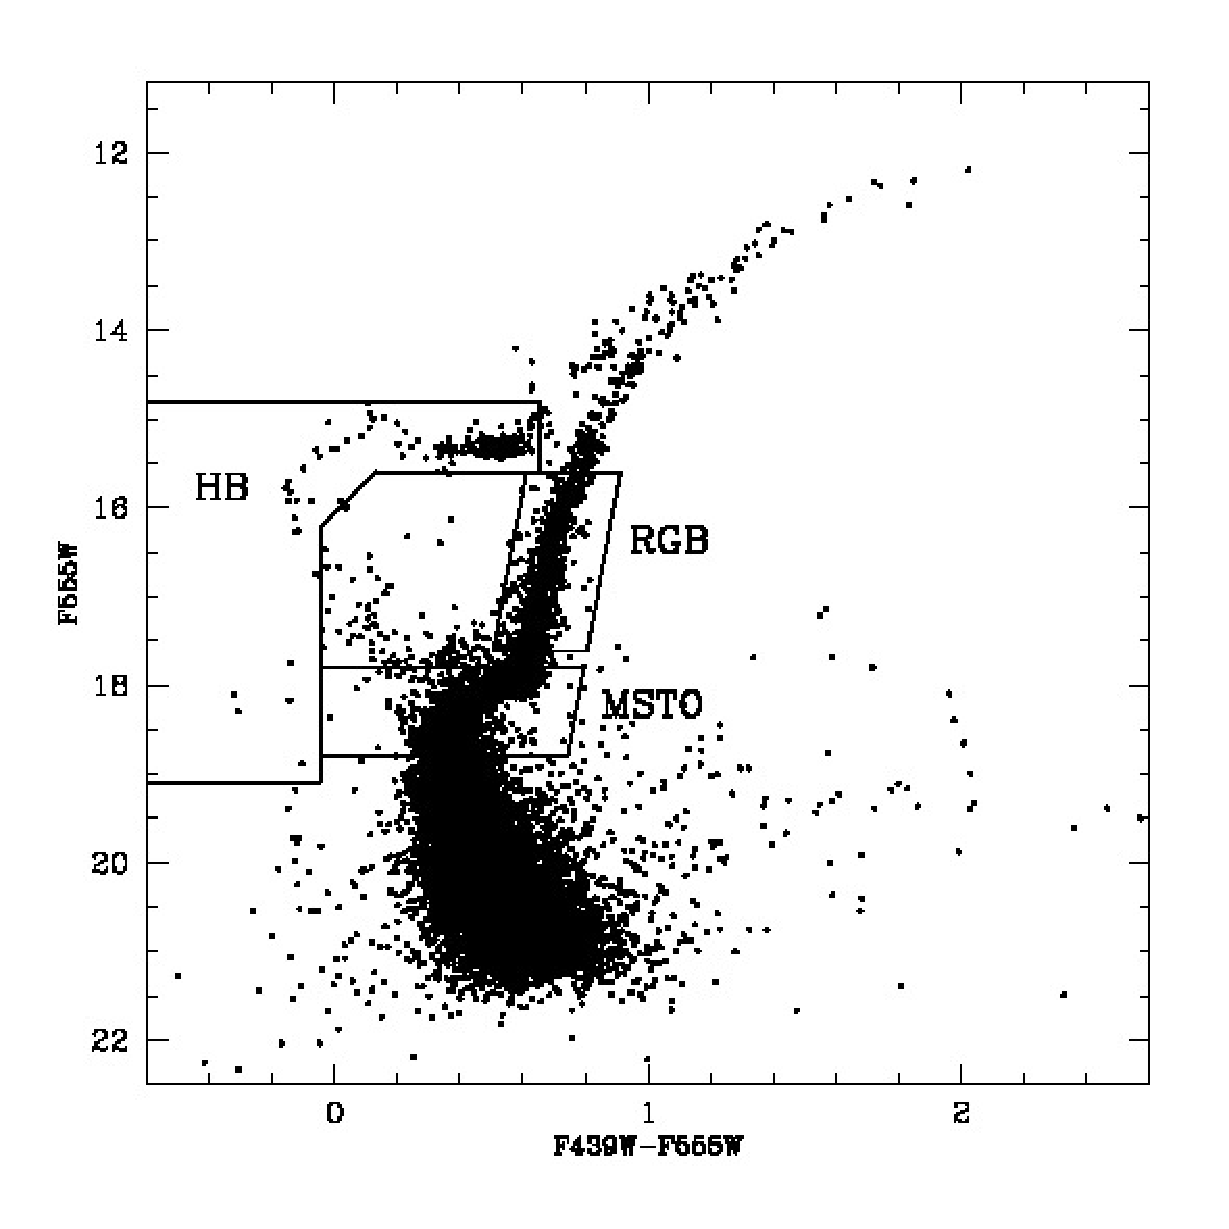
\includegraphics[scale=0.5]{Chapter-3/fig1.eps}
    \caption{Colour-magnitude diagram for
  NGC 362 in the (F439W-F555W)-F555W plane.  Boundaries enclosing the
  selected RGB, HB and MSTO populations are shown.  
    \label{fig:ngc0362_labels}}
  \end{center}
\end{figure}  

Errors on the number of stars for each stellar population were
calculated using Poisson statistics.  Core radii,  
distance moduli, extinction corrections, central luminosity
densities and central surface brightnesses were taken from the Harris
Milky Way Globular Cluster catalogue \citep{harris96}.  Calibrated
apparent magnitudes in the F555W, F439W and Johnson V bands 
were taken from \citet{piotto02}.

\section{Results} \label{results3}

This chapter focuses on the core RGB, MS and HB populations of 56
GCs, comparing their numbers to the core masses.  Note that we
are focusing on the total number of stars in the core as a proxy for the
core mass instead of the total luminosity in the core in order to
avoid concerns regarding cluster-to-cluster variations in the central
stellar mass function and selection effects.  Given that a single
bright HB star can be as luminous as 100 regular MS stars, 
a small surplus of bright stars could have a dramatic impact on
the total luminosity.  
Therefore, the total number of stars in
the core is a more direct and reliable estimate for the core mass than
is the core luminosity.

Upon plotting the logarithm of the number of core RGB stars
versus the logarithm of the total number of stars in the core and
performing a weighted least-squares fit, we find a relation of
the form:
\begin{equation}
\label{eqn:power-laws}
\log (N_{RGB}) = (0.89 \pm 0.03)\log (N_{core}/10^3) + (2.04 \pm 0.02)
\end{equation}
The sub-linear slope is either indicative of a surplus of RGB stars in the
least massive cluster cores or a deficiency in the most massive cores.
Errors for lines of best fit were  
found using a bootstrap methodology in which we generated 1,000 fake
data sets by randomly sampling (with replacement) RGB counts from the
observations.  We obtained lines of best fit for each fake data set, fit a
Gaussian to the subsequent distribution and extracted its standard
deviation.  In order to avoid the additional uncertainty introduced
into our RGB number counts from trying to distinguish AGB stars from RGB
stars, as well as the difficulty in creating a selection criterion that
is consistent from cluster-to-cluster when including the brightest
portion of the RGB, stars that satisfy the RGB 
selection criterion shown in Figure \ref{fig:ngc0362_labels} are
referred to as RGB stars throughout this chapter.  Note that it is
the brightest portion of the RGB that should be the most affected by
stellar evolution effects such as mass-loss.  If we
extend our selection criterion to include the entire RGB, however, our
results remain unchanged.

Interestingly, MS plus sub-giant branch stars (hereafter
collectively referred to as MSTO stars, the selection criterion for
which is shown in Figure 1) show a more linear relationship than do RGB
stars and appear to dominate the central star counts.  If we count
only those stars having a F555W mag within half a magnitude above and
below the turn-off, we obtain a relation of the form:
\begin{equation}
\log (N_{MSTO}) = (1.02 \pm 0.01)\log (N_{core}/10^3) + (2.66 \pm 0.01)
\end{equation}
A nearly identical fit is found when counting only those
stars having a F555W mag between the turn-off and one
magnitude fainter than the turn-off. 

We also tried plotting the logarithm of the number of core
helium-burning stars (labeled HB in Figure~\ref{fig:ngc0362_labels})
versus the logarithm of the number of stars in the core, yielding a
relation of the form:
\begin{equation}
\log (N_{HB}) = (0.91 \pm 0.10)\log (N_{core}/10^3) + (1.58 \pm 
0.05)
\end{equation}   
Note the large uncertainty associated with the fit, indicating that
the slope is consistent with both those of the RGB and MSTO samples.
We will discuss this stellar population further in
Section~\ref{discussion3}.

The number of MSTO, RGB and HB stars are shown as a function of the
total number of stars in the core in Figure \ref{fig:N_vs_ncore}.
Interestingly, the blue stragglers in our sample also scale
sub-linearly with core mass, albeit more dramatically, obeying a
relation of the form N$_{BS}$ $\sim$ M$_{core}^{0.38 \pm 0.04}$
\citep{knigge09}.  Note that N$_{core}$ can be used interchangeably
with M$_{core}$.  In this case, we obtain a fit of:
\begin{equation}
\label{eqn:power-law-bs}
\log (N_{BS}) = (0.47 \pm 0.06)\log (N_{core}/10^3) + (1.22 \pm 0.02)
\end{equation}

\begin{figure} [!h]
  \begin{center}
 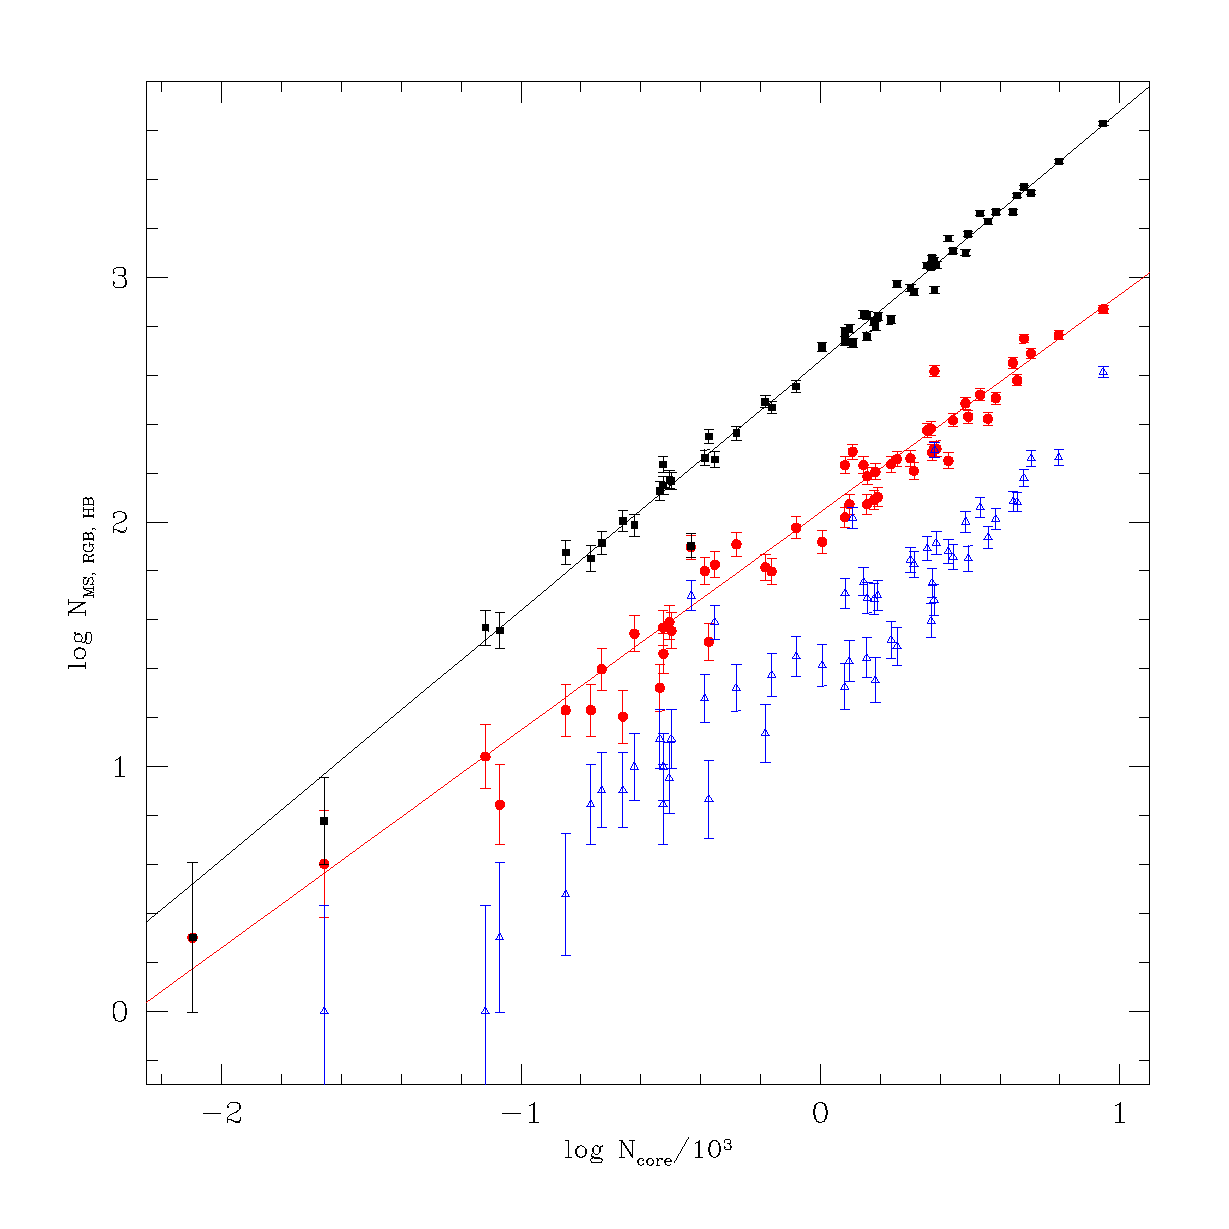
\includegraphics[scale=0.5]{Chapter-3/fig2.eps}
    \caption[N$_{core}$ versus N$_{MS,RGB,HB}$]{The number of RGB
  (red circles), MSTO (black squares) and HB (blue triangles) stars
  found within the cluster core plotted versus the total number of
  stars in the core brighter than 1 mag below the MSTO, along with the 
  corresponding lines of best fit for the RGB and MSTO samples.
    \label{fig:N_vs_ncore}}
  \end{center}
\end{figure}

In an effort to explore the influence of selection effects, we re-did our
plots having removed from our sample clusters denser than log $\rho$
$>$ 10$^5$ L$_{\odot}$ pc$^{-3}$ since we are the most likely to be
under-counting stars in the most crowded cluster cores where blending
of the stellar light is the most severe.  This cut also removes from
our sample the post-core collapse (PCC) clusters for which the core
radii are poorly defined since King models are known to provide a poor
fit to the observed surface brightness profiles in these clusters.
Similarly, we applied a cut in the central surface brightness,
removing from our sample clusters satisfying $\Sigma_0$ $<$ 15.1 V mag
arcsec$^{-2}$.  Finally, since clusters having both high surface
brightnesses and small cores are the most likely to suffer from
selection effects, we also tried adding to 
the aforementioned cut in $\Sigma_0$ a cut in the angular core radius,
removing clusters with r$_c$ $\le$ 0.05'.  In all cases, the
sub-linear power-law index reported for the RGB remains unchanged to
within one standard deviation of our original result.  Selection 
effects do not appear to be the source of the observed sub-linearity,
though it is clear that its effects must properly be accounted for in
future studies.

In order to assess the effects of age-related cluster-to-cluster
variations in the stellar mass function, as well as to test our
assumption that the number of stars in the core provides a reliable
estimate for the core mass, we have obtained MSTO 
masses for most of the GCs in our sample.  We fit theoretical
isochrones provided in \citet{pols98} to the cluster CMDs, using
the bluest point along the MS of a given isochrone as a proxy for the
MSTO mass.  Isochrones were calculated
using the metallicities of \citet{piotto02} and cluster ages were
taken from \citet{deangeli05} using the Zinn \& West (1984)
metallicity scale.  Core masses were estimated by multiplying the mass
corresponding to the MSTO (m$_{MSTO}$) by the number of stars in the
core brighter than 1 mag below the turn-off.  This is a reasonable
assumption given the very small dispersion in the ages of MW
GCs \citep{deangeli05} and the fact that we are only considering stars
brighter than 1 mag below the TO.  Consequently, the range of stellar
masses upon which we are basing our 
number counts is very small.  Our results remain entirely unchanged
upon using M$_{core}$ $\sim$ N$_{core}$m$_{MSTO}$ as a proxy for the
core mass instead of pure number counts.

In order to further check the sensitivity of our results to our estimate for
the core masses, we re-did all plots shown in
Figure~\ref{fig:N_vs_ncore} using various approximations for the total core
luminosity instead of pure number counts.  Core luminosities are
calculated in the Johnson V band directly from the stellar fluxes
which are summed over all stars in the core and then multiplied by the
appropriate geometric correction factor.  We also adopted L$_{core}$ =
$\frac{4}{3}\pi$r$_c^3$$\rho_0$, where $\rho_0$ is the
central luminosity density in L$_{\odot}$ pc$^{-3}$ taken from
\citet{harris96}.  Additionally, since the number of core RGB stars is
in reality a projected quantity, we tried plotting N$_{RGB}$ versus
L$_{core}$ = $\pi$r$_c^2$$\Sigma_0$, where 
$\Sigma_0$ is the central surface brightness in L$_{\odot}$ 
pc$^{-2}$, so that we are consistently comparing two projected
quantities.  Finally, we can adopt slightly more realistic
estimates for the total core luminosity by integrating over King
density profiles.  We fit single-mass King models calculated using the
method of \citet{sigurdsson95} to the surface brightness profiles of the
majority of the clusters in our sample using the concentration
parameters of \citet{mclaughlin05} and the central luminosity
densities of \citet{harris96}.  We then integrated the derived
luminosity density profiles numerically in order to estimate the total
stellar light contained within the core.  After removing clusters
labelled as post-core collapse in \citet{harris96} for which King
models are known to provide a poor fit, we once again compared the
integrated core luminosities to the number of RGB stars in the core.
For all four of these estimates for the total core luminosity, we
find that our fundamental results remain unchanged, with the power-law
index for RGB stars remaining sub-linear at the 3-$\sigma$ level.
Therefore, we conclude that our result is robust to changes in choices
of cluster and population parameters.  

\section{Discussion} \label{discussion3}

We have shown that the number of RGB stars in globular cluster cores
does not directly trace the total stellar population in those cores.  In
particular, the number of RGB (but not MSTO) stars 
scales sub-linearly with core mass at the 3-$\sigma$ level.  Given
that the MS lifetime is expected to be a factor of 10-100 
longer than that of the RGB sample \citep{iben91}, the ratio
N$_{MSTO}$/N$_{RGB}$ indicates that the relative sizes of these stellar
populations are in better agreement with the expectations of stellar evolution
theory in the most massive cores.  This suggests that our results are
consistent with a surplus of RGB stars in the least massive cores.  We 
discuss below some of the key considerations in understanding the
evolution of GC cores and the stars that populate them in an effort to
explain our result.

\subsection{Stellar evolution}

Could this trend be a reflection of a stellar evolution process?  The
evolution and distribution of stellar populations can be thought 
of as the sum of many single stellar evolution tracks, which depend
only on a star's mass and composition.  Since there is no relation
between a cluster's mass and its metallicity \citep{harris96} and the
dispersion in the relative ages of MW GCs is quite small
\citep{deangeli05}, there is no reason to expect the RGB 
lifetime to depend on the cluster mass.  On the other hand, recent
studies suggest that 
the chemical self-enrichment of GCs during their early evolutionary
stages could help to explain many of the population differences
observed among them \citep[e.g.][]{caloi07}.  In particular, many of
the most massive GCs are thought to be enriched in helium and this is
expected to reduce the time scale for stellar evolution
\citep[e.g.][]{romano07}.  While this scenario predicts a deficiency
of RGB stars in the most massive cores, it would contribute to
depressing the slope of the RGB sample relative to that of the MSTO
population in Figure~\ref{fig:N_vs_ncore}.  

\subsection{Single star dynamics} \label{dynamics3}

Two-body relaxation is the principal driving force behind the dynamical
evolution of present-day GCs, slowly steering them towards a state of
increased mass stratification as predominantly  
massive stars fall into the core and typically low-mass stars are
ejected via dynamical encounters.  The relaxation time increases
with the cluster mass \citep{spitzer87} and the variance in the relative ages
(and hence MSTO masses) of MW GCs is quite small
\citep{deangeli05}.  Therefore, it is the
least massive clusters that should show signs of being the
most dynamically evolved.  This assumes that cluster-to-cluster
variations in the initial mass function and the degree of
initial mass segregation are small.  In general, however,
proportionately fewer massive stars should have had sufficient time to
migrate into the most massive cores, while 
fewer low-mass stars should have been ejected out.  While qualitatively
correct, this effect should contribute little to the observed
difference between the core RGB and MSTO populations since RGB stars
are only slightly more massive \citep[e.g.][]{demarchi07}.

Stars expand considerably as they ascend the RGB.  Both the increase
in collisional cross-section and the change 
in the average stellar density could have an important bearing on the
outcomes of dynamical interactions involving RGB stars.  Indeed,
\citet{bailyn94} suggests that interactions between giants and other
cluster members in the core could strip the outer envelope of the
giant before it has a chance to fully ascend the RGB.  Since our
adopted RGB selection criterion does not include the brightest giants, 
we are only considering giants that are larger than MSTO stars
by a factor of $\sim$ 10 \citep{iben91}.  This small degree of
expansion will have only a minor effect on the collision rate.  Any
scenario that relies on dynamical encounters to explain a depletion of
RGB stars should be operating in very dense cores.  Our results are
consistent with some of the densest clusters in our sample having a
surplus of giants, however.  

\subsection{Binary effects}

Stripping of the envelopes of large stars could also be mediated by a
binary companion as the expanding giant overfills its Roche lobe
\citep{bailyn94}.  While this process should preferentially
occur in the centres of clusters where binaries will congregate as
a result of mass segregation, two-body relaxation progresses more
slowly in the most massive clusters.  Binaries should therefore sink 
to the cluster core more quickly in the least massive clusters,
contributing to an increase in the core binary fraction at a rate that
decreases with increasing cluster mass.  Observational evidence has
been found in support of this, most notably by \citet{sollima07} and
\citet{milone08} who found an anti-correlation between the cluster 
mass and the core binary fraction.  Any mechanism for RGB
depletion that relies on binary stars should therefore operate
more efficiently in the least massive cores where the binary
fraction is expected to be the highest.  Our results are consistent
with a surplus of giants in the least massive cores,
however.  This therefore argues against a binary mass-transfer origin
for RGB depletion in massive GC cores.  For similar reasons, it seems
unlikely that our result can be explained by collisions between RGB
stars and binaries.  If, on the other hand, 
RGB stars are more commonly found in binaries than are MS stars,
perhaps as a result of their larger cross-sections for tidal capture, 
binary stars could still be contributing to the observed trend.  Note
that in the cluster outskirts where the velocity dispersion has
dropped considerably from its central value, individual encounters are
more likely to result in tidal capture.  Since mass segregation should deliver
binaries to the core faster in the least massive clusters, a
larger fraction of their RGB stars could have hitched
a ride to the core as a binary companion.   However, both 
the average half-mass relaxation time of MW GCs and the RGB lifetime
tend to be on the order of a Gyr 
\citep{harris96, iben91}.  This does not leave much time for giants to be
captured into binaries and subsequently fall into the core before
evolving away from the RGB.

\subsection{Core helium-burning stars}

The fit for the HB sample is consistent with those of the RGB and MSTO
samples at the 3-sigma level so that we are unable to draw any
reliable conclusions for this stellar population.  The high
uncertainty stems from a number of outlying clusters.  
Selection effects and contamination from the Galaxy are likely to be
playing a role in this, in addition to our formulaic selection
criterion which may not be as suitable to the varying morphology of
the HB as it is to other stellar populations.  That is, the creation of
a purely photometry-based cluster-independent selection criterion may
not be possible for HB stars.  Given that stellar evolution effects
are expected to be the 
most dramatic at the end of the RGB lifetime, an interplay with the
cluster dynamics could also be contributing.  In particular, if the
central relaxation time is shorter than the HB lifetime, 
significant numbers of HB stars could be ejected from the core via
dynamical encounters as a result of having lost around a quarter of
their mass upon evolving off the tip of the RGB.  Moreover, since
stars expand considerably as they ascend the RGB, many of
the dynamical arguments presented in Section~\ref{dynamics3} may more
strongly affect the size of the HB sample if they are the direct
evolutionary descendants of RGB stars.  Since at most a handful of
studies have been performed comparing the radial HB and RGB
distributions in GCs \citep[e.g.][]{iannicola09}, more data is needed
before any firm constraints can be placed on the source of the 
poor fit found for the HB sample.

\subsection{An evolutionary link with blue stragglers?}

The addition of a small number of extra RGB stars to every cluster is one
way to account for the observed sub-linear dependence on core
mass since the fractional increase in the size of
the RGB population will be substantially larger in the least massive
cores.  In log-log space, the result is a reduction of the
slope.  Since blue stragglers will evolve
into RGB and eventually HB stars \citep{sills09}, evolved BSs could be
the cause of a surplus of RGB (and possibly  
core helium-burning) stars in these clusters.  This scenario also
predicts that MSTO stars should scale slightly more linearly with core
mass since there should be a smaller contribution from evolved BSs, as
we have shown.  Given the fits for the RGB and BS  
samples presented in Section~\ref{results3} and their corresponding
uncertainties, we find that the addition of evolved BSs to the RGB
populations could inflate the slope enough that the dependence on core
mass becomes linear.  Upon subtracting the BS sample from the RGB
sample, we find that the new fit is consistent with being linear:
\begin{equation}
\log (N_{RGB}) = (0.94 \pm 0.04)\log (N_{core}/10^3) + (1.97 \pm 0.02)
\end{equation}
The slope becomes larger if we have under-estimated the
number of BSs, perhaps as a result of selection effects, our adopted
selection criterion or a larger population size having existed in the
past.

\section{Summary} \label{summary3}

In this chapter, we have performed a cluster-to-cluster comparison
between the number of core RGB, MSTO \& HB stars 
and the total core mass.  We have introduced a technique for comparing
stellar populations in clusters that is well suited to studies of both
cluster and stellar evolution, in addition to the interplay thereof.
Using a sample of 56 GCs taken from Piotto et al.'s 2002 HST database,
we find a sub-linear scaling for RGB stars at the 3-$\sigma$ level,
whereas the relation is linear for MSTO stars.  While the preferential
self-enrichment of massive GCs, two-body relaxation, and evolved BSs
could all be contributing to the observed sub-linear dependence,
further studies with an emphasis on selection effects are needed in
order to better constrain the source of this curious observational result.

\section*{Acknowledgments}

We would like to thank an anonymous referee for a 
number of helpful suggestions, as well as Bill Harris, 
David Chernoff, Barbara Lanzoni and Francesco Ferraro for useful
discussions.  This research has been supported by NSERC as well as the
National Science Foundation under Grant No. PHY05-51164 to the Kavli
Institute for Theoretical Physics.

%\chapterbib

\begin{thebibliography}{99}
\bibitem[\protect\citeauthoryear{Bailyn}{1994}]{bailyn94} Bailyn,
  C. D. 1994, AJ, 107, 1073
\bibitem[\protect\citeauthoryear{Baumgardt \&
    Makino}{2003}]{baumgardt03} Baumgardt, H., \& Makino, J. 2003,
  MNRAS, 340, 227 
%\bibitem[\protect\citeauthoryear{Baumgardt et al.}{2008}]{baumgardt08}
%  Baumgardt, H., De Marchi, G., \& Kroupa, P. 2008, ApJ, 685, 247
\bibitem[\protect\citeauthoryear{Beer \& Davies}{2004}]{beer03} Beer,
  M. E. \& Davies, M. B. 2004, MNRAS, 348, 679
%\bibitem[\protect\citeauthoryear{Buonanno et al.}{1988}]{buonanno88}
%  Buonanno, R., Caloi, V., Castellani, V., Corsi, C. E., Ferraro,
%  I. \&  Piccolo, F. 1988, A\&AS, 74, 353
\bibitem[\protect\citeauthoryear{Caloi \& D'Antona}{2008}]{caloi08}
  Caloi, V. \& D'Antona, F. 2008, ApJ, 673, 847 
\bibitem[\protect\citeauthoryear{Caloi \& D'Antona}{2007}]{caloi07}
  Caloi, V. \& D'Antona, F. 2007, A\&A, 463, 949
\bibitem[\protect\citeauthoryear{De Angeli et al.}{2005}]{deangeli05}
  De Angeli, F., Piotto, G., Cassisi, S., Busso, G., Recio-Blanco, A.,
  Salaris, M., Aparicio, A., \& Rosenberg, A. 2005, AJ, 130, 116
\bibitem[\protect\citeauthoryear{De Marchi \& Pulone}{2007}]{demarchi07}
  De Marchi, G., \& Pulone, L. 2007, A\&A, 467, 107
%\bibitem[\protect\citeauthoryear{Ferraro et al.}{1991}]{ferraro91}
%  Ferraro, F. R. Clementi, G., Fusi Pecci, F., \& Buonanno, R. 1991,
%  MNRAS, 252, 357 
\bibitem[\protect\citeauthoryear{Harris}{1996}]{harris96}
  Harris, W. E. 1996, AJ, 112, 1487
\bibitem[\protect\citeauthoryear{Iannicola et al.}{2009}]{iannicola09}
  Iannicola, G., Monelli, M., Bono, G., Stetson, P. B., Buonanno, R.,
  Calamida, A., Zoccali, M., Caputo, F., Castellani, M., Corsi, C. E.,
  Dall'Ora, M., Cecco, A. Di, Deg'Innocenti, S., Ferraro, I., Nonino,
  M., Peitrinferni, A., Pulone, L., Moroni, P. G., Prada, R., M.,
  Sanna, N., \& Walker, A. R. 2009, ApJL, 696, L120
\bibitem[\protect\citeauthoryear{Iben}{1991}]{iben91} Iben, I.,
  Jr. 1991, ApJS, 76, 55
\bibitem[\protect\citeauthoryear{Knigge, Leigh \& Sills}{2009}]{knigge09}
  Knigge, C., Leigh, N., \& Sills, A. 2009, Nature, 457, 288
\bibitem[\protect\citeauthoryear{K\"upper et al.}{2008}]{kupper08}
  K\"upper, A. H. W., MacLeod, A., \& Heggie, D. C. 2008, MNRAS, 387,
  1248 
\bibitem[\protect\citeauthoryear{Lee et al.}{1994}]{lee94} Lee, Y.,
  Demarque, P., \& Zinn, R. 1994, ApJ, 423, 248
\bibitem[\protect\citeauthoryear{Leigh, Sills \& Knigge}{2007}]{leigh07} Leigh,
  N., Sills, A., Knigge, C. 2007, ApJ, 661, 210
\bibitem[\protect\citeauthoryear{Leigh, Sills \& Knigge}{2008}]{leigh08} Leigh,
  N., Sills, A., Knigge, C. 2008, ApJ, 678, 564
%\bibitem[\protect\citeauthoryear{McKee \& Ostriker}{2007}]{mckee07}
%  McKee, C. F., \& Ostriker, E. C. 2007, ARAA, 45, 565
%bibitem[\protect\citeauthoryear{McLaughlin}{2000}]{mclaughlin00}
% McLaughlin, D. E. 2000, MNRAS, 340, 227
\bibitem[\protect\citeauthoryear{McLaughlin \& van den
    Marel}{2005}]{mclaughlin05} McLaughlin, D. E., \& van der Marel,
  R. P. 2005, ApJS, 161, 304
\bibitem[\protect\citeauthoryear{Milone et al.}{2008}]{milone08}
  Milone, A. P., Piotto, G., Bedin, L. R., \& Sarajedini, A. 2008,
  MmSAI, 79, 623
\bibitem[\protect\citeauthoryear{Piotto et al.}{2002}]{piotto02}
  Piotto, G., King, I. R., Djorgovski, S. G., Sosin, C., Zoccali, M.,
  Saviane, I., De Angeli, F., Riello, M., Recio-Blanco, A., Rich,
  R. M., Meylan, G., \& Renzini, A. 2002, A\&A, 391, 945
\bibitem[\protect\citeauthoryear{Piotto et al.}{2004}]{piotto04}
  Piotto, G., De Angeli, F., King, I. R., Djorgovski, S. G., Bono, G.,
  Cassisi, S., Meylan, G., Recio-Blanco, A., Rich, R. M., \& Davies,
  M. B. 2004, ApJL, 604, L109 
\bibitem[\protect\citeauthoryear{Pols et al.}{1998}]{pols98} Pols,
  O. R., Schroder, K., Hurley, J. R., Tout, C. A., \& Eggleton,
  P. P. 1998, MNRAS, 298, 525
\bibitem[\protect\citeauthoryear{Romano et al.}{2007}]{romano07}
  Romano, D., Matteucci, F., Tosi, M., Pancino, E., Bellazzini, M.,
  Ferraro, F. R., Limongi, M., \& Sollima, A. 2007, MNRAS, 376, 405
\bibitem[\protect\citeauthoryear{Sandquist \&
    Martel}{2007}]{sandquist07} Sandquist, E. L. \& Martel,
  A. R. 2007, ApJ, 654, L65 
\bibitem[\protect\citeauthoryear{Sandquist \&
    Hess}{2008}]{sandquist08} Sandquist, E. L. \& Hess, J. M. 2008,
  AJ, 136, 2259 
\bibitem[\protect\citeauthoryear{Sigurdsson \&
    Phinney}{1995}]{sigurdsson95} Sigurdsson, S. \& Phinney,
  E. S. 1995, ApJS, 99, 609 
\bibitem[\protect\citeauthoryear{Sills et al.}{2009}]{sills09} Sills,
  A., Karakas, A., \& Lattanzio, J. 2009, ApJ, 692, 1411
\bibitem[\protect\citeauthoryear{Sollima et al.}{2007}]{sollima07}
  Sollima, A., Beccari, G., Ferraro, F. R., Fusi Pecci, F., \&
  Sarajedini, A. 2007, MNRAS, 380, 781
\bibitem[\protect\citeauthoryear{Spitzer}{1987}]{spitzer87} Spitzer,
  L. 1987, Dynamical Evolution of Globular Clusters (Princeton:
  Princeton University Press)
\bibitem[\protect\citeauthoryear{Zinn}{1984}]{zinn84} Zinn, R. \& West,
  M. J. 1984, ApJS, 55, 45
\end{thebibliography}

%\bsp

%\label{lastpage}

%\end{document}

\pagestyle{fancy}
\headheight 20pt
\lhead{Ph.D. Thesis --- K. Sliwa }
\rhead{McMaster - Physics \& Astronomy}
\chead{}
\lfoot{}
\cfoot{\thepage}
\rfoot{}
\renewcommand{\headrulewidth}{0.1pt}
\renewcommand{\footrulewidth}{0.1pt}
\setlength{\epigraphwidth}{5.in}
\chapter{Around the Ring We Go: The Cold, Dense Ring of Molecular Gas in NGC 1614} \label{chapter2} 
\thispagestyle{fancy} 

\linespread{1.5}
\epigraph{%\vspace{1.5in}
\normalsize \textit{``Theories crumble, but good observations never fade.''}}
  {\normalsize \textsc{\\ Harlow Shapley} (1885 - 1972)}
  
  asfa
%Gravity is the glue that holds our Universe together.  It binds the
%gas that forms stars, and is the reason they are rarely found 
%alone. 
%
%One is the lonesliest number.  Thanks to gravity, however, this
%expression rarely applies to stars.  
%\bsp

%\label{lastpage}

%\end{document}
\pagestyle{fancy}
\headheight 20pt
\lhead{Ph.D. Thesis --- N. Leigh }
\rhead{McMaster - Physics \& Astronomy}
\chead{}
\lfoot{}
\cfoot{\thepage}
\rfoot{}
\renewcommand{\headrulewidth}{0.1pt}
\renewcommand{\footrulewidth}{0.1pt}

%\chapter{Introduction} \label{chapter1}
%\thispagestyle{fancy}

%Latex Template
%Astronomy 3Y03
%Alison Sills
%Version 1.0 November 2005

%Do not change these three lines

\chapter{An Analytic Model for
  Blue Straggler Formation in Globular Clusters} \label{chapter5}
%%%\author[Nathan Leigh and Alison Sills]{Nathan Leigh$^{1}$,
%%%  Alison Sills$^{1}$\thanks{E-mail: leighn@mcmaster.ca (NL);
%%%    asills@mcmaster.ca (AS)} \\
%%%$^{1}$Department of Physics and Astronomy, McMaster University,
%%%1280 Main St. W., Hamilton, ON, L8S 4M1, Canada}
%%%\begin{document}
%
\thispagestyle{fancy}

\section{Introduction} \label{intro5}

Commonly found in both open and globular clusters (GCs), blue
stragglers (BSs) appear as an
extension of the main-sequence (MS) in cluster colour-magnitude
diagrams (CMDs), occupying the region that is just brighter and bluer
than the main-sequence turn-off (MSTO) 
\citep{sandage53}.  BSs are
thought to be produced via the addition of hydrogen to 
low-mass MS stars \citep[e.g.][]{sills01, lombardi02}.  This can
occur via multiple channels, most of which involve the mergers of
low-mass MS stars since a significant amount of mass is typically
required to reproduce the observed locations of BSs in CMDs
\citep[e.g.][]{sills99}.  Stars in close binaries can merge if enough
orbital angular momentum is lost, which can be mediated by dynamical
interactions with other stars, magnetized stellar winds, tidal
dissipation or even an outer triple companion
\citep[e.g.][]{leonard92, li06, perets09, dervisoglu10}.
Alternatively, MS stars can collide directly, although this is
also thought to usually be mediated by multiple star systems
\citep[e.g.][]{leonard89, leonard95, fregeau04, leigh11b}.  First proposed by
\citet{mccrea64}, BSs have also been hypothesized to form by
mass-transfer from an evolving primary onto a normal MS companion
via Roche lobe overflow.

Despite numerous formation
mechanisms having been proposed, a satisfactory explanation to account
for the presence of BSs in star clusters eludes us still.  Whatever the
dominant BS 
formation mechanism(s) operating in dense clusters, it is now
thought to somehow involve multiple star systems.  This was shown
to be the case in even the dense cores of GCs \citep{leigh07, leigh08,
  knigge09} where
collisions between single stars are thought to occur frequently
\citep{leonard89}.  In \citet{knigge09}, we showed that the numbers of
BSs in the cores
of a large sample of GCs correlate with the core masses.  We
argued that our results are consistent with what is expected if BSs
are descended from binary stars since this would imply a dependence of
the form $N_{BS} \sim f_bM_{core}$, where $N_{BS}$ is the number of
BSs in the core, $f_b$ is the binary fraction in the core and
$M_{core}$ is the total stellar mass contained within the core.
\citet{mathieu09} also showed 
that at least $76\%$ of the BSs in the old open cluster NGC 188 have
binary companions.  Although the nature of these companions remains
unknown, it is clear that binaries played a role in the
formation of these BSs.  

Blue stragglers are typically concentrated in the dense cores of
globular clusters where the high 
stellar densities should result in a higher rate of stellar encounters 
\citep[e.g.][]{leonard89}.  Whether or not this fact is
directly related to BS formation remains unclear, since mass segregation 
also acts to migrate BSs (or their progenitors) into the core 
\citep[e.g.][]{saviane98, guhathakurta98}.  Additionally, numerous BSs
have been observed in more sparsely populated open clusters
\citep[e.g.][]{andrievsky00} and the fields of GCs where
collisions are much less likely to occur and mass-transfer within
binary systems is thought to be a more likely formation scenario
\citep[e.g.][]{mapelli04}.  

Several studies have provided evidence
that BSs show a bimodal spatial distribution in some GCs
\citep{ferraro97, ferraro99, lanzoni07}.  In these clusters, the BS
numbers are the highest in the central cluster 
regions and decrease with increasing distance from the cluster centre
until a second rise occurs in the cluster outskirts.  
This drop in BS numbers at intermediate cluster radii is often
referred to as the ``zone of avoidance''.  Some authors have suggested
that it is the result of two separate formation mechanisms
occurring in the inner and outer regions of the cluster, with
mass-transfer in primordial binaries dominating in the latter and
stellar collisions dominating in the former
\citep{ferraro04, mapelli06}.  Conversely, mass segregation could also
give rise to a ``zone of avoidance'' for BSs if the time-scale for dynamical
friction exceeds the average BS lifetime in only the outskirts of GCs that
exhibit this radial trend \citep[e.g.][]{leigh11a}. 

Dynamical interactions occur frequently enough in dense clusters that
they are expected to be at least partly responsible for the observed
properties of BSs \citep[e.g.][]{stryker93, leigh11b}.  It follows
that the current properties of BS populations
should reflect the dynamical histories of their host clusters.  As a
result, BSs could provide an indirect means of probing
the physical processes that drive star cluster evolution
\citep[e.g.][]{heggie03, hurley05, leigh11b}.

In this chapter, our
goal is to constrain the dominant BS formation mechanism(s) operating
in the dense cores of GCs by analyzing the principal processes
thought to influence their production.  To this end, we
use an analytic treatment to obtain predictions for the number of BSs
expected to be found within one core radius of the cluster centre at
the current cluster age.  Predicted numbers for the core are calculated
for a range of free parameters, and then compared to the
observed numbers in order to find the
best-fitting model parameters.  In this way, we are able to quantify
the degree to which each of the considered formation mechanisms
should contribute to the total predicted numbers in order to
best reproduce the observations.  

In Section~\ref{data5}, we describe the BS catalogue used for comparison
to our model predictions.  In 
Section~\ref{method5}, we present our analytic model for BS 
formation as well as the statistical technique we have developed to
compare its predictions to the observations.  
These predictions are then compared to the observations in
Section~\ref{results5} for a range of model parameters.  In
Section~\ref{discussion5}, we discuss the implications of our results
for BS formation, as well as the role played by the cluster dynamics
in shaping the current properties of BS populations.

\section{The Data} \label{data5}

The data used in this study was taken from \citet{leigh11a}.  In that 
chapter, we presented a catalogue for blue straggler, red giant branch
(RGB), horizontal branch (HB) and main-sequence turn-off stars
obtained from the colour-magnitude diagrams of 35 Milky Way GCs
taken 
from the ACS Survey for Globular Clusters \citep{sarajedini07}.  The
ACS Survey provides unprecedented deep photometry in the F606W ($\sim$
V) and F814W ($\sim$ I) filters
that extends reliably from the HB all the way down to about 7
magnitudes below the MSTO.  The clusters in our sample span a range of
total masses (by nearly 3 orders of magnitude) and central
concentrations \citep{harris96}.  We have confirmed that 
the photometry is nearly complete in the BS region of the CMD for
every cluster in our sample.  This was 
done using the results of artificial star tests taken from
\citet{anderson08}.

Each cluster was centred in the ACS field, which 
extends out to several core radii from the cluster
centre in most of the clusters in our sample.  Only the core
populations provided in \citet{leigh11a} are used in this chapter.
We have taken estimates for the core radii and central luminosity
densities for the clusters in our sample from
\citet{harris96}, whereas central velocity 
dispersions were taken from \citet{webbink85}.  Estimates for the
total stellar mass contained within the core were obtained from
single-mass King models, as described in \citet{leigh11a}.  All of the
clusters in our sample were chosen to be non-post-core collapse, and
have surface brightness profiles that provide good fits to our King
models. 

\section{Method} \label{method5}

In this section, we present our model and outline our
assumptions.  We also present the statistical technique used to
compare the 
observed number counts to our model predictions in order to identify
the best-fitting model parameters. 

\subsection{Model} \label{model5}

Consider a GC core that is home to N$_{BS,0}$ BSs at some time t $=$
t$_0$.  At a specified time in the future, the number of BSs in the
core can be approximated by: 
\begin{equation}
\label{eqn:number-bss}
N_{BS} = N_{BS,0} + N_{coll} + N_{bin} + N_{in} - N_{out} - N_{ev},
\end{equation}
where N$_{coll}$ is the number of BSs formed from collisions during
single-single (1+1), single-binary (1+2) and binary-binary (2+2)
encounters, N$_{bin}$ is the number formed from 
binary evolution (either partial mass-transfer between the binary
components or their complete coalescence), N$_{in}$ is the number 
of BSs that migrate into the core due to dynamical friction, N$_{out}$
is the number that migrate out of the core via kicks experienced during
dynamical encounters, and N$_{ev}$ is the number of BSs that have
evolved away from being brighter and bluer than the MSTO in the
cluster CMD due to stellar evolution.  

We adopt an average stellar mass of $m = 0.65 M_{\odot}$ and an
average BS mass of $m_{BS} = 2m = 1.3 M_{\odot}$.  The mass of a BS
can provide a rough guide to its lifetime, although a range of
lifetimes are still possible for any given mass.  
For instance, \citet{sandquist97} showed that a
1.3 M$_{\odot}$ blue straggler will have a lifetime of around $0.78$
Gyrs in unmixed models, or 1.57 Gyrs in 
completely mixed models.  Combined with the results of \citet{sills01},
\citet{lombardi02} and \citet{glebbeek08}, we expect a lifetime in the
range 1-5 Gyrs for a 1.3 M$_{\odot}$ BS.  As a first approximation, we
choose a likely value of $\tau_{BS} = 1.5$ Gyrs for the average BS
lifetime \citep[e.g.][]{sills01}.  The effects had on our
results by changing our assumption for the average BS lifetime will be
explored in Section~\ref{results5} and discussed in
Section~\ref{discussion5}. 

We consider only the last $\tau_{BS}$ years.  This is because we are
comparing our model predictions to current
observations of BS populations, so that we are only concerned with
those BSs formed within the last few Gyrs.  Any BSs formed before this
would have evolved away from being brighter and bluer than the MSTO by
the current cluster age.  Consequently, we set N$_{BS,0}$ =
N$_{ev}$ in Equation~\ref{eqn:number-bss}.  We further assume that
all central cluster parameters have not changed in the last
$\tau_{BS}$ years, including the central velocity dispersion, the
central luminosity density, the core radius and the core binary
fraction.  It follows that the rate of BS formation is constant for
the time-scale of interest.  This time-scale is
comparable to the half-mass relaxation time but much longer than the
central relaxation time for the majority of the clusters in our sample
\citep{harris96}.  This suggests that core
parameters such as the central density and the core radius will
typically change in a time $\tau_{BS}$ since the time-scale on
which these parameters vary is the central relaxation
time \citep{heggie03}.  Therefore, our assumption of constant rates
and cluster parameters is not strictly correct, however it provides a
suitable starting point for our model.  We will discuss the
implications of our assumption of time-independent cluster properties
and rates in Section~\ref{discussion5}.

In the following sections, we discuss each of the remaining terms in
Equation~\ref{eqn:number-bss}.

\subsubsection{Stellar Collisions} \label{collisions5}

We can approximate the number of BSs formed in the last $\tau_{BS}$
years from collisions during dynamical encounters as:  
\begin{equation}
\label{eqn:number-coll}
N_{coll} = f_{1+1}N_{1+1} + f_{1+2}N_{1+2} + f_{2+2}N_{2+2},
\end{equation}
where N$_{1+1}$, N$_{1+2}$ and N$_{2+2}$ are the number of
single-single, single-binary and binary-binary encounters,
respectively.  The terms f$_{1+1}$, f$_{1+2}$ and f$_{2+2}$ are the
fraction of 1+1, 1+2 and 2+2 encounters, respectively, that will
produce a BS in the last $\tau_{BS}$ years.  We treat these three
variables as free parameters since we do not know what fraction of
collision products will produce BSs (i.e. stars with an appropriate
combination of colour and brightness to end up in the BS region of the
CMD), nor do we know what fraction of 1+2 and 2+2 encounters will
result in a stellar collision.  Numerical scattering experiments have
been performed to study the outcomes of 1+2 and 2+2 encounters
\citep[e.g.][]{hut83, mcmillan86, fregeau04}, however a large fraction
of the relevant parameter space has yet to be explored.

In terms of the core radius $r_c$ (in parsecs), the central number
density $n_0$ (in pc$^{-3}$), the root-mean-square velocity $v_{m}$
(in km s$^{-1}$), the average stellar mass $m$ (in M$_{\odot}$) and
the average stellar radius $R$ (in R$_{\odot}$), the mean time-scale
between single-single collisions in the core of a GC is
\citep{leonard89}:
\begin{equation}
\begin{gathered}
\label{eqn:coll1+15}
\tau_{1+1} = 1.1 \times 10^{10}(1-f_b)^{-2} \Big(\frac{1 pc}{r_c}
\Big)^3 \Big(\frac{10^3 pc^{-3}}{n_0} \Big)^2 \\
 \Big(\frac{v_{m}}{5
  km/s} \Big) \Big(\frac{0.5 M_{\odot}}{m} \Big) \Big(\frac{0.5
  R_{\odot}}{R} \Big)\mbox{ years}
\end{gathered}
\end{equation}
The additional factor (1-f$_b$)$^{-2}$ comes from the fact that we
are only considering interactions between single stars and the
central number density of single stars is given by (1-f$_b$)n$_0$,
where f$_b$ is the binary fraction in the core (i.e. the fraction of
objects that are binaries).  For our chosen mass, we assume a
corresponding average stellar radius using the relation M/M$_{\odot}$
= R/R$_{\odot}$ \citep{iben91}.
The number of 1+1 collisions expected to have occurred in the last
$\tau_{BS}$ years is then approximated by:
\begin{equation}
\label{eqn:N-1+1}
N_{1+1} = \frac{\tau_{BS}}{\tau_{1+1}}.
\end{equation}

The rate of collisions
between single stars and binaries, as well as between two
binary pairs, can be roughly approximated in the same way
as for single-single encounters \citep{leonard89, sigurdsson93,
  bacon96, fregeau04}.  We adopt the time-scales derived in
\citet{leigh11b} for the average times between 1+2 and 2+2 encounters.
These are:
\begin{equation}
\begin{gathered}
\label{eqn:coll1+25}
\tau_{1+2} = 3.4 \times 10^7f_b^{-1}(1-f_b)^{-1}\Big(\frac{1 pc}{r_c}
\Big)^3 \Big(\frac{10^3 pc^{-3}}{n_0} \Big)^2 \\
 \Big(\frac{v_{m}}{5
  km/s} \Big) \Big(\frac{0.5 M_{\odot}}{m} \Big) \Big(\frac{1 AU}{a}
\Big)\mbox{ years}
\end{gathered}
\end{equation}
and
\begin{equation}
\begin{gathered}
\label{eqn:coll2+25}
\tau_{2+2} = 1.3 \times 10^7f_b^{-2}\Big(\frac{1 pc}{r_c}
\Big)^3 \Big(\frac{10^3 pc^{-3}}{n_0} \Big)^2 \\ 
\Big(\frac{v_{m}}{5
  km/s} \Big) \Big(\frac{0.5 M_{\odot}}{m} \Big) \Big(\frac{1 AU}{a}
\Big)\mbox{ years},
\end{gathered}
\end{equation}
where $a$ is the average binary semi-major axis in the core in AU and
we have assumed that the average binary mass is equal to twice the
average single star mass.  
The numbers of 1+2 and 2+2 encounters expected to have occurred in the 
last $\tau_{BS}$ years are given by, respectively:
\begin{equation}
\label{eqn:N-1+2}
N_{1+2} = \frac{\tau_{BS}}{\tau_{1+2}}
\end{equation}
and
\begin{equation}
\label{eqn:N-2+2}
N_{2+2} = \frac{\tau_{BS}}{\tau_{2+2}}.
\end{equation}

The outcomes of 1+2 and 2+2 encounters will ultimately contribute to
the evolution of the binary fraction in the core.  How and with what
frequency binary 
hardening/softening as well as capture, exchange and ionization
interactions affect the binary fraction in the dense cores of GCs is
currently a subject of debate \citep[e.g.][]{ivanova05,
  hurley07}.  
Observations are also lacking for binary fractions in the dense cores of
GCs, however rough constraints suggest that they range from a few to a
few tens of a percent \citep[e.g.][]{rubenstein97, cool02, sollima08,
  davis08}.  The 
situation is even worse for the distribution of binary orbital
parameters observed in dense stellar environments.  Our best
constraints come from radial velocity surveys of moderately dense open
clusters \citep{latham05, geller09}, however whether or not the
properties of the binary populations in these clusters should differ
significantly from those in the much denser cores of GCs is unclear.
As an initial assumption, we assume a time-independent core binary
fraction of 10\% for all clusters, and an average semi-major axis
of 2 AU.  This semi-major axis corresponds roughly to the hard-soft
boundary for most of the clusters in our sample, defined by setting
the average binary orbital energy equal to the kinetic energy of an
average star in the cluster \citep[e.g.][]{heggie03}.  We 
treat both the core binary 
fraction and the average binary semi-major axis as free parameters,
and explore a range of possibilities using the available observations
as a guide for realistic values.  We will return to these assumptions 
in Section~\ref{discussion5}.

\subsubsection{Binary Star Evolution} \label{mergers5}

Although we do not know the rate of BS formation from binary star
evolution, we expect a general relation of the form
N$_{bin}$ = $\tau_{BS}$/$\tau_{mt}$ for the number of BSs produced
from binary mergers in the last $\tau_{BS}$ years, where $\tau_{mt}$
is the average time between BS formation events due to binary star
evolution.  We can express the number of BSs formed from binary star
evolution in the last $\tau_{BS}$ years as:
%, which is inversely
%proportional to $\tau_{mt}$, as:
%rate of BS formation from binary star
%evolution, which is inversely proportional to $\tau_{mt}$, as
%f$_{mt}$f$_b$N$_{core}$, where  N$_{core}$ is the total number of
%objects (i.e. single and binary stars) in the core and f$_{mt}$ is
%the fraction of binary stars that evolved internally to form
%BSs within the last $\tau_{BS}$ years.  This gives:
\begin{equation}
\label{eqn:N-bin}
N_{bin} = f_{mt}f_bN_{core},
\end{equation}
where  N$_{core}$ is the total number of
objects (i.e. single and binary stars) in the core and f$_{mt}$ is
the fraction of binary stars that evolved internally to form
BSs within the last $\tau_{BS}$ years.  We treat f$_{mt}$ as a free
parameter since it is likely to depend on the mass-ratio, period and
eccentricity distributions characteristic of the binary populations of
evolved GC cores, for which data is scarce at best.  

\subsubsection{Migration Into and Out of the Core}
\label{segregation5}

Due to the relatively small sizes of the BS populations
considered, the migration of BSs into or out of the core is an
important consideration when calculating the predicted numbers.  In
other words, we are dealing with relatively small
number statistics and every blue straggler counts.  In order to
approximate the number of stars in the core as a function of time,
two competing effects need to be taken into account:  (1) mass
stratification/segregation (or, equivalently, dynamical friction) and
(2) kicks experienced during dynamical interactions.  
These effects are accounted for with the variables N$_{in}$ and
N$_{out}$ in Equation~\ref{eqn:number-bss}, respectively.  

Blue stragglers are among the most massive stars in clusters
\citep[e.g.][]{shara97, vandenberg01, mathieu09}, so they should
typically be heavily mass segregated relative to other stellar
populations \citep[e.g.][]{spitzer69, shara95, king95}.  The
time-scale for this process to occur 
can be approximated using the dynamical friction time-scale \citep{binney87}:
\begin{equation}
\label{eqn:t-dyn}
\tau_{dyn} = \frac{3}{4ln{\Lambda}G^2(2{\pi})^{1/2}}\frac{\sigma(r)^3}{m_{BS}\rho(r)},
\end{equation}  
where $\sigma(r)$ and $\rho(r)$ are, respectively, the velocity
dispersion and stellar mass density at the given distance from the
cluster centre $r$.  Both $\sigma(r)$ and $\rho(r)$ are found from
single-mass King models \citep{sigurdsson93}, which are fit to each
cluster using the 
concentration parameters provided in \citet{mclaughlin05}.  
The Coulomb logarithm is denoted by $\Lambda$, and we adopt
a value of ln$\Lambda \sim 10$ throughout this chapter 
\citep[e.g.][]{spitzer87, heggie03}.  If $\tau_{dyn} >
\tau_{BS}$ at a given distance from the 
cluster centre, then any BSs formed at this radius in the last
$\tau_{BS}$ years will not have had sufficient time to migrate into
the core by the current 
cluster age.  The maximum radius r$_{max}$ at which BSs can
have formed in the 
last $\tau_{BS}$ years and still have time to migrate into the core
via dynamical friction is given by setting $\tau_{dyn} = \tau_{BS}$.  
Therefore, N$_{in}$ depends only on the number of BSs formed in the last
$\tau_{BS}$ years at a distance from the cluster centre smaller than
r$_{max}$.  

In order to estimate the contribution to N$_{BS}$ in
Equation~\ref{eqn:number-bss} from BSs formed outside the core, we
calculate the number of BSs formed in radial shells between the
cluster centre and r$_{max}$.  Each shell is taken to be one core
radius thick, and we calculate the contribution from 
each formation mechanism in every shell.  This is done by assuming a
constant (average) density and velocity dispersion in each shell.
Specifically, we estimated the density and velocity 
dispersion at the half-way point in each shell using our single-mass King models,
and used these to set average values.  The number of BSs expected to
have migrated into the core within the last $\tau_{BS}$ years can be
written:
\begin{equation}
\begin{gathered}
\label{eqn:N-in}
N_{in} = \sum_{i=2}^N \Big( f_{1+1}N_{(1+1),i} + f_{1+2}N_{(1+2),i} +
f_{2+2}N_{(2+2),i} \\ 
+ f_{mt}N_{(bin),i} \Big) \times \Big(1 -
\frac{\tau_{(dyn),i}}{\tau_{BS}}\Big),
\end{gathered}
\end{equation}
where $i=1$ refers to the core, $i=2$ refers to the shell immediately 
outside the core, etc. and N is taken to be the integer nearest to
r$_{max}$/r$_c$.  We let the terms with N$_{(1+1),i}$, N$_{(1+2),i}$,
N$_{(2+2),i}$ and 
N$_{(bin),i}$ represent the number of BSs formed in shell $i$ from
single-single collisions, single-binary collisions, binary-binary
collisions and binary star evolution, respectively.  The time-scale
for dynamical friction in shell $i$ is denoted by $\tau_{(dyn),i}$, and
the factor (1 - $\tau_{(dyn),i}$/$\tau_{BS}$) is included to account for
the fact that we are assuming a constant formation rate for BSs, so
that not every BS formed in shells outside the core will have
sufficient time to fall in by the current cluster age.

It is typically the least massive stars
that are ejected from 1+2 and 2+2 interactions as single stars
\citep[e.g.][]{sigurdsson93}.  Combined with conservation of momentum,
this suggests that BSs are the least likely to be ejected from
dynamical encounters with velocities higher than the central velocity
dispersion due to their large masses.  This has been confirmed by
several studies of numerical scattering experiments 
\citep[e.g.][]{hut83, fregeau04}.  Based on this, we 
expect that N$_{out}$ should be 
very small and so, as a first approximation, we take N$_{out} = 0$.
However, we also explore the effects of a 
non-zero N$_{out}$ by assigning a kick velocity to all BSs at birth.
If dynamical interactions play a role in BS formation, we 
might naturally expect BSs to be imparted a recoil velocity at birth
(or shortly before) due to 
momentum conservation.  We will return to this assumption in
Section~\ref{results5}. 

\subsection{Statistical Comparison with Observations} \label{statistics5}

Our model contains 4 free parameters, which correspond to the fraction of
outcomes that produce a blue straggler for each formation mechanism
(1+1 collisions, 1+2 collisions, 2+2 collisions, and binary star
evolution).  These are the $f$ values
described in the previous section: $f_{1+1}, f_{1+2}, f_{2+2},
f_{mt}$.  We assume that these values are constant throughout each
cluster, and are also constant between clusters.  By fitting the
predictions of our model to the observational data, we can determine
best-fit values for each of these $f$ parameters, and therefore make
predictions about which blue straggler formation processes are
more important. 

In order to determine the best values for these $f$ parameters, we 
need an appropriate statistical test.  For this, we follow the approach
of \citet{verbunt08}.  The number of BSs seen in the core of
a globular cluster can be described by Poisson statistics.  In
particular, the probability of observing $N$ sources when $\mu$ are
expected is:
\begin{equation}
\label{eqn:stats5}
P(N,\mu) = \frac{\mu^N}{N!}e^{-\mu}
\end{equation}
We can calculate a probability for each cluster, and then calculate an 
overall probability $P^{\prime}$ for the model by multiplying the
individual $P$ values.  We can then vary the $f$ values to maximize
this value. 

In practice, these $P$ values are typically of order ten percent per
cluster, and with 35 clusters, the value of $P^{\prime}$ quickly
becomes extremely small.  Therefore we chose to work with a modified
version of this value:  the deviance of our model to the saturated
model.  A saturated model is one in which the observed number of
sources is exactly equal to the expected number in each cluster.  In
other words, this is the best that we can possibly do.  However,
because of the nature of Poisson statistics, the probability $P$ of
such a model (calculated by setting $N=\mu$ in
Equation~\ref{eqn:stats5}) is not equal to 1, but in fact has some
smaller value.  For the numbers of blue stragglers in our clusters,
the $P$ values for the saturated model run from 0.044 to 0.149, and
the value of $P^{\prime}$ is $2.08 \times 10^{-41}$.

The deviance of any model from the saturated model is given by
\begin{equation}
\label{eqn:deviance}
D = 2.0(\ln(P^{\prime}_{saturated}) - \ln(P^{\prime}_{model}))
\end{equation}
The model which minimizes this quantity will be our best-fit
model.  Ideally, the scaled deviance ($D/(N_{data}-N_{parameters}$)
should be equal to 1 for a best fit.  Given the simplicity of our
model, we expect that our values will not provide this kind of
agreement, and we simply look for the model which provides the minimum
of the scaled deviance.

\section{Results} \label{results5}

In this section, we present the results of comparing our model
predictions to the observations.  After presenting the results for 
a constant core binary fraction for all clusters, we explore the
implications of adopting a core binary fraction that depends on the
cluster luminosity, as reported in \citet{sollima07} and
\citet{milone08}. 

\subsection{Initial Assumptions} \label{initial}

The predictions of our model for our initial choice of assumptions are
shown in Figure~\ref{fig:model_best}.  These numbers are plotted
against the total stellar mass in the core along with the 
number of BSs observed in the core (blue triangles).  We plot both the
total number of BSs predicted to have formed within $r_{max}$ in the
last $\tau_{BS}$ years (N$_{BS}$ in Equation~\ref{eqn:number-bss};
green circles), as well as the total number formed only in the core
(N$_{coll}$ + N$_{bin}$; red circles).  Upon comparing N$_{BS}$ to the
observed number of BSs in the core, 
the best-fitting model parameters predict that most BSs are formed
from binary star evolution, with a small contribution from 2+2
collisions being needed in order to obtain the best possible match to
the observations.  The ideal contribution from 2+2 collisions
constitutes at 
most a few percent of the predicted total for most of the clusters in
our sample.  Even for our best-fitting model
parameters, our initial choice of assumptions predicts too few BSs in
clusters with small core masses. 

\begin{figure} [!h]
  \begin{center}
 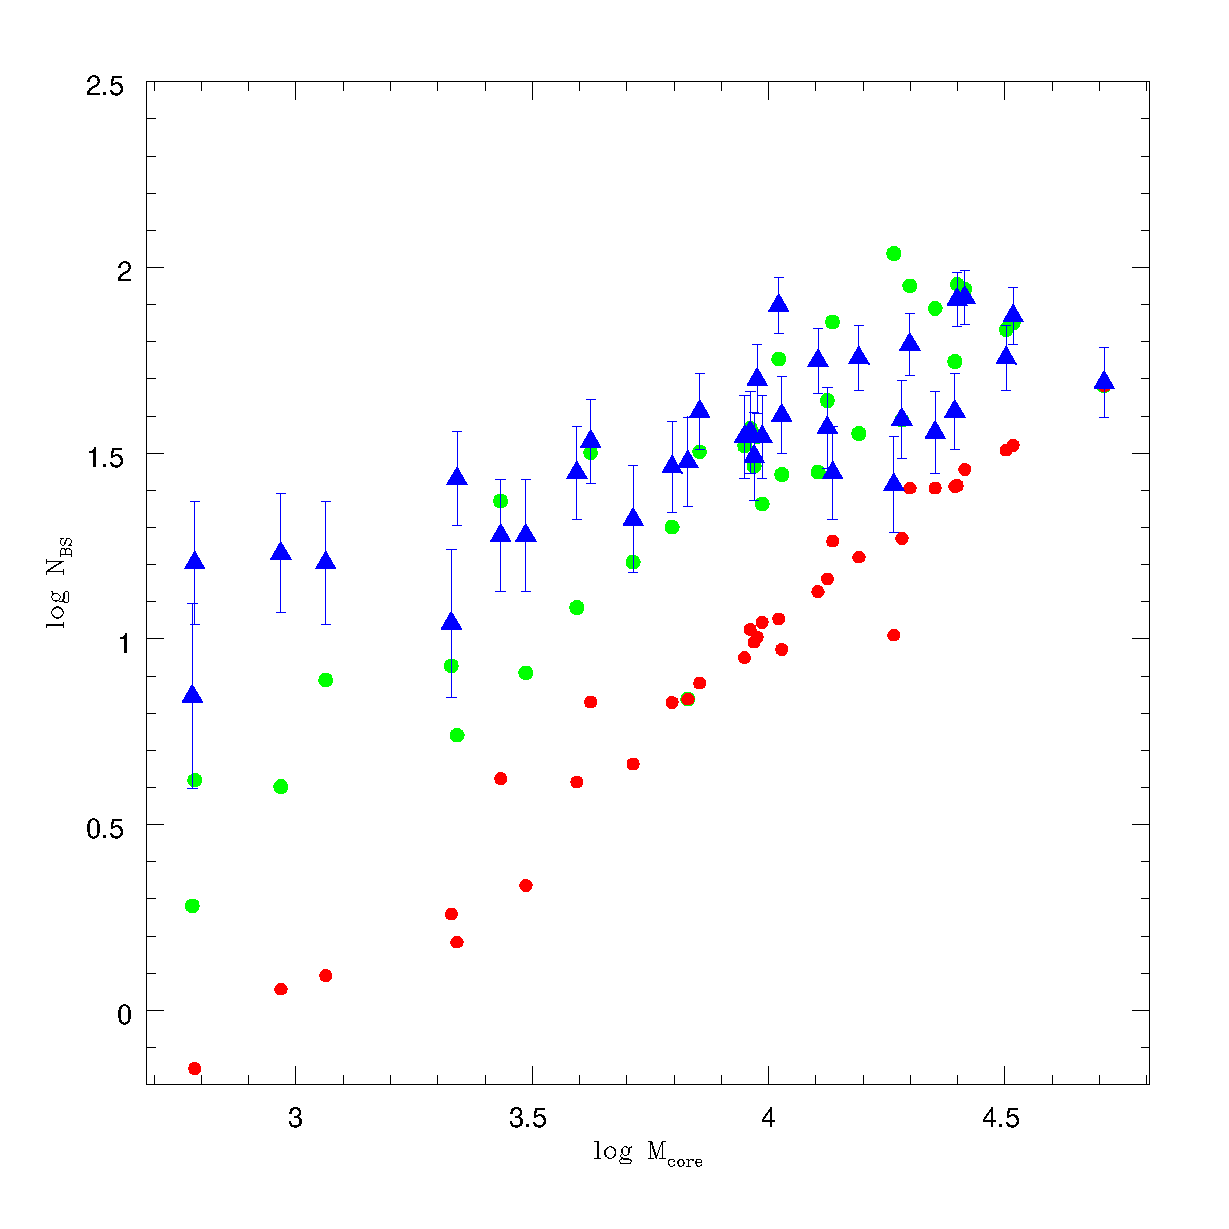
\includegraphics[scale=0.5]{Chapter-5/fig1.eps}
\caption[The predicted number of BSs plotted versus the total stellar
mass in the core for the best-fitting model parameters found for our
initial choice of assumptions]{
The predicted number of BSs plotted versus the total stellar
mass in the core for the best-fitting model parameters found for our
initial choice of assumptions.  The filled blue triangles correspond to
  the observed numbers, the 
  filled green circles to the number of BSs predicted to have formed within
  r$_{max}$, and the filled red circles to the number predicted to
  have formed in only the core.  The best-fitting model parameters
  used to calculate the predicted numbers are f$_{1+1} = 0$, f$_{1+2} = 0$,
  f$_{2+2} = 7.3 \times 10^{-3}$, and f$_{mt} = 1.7 \times 10^{-3}$.  
  Estimates for the total stellar masses in the core were obtained
  from single-mass King models, as described in \citet{leigh11a}.
  Error bars have been indicated for the observed numbers using 
  Poisson statistics.
\label{fig:model_best}}
\end{center}
\end{figure}

\subsection{Binary Fraction} \label{results-binary}

We tried changing our assumption of a constant f$_b$ for all
clusters to one for which the core binary fraction varies with the
total cluster magnitude.  First, we adopted a dependence of the
form:
\begin{equation}
\label{eqn:sollima07} 
f_b = 0.13M_V + 1.07,
\end{equation}
where M$_V$ is the total cluster V magnitude.  This 
relation comes from fitting a line of best-fit to the observations of 
\citet{sollima07}, who studied the binary fractions in a sample
of 13 low-density GCs (we calculated an average of
columns 3 and 4 in their Table 3 and used these binary fractions to
obtain Equation~\ref{eqn:sollima07}).  In order to prevent negative
binary fractions, 
we impose a minimum binary fraction of f$_b^{min} = 0.01$.  In other
words, we set f$_b =$ f$_b^{min}$ if Equation~\ref{eqn:sollima07}
gives a binary fraction less than f$_b^{min}$.  As before, we adopt an
average semi-major axis of 2 AU.  The results of this comparison are
presented in Figure~\ref{fig:model_rmax_sollima_best}.  As in
Figure~\ref{fig:model_best}, both the numbers of 
observed (blue triangles) and predicted (green circles) BSs in the
core are plotted 
versus the total stellar mass in the core.  Once again, the predicted
numbers include all BSs formed within r$_{max}$ in the last
$\tau_{BS}$ years.  The best-fitting model parameters for this
comparison suggest that both single-single collisions and binary star
evolution are significant contributors to BS formation.  Single-single
collisions contribute up to several tens of a percent of the predicted
total in several clusters.  We obtain a 
deviance in this case that is significantly larger than that obtained
for the best-fitting model parameters assuming a constant f$_b$ of
$10\%$ for all clusters.  Equation~\ref{eqn:sollima07} gives higher
binary fractions in low-mass
clusters relative to our initial assumption of a constant f$_b$.  This
increases the number of BSs formed from binary star evolution and
improves the agreement between our model predictions and the
observations in low-mass clusters.  This is consistent with the
results of \citet{sollima08}.  However, adopting
Equation~\ref{eqn:sollima07} for f$_b$ also causes our model to
under-predict the number of BSs in several high-mass clusters.

\begin{figure} [!h]
  \begin{center}
 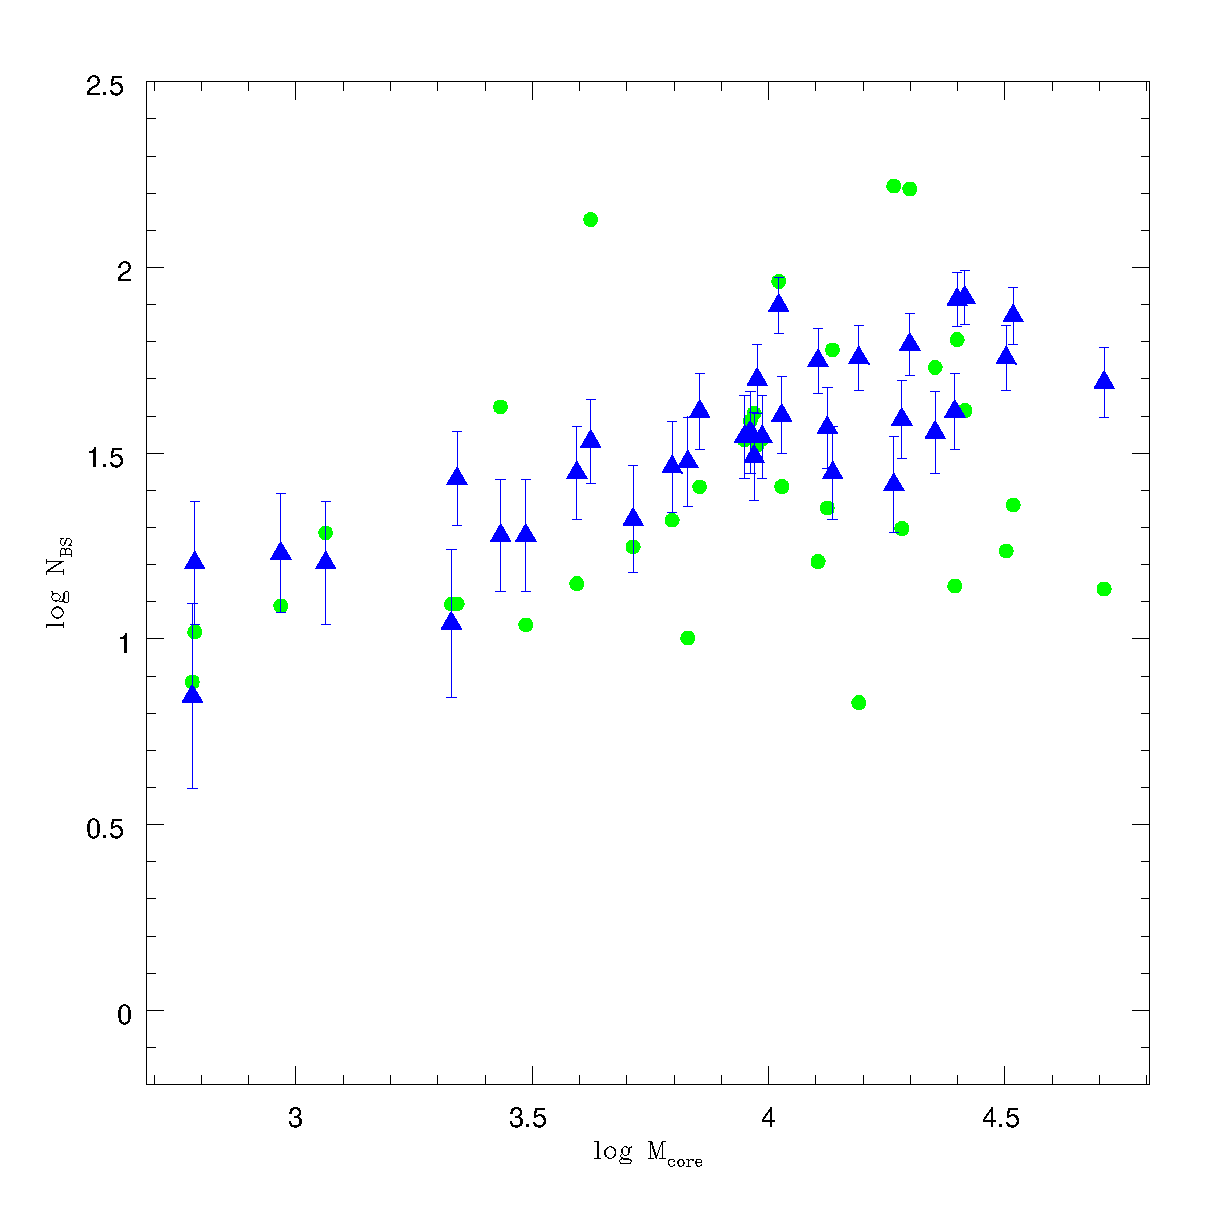
\includegraphics[scale=0.5]{Chapter-5/fig2.eps}
\caption[The predicted number of BSs plotted versus the total stellar
mass in the core for the best-fitting model parameters found using the
binary fractions of \citet{sollima07} with f$_b^{min} = 0.01$]{The
  number of BSs predicted in the cluster core using the binary
  fractions of \citet{sollima07} with f$_b^{min} = 0.01$ plotted
  against the total stellar mass contained within the core.  The
  colours used to indicate the observed and predicted numbers are the
  same as in Figure~\ref{fig:model_best}.  The predicted numbers correspond to
  the best-fitting model parameters, which are f$_{1+1} = 0.41$,
  f$_{1+2} = 0$, f$_{2+2} = 0$, and f$_{mt} = 1.5 \times 10^{-3}$.
\label{fig:model_rmax_sollima_best}}
\end{center}
\end{figure}

The best fit to the observations is found
by adopting the relation for f$_b$ provided in
Equation~\ref{eqn:sollima07} and setting f$_b^{min} = 0.1$ (however we
note that a comparably good agreement is found with a slightly lower
f$_b^{min} = 0.05$).  This
improves the agreement between our model predictions and the
observations by increasing the number of BSs formed from binary star
evolution in massive clusters.  The result is a good agreement between
our model predictions and the observations in both low- and high-mass
cores, as shown in
Figure~\ref{fig:model_best_rmax_sollima_10min_tBS15}.  In this case,
the best-fitting model parameters yield the lowest deviance of any of
the assumptions so far considered.  
These best-fitting values suggest that most BSs are formed 
from binary star evolution, with a small contribution from 2+2
collisions being needed in order to obtain the best possible match to
the observations.  Similarly to what was found for our initial
assumptions, the ideal contribution from 2+2 collisions
constitutes at most a few percent of the predicted total for most of
the clusters in our sample.  
On the other hand, if we change our imposed minimum binary fraction to
f$_b^{min} = 0.05$ we find that a non-negligible (i.e. up to a few
tens of a percent) contribution from
single-single collisions is needed in several clusters to obtain the best possible
agreement with the observations (which is very nearly as good as was
found using f$_b^{min} = 0.1$).  All of this shows that, although
binary star evolution consistently dominates BS formation in our
best-fitting models, at least some contribution from collisions
(whether it be 1+1 or 2+2 collisions, or some combination of 1+1, 1+2
and 2+2 collisions) also
consistently improves the agreement with the observations.  Moreover,
it is interesting to note that an improved agreement with the
observations could alternatively be obtained if we keep f$_b^{min} =
0.01$ but all or some of
f$_{1+1}$, f$_{1+2}$ and f$_{2+2}$ increase with increasing cluster
mass.  This would also serve to improve the agreement at the high-mass
end.  We will return to this in Section~\ref{discussion5}.

\begin{figure} [!h]
  \begin{center}
 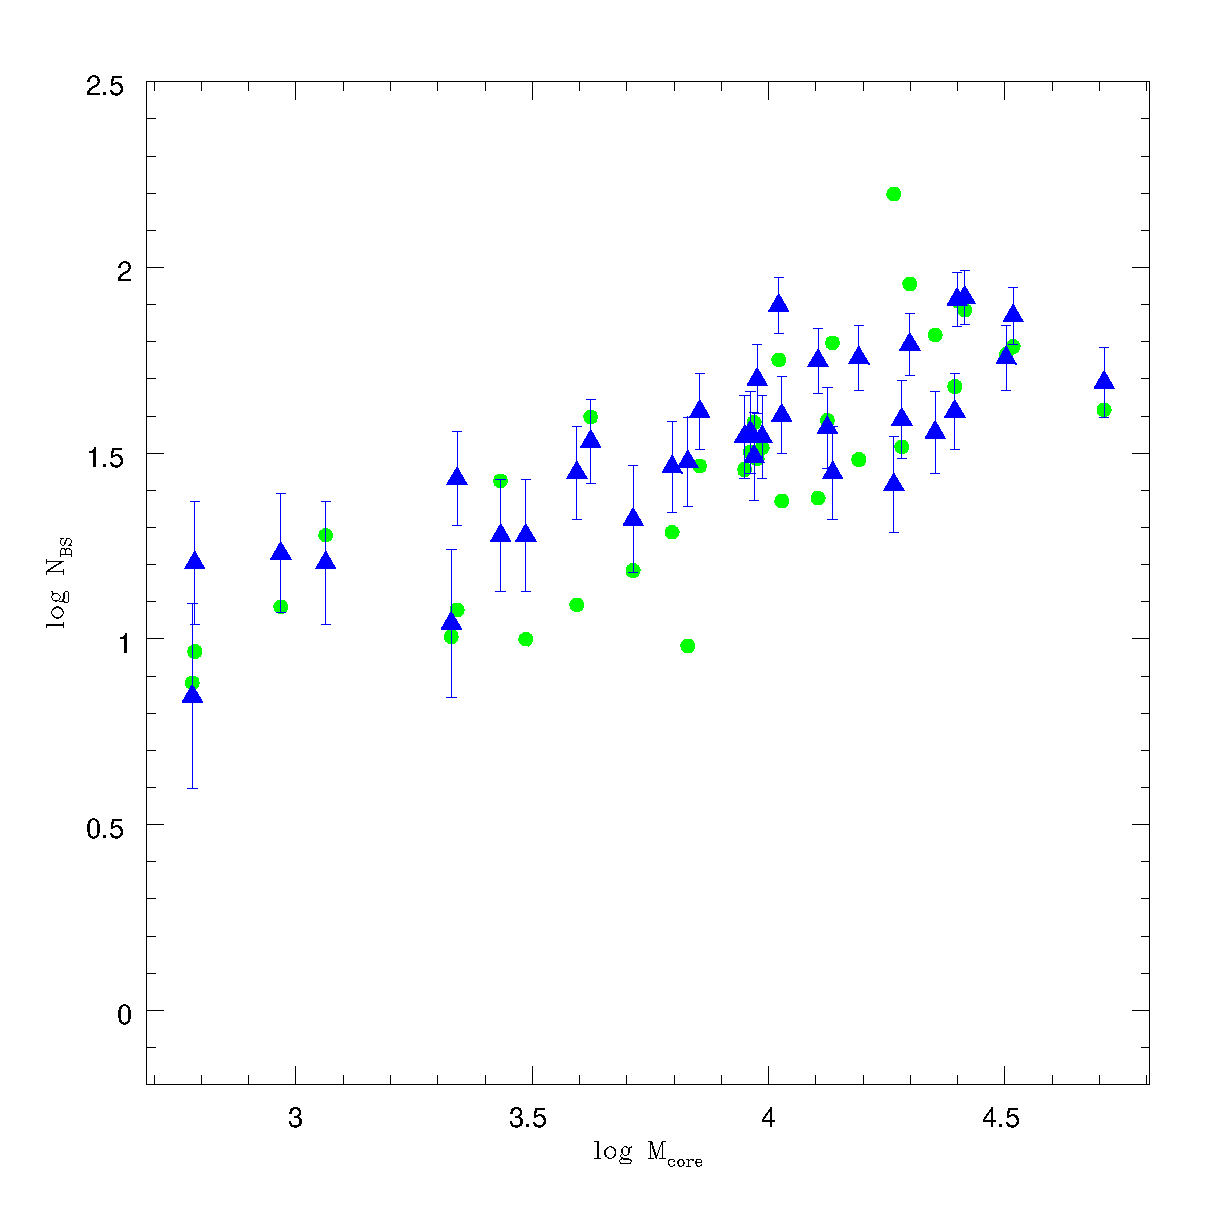
\includegraphics[scale=0.5]{Chapter-5/fig3.eps}
\caption[The predicted number of BSs plotted versus the total stellar
mass in the core for the best-fitting model parameters found using the binary
fractions of \citet{sollima07} with f$_b^{min} = 0.1$]{The number of BSs
  predicted in the cluster core using the binary fractions of
  \citet{sollima07} with f$_b^{min} = 0.1$ plotted against the total
  stellar mass contained within the core.  The
  colours used to indicate the observed and predicted numbers are the
  same as in Figure~\ref{fig:model_best}.  The predicted numbers correspond to
  the best-fitting model parameters, which are f$_{1+1} = 0$,
  f$_{1+2} = 0$, f$_{2+2} = 3.6 \times 10^{-3}$, and f$_{mt} = 1.4
  \times 10^{-3}$.
\label{fig:model_best_rmax_sollima_10min_tBS15}}
\end{center}
\end{figure}

Finally, we also tried adopting the observed dependence of f$_b$ on
M$_V$ reported in \citet{milone08}, who also found evidence for an
anti-correlation between the core binary fraction and the total
cluster mass.  Despite this change, we consistently find that our
results are the same as found when using the empirical binary fraction
relation provided in Equation~\ref{eqn:sollima07}.

\subsection{Average BS Lifetime} \label{lifetime}

We also tried changing our assumption for the average BS lifetime.  We
explored a range of plausible lifetimes based on values found
throughout the literature.  Specifically, we explored the range 0.5-5
Gyrs.  We find that at 
the low end of this range, our model fits become increasingly poor.
This is because lower values for $\tau_{BS}$ correspond to smaller
values for r$_{max}$ and decrease the term (1 -
t$_{(dyn),i}$/$\tau_{BS}$) in Equation~\ref{eqn:N-in}.  This reduces the
contribution to the total predicted 
numbers from BSs formed outside the core that fall in via dynamical 
friction.  Conversely, our model fits
improve for $\tau_{BS} > 1.5$ Gyrs since this corresponds to a larger
contribution to N$_{BS}$ from N$_{in}$.  It is important to note,
however, that this same effect can be had by increasing the 
number of BSs formed outside the core, since this would also
serve to increase N$_{in}$ in Equation~\ref{eqn:number-bss}.  This
can be accomplished by, for instance, increasing the binary fraction
outside the core (which would increase the
number of BSs formed from binary star evolution outside the core that
migrate in due to dynamical friction) relative to inside the core.
This seems unlikely, however, given that observations of low-density
globular clusters and open clusters suggest that their binary
fractions tend to drop off rapidly outside the core
\citep[e.g.][]{sollima07}.  We 
will return to this issue in Section~\ref{discussion5}.

The best possible match to the observations is
found by adopting an average BS lifetime of 5 Gyrs along with the
relation for f$_b$ provided in Equation~\ref{eqn:sollima07} with 
f$_b^{min} = 0.1$.  The predictions of our model 
are shown in Figure~\ref{fig:model_best_rmax_sollima_10min_tBS50} for
these best-fitting model parameters.  As shown, the agreement
between our model predictions and the observed numbers is excellent.
The best agreement is found by adopting an average BS lifetime of 5
Gyrs, however the agreement is comparably excellent down to 
slightly less than $\tau_{BS} \sim 3$ Gyrs.  Although increasing
$\tau_{BS}$ does contribute to improving the 
agreement between our model predictions and the observations, the
effect is minor compared to the improvement that 
can be found by changing our assumption for the binary fraction.
This is apparent upon comparing 
Figure~\ref{fig:model_best_rmax_sollima_10min_tBS50} to 
Figure~\ref{fig:model_best_rmax_sollima_10min_tBS15}.  

\begin{figure} [!h]
  \begin{center}
 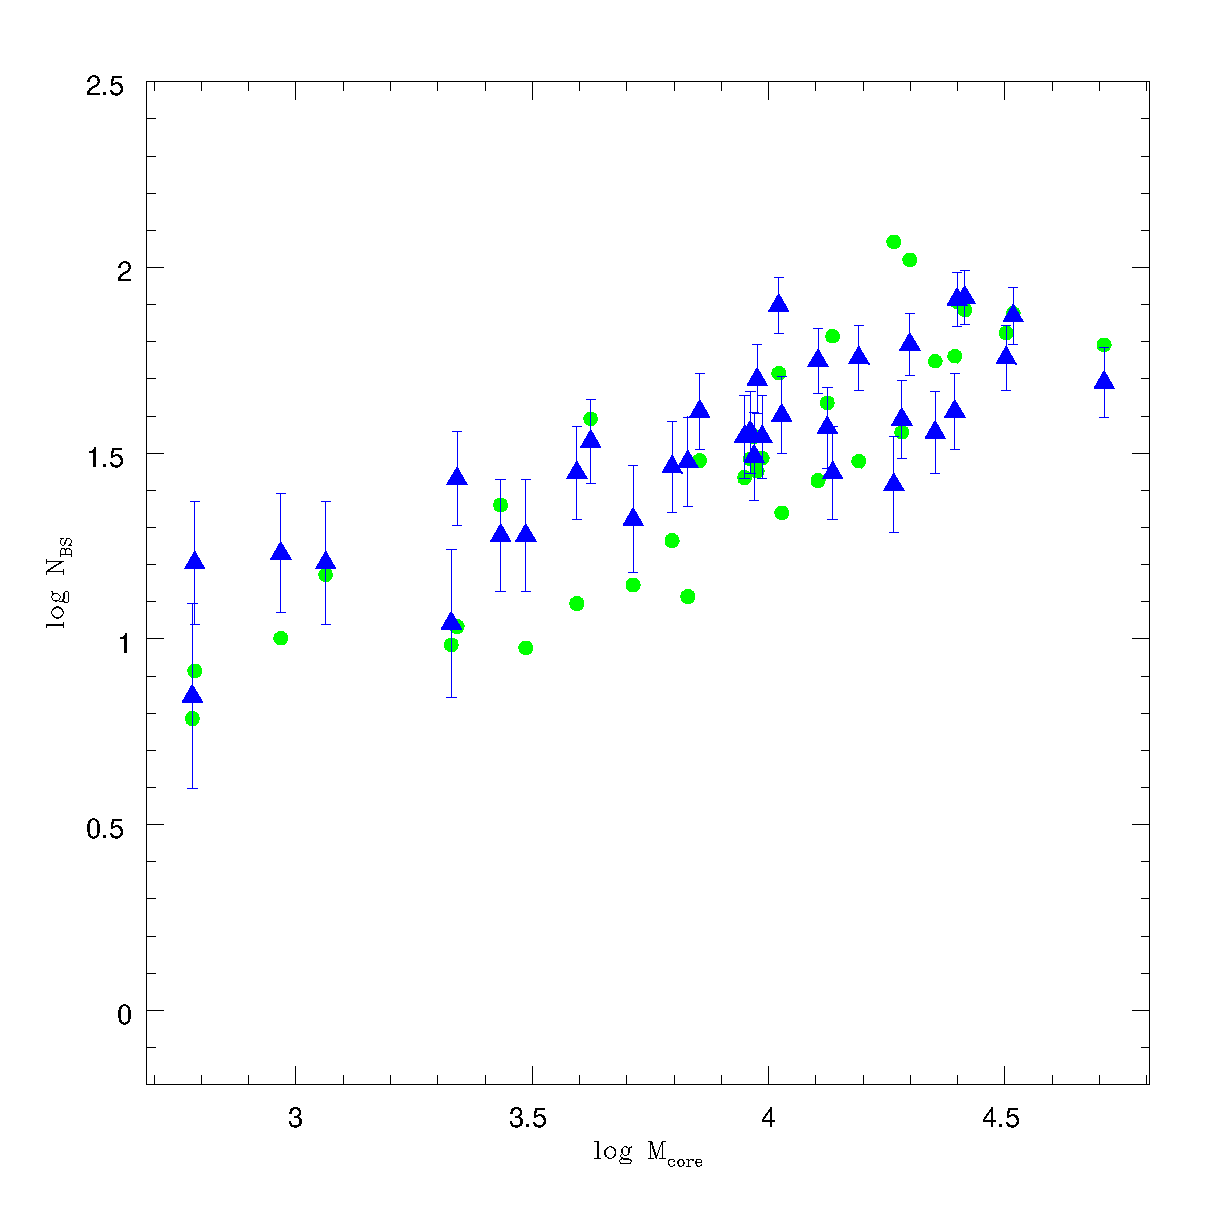
\includegraphics[scale=0.5]{Chapter-5/fig4.eps}
\caption[The predicted number of BSs plotted versus the total stellar
mass in the core for the best-fitting model parameters found using an
average BS lifetime of 5 Gyrs and the relation for the cluster binary
fraction provided in Equation~\ref{eqn:sollima07} with f$_b^{min} =
0.1$]{The predicted 
  number of BSs plotted versus the total stellar mass in the core for
  the best-fitting model parameters found using an average BS lifetime
  of 5 Gyrs and the relation for the cluster binary fraction provided
  in Equation~\ref{eqn:sollima07} with f$_b^{min} = 0.1$.  The
  colours used to indicate the observed and predicted numbers are the
  same as in Figure~\ref{fig:model_best}.  The best-fitting model parameters
  used to calculate the predicted numbers are f$_{1+1} = 0$, f$_{1+2}
  = 0$, f$_{2+2} = 1.6 \times 10^{-3}$, and f$_{mt} = 9.9 \times
  10^{-4}$.  The agreement with the observations is excellent for these
  best-fitting values.
\label{fig:model_best_rmax_sollima_10min_tBS50}}
\end{center}
\end{figure}

\subsection{Migration} \label{results-migration}

In order to explore the sensitivity of our results to our assumption
for r$_{max}$, we also tried setting N$_{in}$ equal to the total
number of BSs expected to form within 10 r$_c$ for all clusters.  For
comparison, for an average BS lifetime of $\tau_{BS} = 1.5$ Gyrs,
r$_{max}$ ranges from 2 - 15 r$_c$ for the clusters in our
sample.  Despite implementing this change, our results remained the
same.  This is because the largest contribution to the total number of
BSs comes from those BSs formed in the first few shells
immediately outside the core that migrate in due to dynamical
friction.

Several GCs have been reported to show evidence for a decrease in
their binary fractions with increasing distance from the cluster
centre \citep[e.g.][]{sollima07, davis08}.  This effect is often
significant, with binary fractions decreasing by up to a factor of a
few within only a few core radii from the cluster centre.  Based on
this, our assumption that f$_b$ is independent of the distance
from the cluster centre likely results in an over-estimate of the true
binary fraction at large cluster radii.  In order to
quantify the possible implications of this for our results, we tried
setting f$_b$ $= 0$ for all shells outside the core.  Although this
assumption is certainly an under-estimate for the true binary fraction
outside the core, our results remain the same (albeit the agreement
with the observations is considerably worse than for most of our previous
model assumptions).  Once again, the
best-fitting model parameters suggest that most BSs are formed from
binary star evolution, with a non-negligible (i.e. up to a few tens of
a percent in some clusters) contribution from
binary-binary collisions.  Our results indicate that, if the
binary fraction is negligible outside the core, then the contribution
from BSs that migrate into the core due to dynamical friction is also
negligible.  This is because the time between 1+1 collisions increases
rapidly outside the core, and every other BS formation mechanism requires
binary stars to operate.  %We will return to this issue in
%Section~\ref{discussion}.

We also explored the effects of assuming a non-zero value for
N$_{out}$ in Equation~\ref{eqn:number-bss} by imparting a constant
kick velocity to all
BSs at birth.  Using conservation of energy, we calculated the
cluster radius to which BSs should be kicked upon formation, and used
the time-scale for dynamical friction at the kick radius to calculate
the fraction of BSs expected to migrate back into the core within
a time $\tau_{BS}$.  Regardless of our assumption for the kick
velocity, this did not improve the deviance for any of our
best-fitting model parameters.

\subsection{Average Binary Semi-Major Axis} \label{avg-a}

We investigated the dependence of our results on our assumption for
the average binary semi-major axis.  However, this had a very small
effect on our results.  This is because only N$_{1+2}$ and N$_{2+2}$
depend on the average semi-major axis, and neither of these terms
dominated BS production regardless of our model
assumptions.  Only f$_{2+2}$ is
non-zero for our best-fitting models however, as before, it consistently
suggests that far fewer BSs should be formed from 2+2 collisions than from
binary star evolution. 

\section{Summary \& Discussion} \label{discussion5}

In this chapter, we have presented an analytic model to investigate BS
formation in globular clusters.  Our model predicts the number of BSs
in the cluster core at the current cluster age by estimating the
number that should have either formed 
there from stellar collisions and binary star evolution, or migrated
in via dynamical friction after forming outside the core.  We have
compared the results of our model predictions for a variety of input
parameters to observed BS numbers in 35 GCs taken from the catalogue of
\citet{leigh11a}.   

What has our model told us about BS formation in dense cluster
environments?  
The agreement between the predictions of our model and the
observations is excellent if we assume that:

\begin{itemize}

\item Binary star evolution dominates BS formation, however at least
  some contribution from 2+2 collisions (most of which
  occur in the core) must also be included in the total predicted
  numbers.  Although it is clear that including a contribution from
  dynamical encounters gives the best possible match to the
  observations, it is not clear how exactly this is accomplished in
  real star clusters.  Does the cluster dynamics increase
  BS numbers via direct collisions?  Or do dynamical interactions
  somehow modify primordial binaries to initiate more mass-transfer
  events?  We will return to this point below.

\item The binary fraction in the core is inversely
  correlated with the total cluster luminosity, similar to the
  empirical relations found by \citet{sollima07} and \citet{milone08}.
  We also require a minimum core binary fraction of $5-10\%$.  The
  inverse dependence of f$_b$ on the total cluster mass
  contributes to a better agreement with the observations at the
  low-mass end of the distribution of cluster masses, whereas 
  the imposed condition that f$_b^{min} = 0.05 - 0.1$ contributes to
  improving the agreement at the high-mass end.

\item BSs formed outside the core that migrate in by the
  current cluster age contribute to the total predicted numbers.

\item The average BS lifetime is roughly a few ($\sim$ 3-5) Gyrs, since this
  increases the fraction of BSs formed outside the core that will have
  sufficient time to migrate in due to dynamical friction.

\end{itemize}

Our model can only provide a
reasonable fit to the observations for all cluster masses if we assume
that the cluster binary fraction is inversely proportional to the total
cluster mass.  It is interesting to consider the possibility that such
an inverse proportionality could 
arise as a result of the fact that the rate of two-body relaxation is
also inversely proportional to the cluster mass \citep{spitzer87}.
Consequently, since binaries tend to be the most massive objects in
GCs, they should quickly migrate into the core in low-mass clusters,
contributing to an increase in the core binary fraction over
time \citep{fregeau09}.  This process should operate on a considerably
longer time-scale in very massive GCs since the time-scale for
two-body relaxation is very long.  Mass segregation could then 
contribute to the observed sub-linear dependence of BS numbers
on the core masses by acting to preferentially migrate the binary star
progenitors of BSs into the cores of low-mass clusters.  This is one
example of how a direct link could arise between the observed
properties of BS 
populations and the dynamical histories of their host clusters.
Although this scenario is interesting to consider, we 
cannot rule out the possibility that an anti-correlation between the
core binary fraction and the total cluster mass could be a primordial
property characteristic of GCs at birth.

When interpreting our results, it is important to bear in mind that
binary star evolution and dynamical interactions involving binaries
may not always contribute to BS formation independently.  For example,
dynamics could play an important role in changing the distribution of
binary orbital parameters so that mass-transfer occurs more commonly
in some clusters.  
One way to perhaps compensate for this effect would be to include 
a factor of $1/a$ (where $a$ is the average binary semi-major axis) in
Equation~\ref{eqn:N-bin}.  This would serve to account for the fact
that we might naively expect clusters populated by more close binaries
to be 
more likely to have a larger fraction of their binary populations
undergo mass-transfer.  This does not, however, guarantee that more
BSs will form since our poor understanding of binary star evolution
prevents us from being able to predict the outcomes of these
mass-transfer events, and whether or not they will form BSs.
Moreover, little is known about the distribution of orbital
parameters characteristic of the binary populations in globular
clusters, and how they are typically modified by the cluster
dynamics.  For 
these reasons, the interpretation of our results must be done with
care in order to ensure that reliable conclusions can be drawn.
%Although it is clear from our results that
%including a contribution from dynamical encounters consistently
%improves the match to the observations from what we obtain by
%considering binary star evolution alone, it is not clear how exactly
%this occurs in real star clusters.  Does the cluster dynamics increase
%BS numbers directly via stellar collisions?  Or do dynamical interactions
%somehow modify primordial binaries to initiate more mass-transfer
%events?

In general, our results suggest that binary stars play a crucial role
in BS formation in dense GCs.  
In order to obtain the best possible agreement with the observations,
an enhancement in BS formation from dynamical encounters is required
in at least some clusters relative to what is expected by assuming a
simple population of binaries evolving in isolation.  It is not clear
from our results, however, how exactly this occurs in real star
clusters.  Dynamics could enhance BS
formation directly by causing stellar collisions, or this could
also occur indirectly if the cluster dynamics somehow induces episodes of
mass-transfer by reducing the orbital 
separations of binaries.  But in which clusters is
BS formation the most strongly influenced by the cluster dynamics?
Unfortunately, no clear trends have emerged from our analysis that
provide a straight-forward answer to this question.  However, our
results are consistent with dynamical interactions 
playing a more significant role in more massive clusters (although
this does not imply that the cluster dynamics does not also contribute
in low-mass clusters).  This could 
be due to the fact that more massive clusters also tend to have higher
central densities \citep[e.g.][]{djorgovski94}, and therefore
higher collision rates.  This picture is, broadly speaking, roughly
consistent with 
the results of \citet{davies04}.  These authors considered the observed
dependence (or lack thereof) of BS numbers on the total cluster masses
presented in \citet{piotto04}, and suggested that primordial binary
evolution and stellar collisions dominate BS production in low- and
high-mass clusters, respectively.

Our model neglects the dynamical evolution of GCs and the resulting
changes to their global properties, including the central density,
velocity dispersion, core radius and binary fraction.  As a young
cluster evolves, dynamical processes like mass segregation and
stellar evaporation tend to result in a smaller, denser core.  Within
a matter of a few half-mass relaxation times, a gravothermal
instability has set in and the collapse ensues on a time-scale
determined by the rate of heat flow out of the core
\citep[e.g.][]{spitzer87}.  We are focussing 
on the last $\tau_{BS}$ years of cluster 
evolution, a sufficiently late period in the lives of most GCs
that gravothermal collapse will have long since taken over as the
primary driving force affecting the stellar concentration in the
core.  Most of the GCs in our sample should currently be in a phase
of core contraction \citep{fregeau09, gieles11}, and their central
densities and core radii should have been steadily
decreasing over the last $\tau_{BS}$ years.  Therefore, by using
the currently observed central cluster parameters and assuming that
they remained constant over the last
$\tau_{BS}$ years, we have effectively calculated upper limits for
the encounter rates.  This could suggest that we have over-estimated
the importance of dynamical interactions for BS formation.  On the
other hand, some theoretical
models of GC evolution suggest that the hard binary fraction in the
core of a dense stellar system will generally increase
with time \citep[e.g.][]{hurley05, fregeau09}.  This can be understood as an
imbalance between the migration of
binaries into the core via mass segregation and the destruction of
binaries in the core via both dynamical encounters and their internal
evolution.  This could suggest that our estimate for the number of BSs
formed from binary star evolution should also be taken as an upper
limit.  The key point is that GC evolution can act to
increase the number of BSs in the cluster core via several different
channels.  The effects we have discussed should typically be small,
however, since 
$\tau_{BS}$ is much shorter than the cluster age \citep{deangeli05}
and any changes to global cluster properties that occur during this
time will often be small.

Our model adopts the same values for all free parameters in all
clusters.  In particular, this is the case for several global cluster
properties, including the average stellar mass, the average BS 
mass, the average BS lifetime, and the average 
binary semi-major axis.  With the exception of the average stellar
mass, there is no conclusive observational or theoretical
evidence to indicate that these parameters should differ from
cluster-to-cluster, although we cannot rule out this possibility.  
For instance, the distribution of binary orbital parameters could
depend on cluster properties 
like the total mass, density or velocity dispersion
\citep[e.g.][]{sigurdsson93}.  In particular, the central velocity
dispersion should be higher in more massive GCs
\citep[e.g.][]{djorgovski94}, which should correspond to a smaller
binary orbital separation for the hard-soft boundary.  
This could contribute to massive GCs tending to have smaller average
binary orbital separations since soft binaries should not survive
for long in the dense cores of GCs \citep[e.g.][]{heggie03}.  In turn,
this could 
%facilitate an
%increased occurrence of mass-transfer events in massive GCs, or of 
%mergers during 1+2 and 2+2 encounters.  This last point follows from
affect the occurrence of mass-transfer events, or of 
mergers during 1+2 and 2+2 encounters.  This last point follows from
the fact that numerical scattering experiments have shown that the 
probability of mergers occurring during 1+2 and 2+2 interactions
increases with decreasing binary orbital separation
\citep[e.g.][]{fregeau04}.  Both the average stellar mass and the
average BS mass (and hence lifetime) could also depend on the total 
cluster mass, as discussed in \citet{leigh09} and \citet{leigh11a}.

We have also neglected to consider the importance of triples for BS
formation throughout our analysis \citep[e.g.][]{perets09} since we
are unaware of any 
observations of triples in GCs in the literature.  Interestingly,
however, our results for binary star evolution can be generalized to
include the internal evolution of triples since they should have the
same functional dependence on the core mass (i.e. N$_{te} \propto
f_tM_{core}$, where N$_{te}$ is the number of BSs formed from triple
star evolution and f$_{t}$ is the fraction of objects that are
triples). 

Finally, our model 
assumes that several parameters remain constant as a function of
the distance from the cluster centre, including the binary fraction
and the average 
semi-major axis.  However, observations of GCs suggest that their
binary fractions could fall off rapidly outside the core
\citep[e.g.][]{sollima07, davis08}.  Our results suggest that, if the
binary fraction is negligible outside the core, then the contribution
from BSs that migrate into the core due to dynamical friction is also
negligible.  This is because the time between 1+1 collisions increases
rapidly outside the core, and every other BS formation mechanism requires
binary stars to operate.  On the other hand, the presently observed
binary fraction outside the core could be low as a result of binaries
having previously migrated into the core due to dynamical friction
\citep[e.g.][]{fregeau09}.  If these are the binary star progenitors
of the BSs currently populating the core, then dynamical friction
remains an important effect in determining the number of BSs
currently populating the core. 

Despite all of these 
simplifying assumptions, we have shown that our model can reproduce the 
observations with remarkable accuracy.  Notwithstanding, the effects
we have discussed 
could be contributing to cluster-to-cluster differences in the
observed BS numbers.  Our model provides a well-suited resource for
addressing the role played by these effects, however future
observations will be needed in order to obtain the desired constraints
(e.g. binary fractions, distributions of binary orbital parameters, etc.).   

\section*{Acknowledgments}

We would like to thank Ata Sarajedini, Aaron Dotter and Roger Cohen
for providing the observations to which we compared our model
predictions, as well as for providing a great deal of guidance in 
analyzing the data.  We would also like to thank Evert Glebbeek, Bob Mathieu
and Aaron Geller for useful discussions.  This research has been
supported by NSERC and OGS. 

%\chapterbib

\begin{thebibliography}{99}

\bibitem[\protect\citeauthoryear{Anderson et al.}{2008}]{anderson08}
  Anderson J.,  Sarajedini A., Bedin L. R., King I. R., Piotto G.,
  Reid I. N., Siegel M., Majewski S. R., Paust N. E. Q., Aparicio A.,
  Milone A. P., Chaboyer B., Rosenberg A. 2008, AJ, 135, 2055
\bibitem[\protect\citeauthoryear{Andrievsky et al.}{2000}]{andrievsky00} Andrievsky S. M.,
  Schonberner D., Drilling J. S. 2000, A\&A, 356, 517
\bibitem[\protect\citeauthoryear{Bacon et al.}{1996}]{bacon96} Bacon
  D., Sigurdsson S., Davies M. B. 1996, MNRAS, 281, 830
\bibitem[\protect\citeauthoryear{Binney \& Tremaine}{1987}]{binney87} Binney J., Tremaine S. 1987,
  Galactic Dynamics (Princeton: Princeton University Press)
\bibitem[\protect\citeauthoryear{Cool et al.}{2002}]{cool02} Cool A. M., Bolton
  A. S. 2002, in ASP Conference Series 263, Stellar Collisions,
  Mergers and their Consequences, ed. M. M. Shara (San Francisco:
  ASP), 163
\bibitem[\protect\citeauthoryear{Davies, Piotto \& De
    Angeli}{2004}]{davies04} Davies M. B., Piotto G., De Angeli
  F. 2004, MNRAS, 348, 129
\bibitem[\protect\citeauthoryear{Davis et al.}{2008}]{davis08}
  Davis D. S., Richer H. B., Anderson J., Brewer J., Hurley J.,
  Kalirai J. S., Rich R. M., Stetson P. B. 2008, AJ, 135, 2155
\bibitem[\protect\citeauthoryear{De Angeli et al.}{2005}]{deangeli05}
  De Angeli F., Piotto G., Cassisi S., Busso G., Recio-Blanco A.,
  Salaris M., Aparicio A., Rosenberg A. 2005, AJ, 130, 116
\bibitem[\protect\citeauthoryear{Dervisoglu, Tout \& Ibanoglu}{2010}]{dervisoglu10} Dervisoglu A., Tout C. A., Ibanoglu
  C. 2010, MNRAS, 406, 1071
\bibitem[\protect\citeauthoryear{Djorgovski \&
    Meylan}{1994}]{djorgovski94} Djorgovski S., Meylan G. 1994, ApJ, 108, 1292
\bibitem[\protect\citeauthoryear{Ferraro et al.}{1997}]{ferraro97}
  Ferraro F. R., Paltrinieri B., Fusi Pecci F., Cacciari C., Dorman
  B., Rood R. T., Buonanno R., Corsi C. E., Burgarella D., Laget
  M. 1997, A\&A, 324, 915
\bibitem[\protect\citeauthoryear{Ferraro et al.}{1999}]{ferraro99}
  Ferraro F. R., Paltrinieri B., Rood R. T., Dorman B. 1999, ApJ, 522,
  983
\bibitem[\protect\citeauthoryear{Ferraro et al.}{2004}]{ferraro04}
  Ferraro F. R., Beccari G., Rood, R. T., Bellazzini M., Sills A.,
  Sabbi E. 2004, ApJ, 603, 127
\bibitem[\protect\citeauthoryear{Fregeau et al.}{2004}]{fregeau04} Fregeau J. M., Cheung P.,
  Portegies Zwart S. F., Rasio F. A. 2004, MNRAS, 352, 1
\bibitem[\protect\citeauthoryear{Fregeau, Ivanova \& Rasio}{2009}]{fregeau09} Fregeau J. M., Ivanova N.,
  Rasio F. A. 2009, ApJ, 707, 1533
\bibitem[\protect\citeauthoryear{Geller at al.}{2009}]{geller09}
  Geller A. M., Mathieu R. D., Harris H. C., McClure R. D., 2009,
  AJ, 137, 3743
\bibitem[\protect\citeauthoryear{Gieles, Heggie \& Zhao}{2011}]{gieles11}
  Gieles M., Heggie D., Zhao H. 2011, MNRAS, accepted
\bibitem[\protect\citeauthoryear{Glebbeek \& Pols}{2008}]{glebbeek08} Glebbeek E., Pols
  O. R. 2008, A\&A, 488, 1017
\bibitem[\protect\citeauthoryear{Guhathakurta et al.}{1998}]{guhathakurta98} Guhathakurta 
  P., Webster Z. T., Yanny B., Schneider D. P., Bahcall J. N. 1998,
  AJ, 116, 1757
\bibitem[\protect\citeauthoryear{Harris et al.}{1996}]{harris96} Harris W. E. 1996, AJ, 112,
  1487; 2010 update
\bibitem[\protect\citeauthoryear{Heggie \& Hut}{2003}]{heggie03}
  Heggie D. C., Hut P. 2003, The Gravitational Million-Body Problem:
  A Multidisciplinary Approach to Sar Cluster Dynamics (Cambridge:
  Cambridge University Press)
\bibitem[\protect\citeauthoryear{Hurley et al.}{2005}]{hurley05}
  Hurley J. R., Pols O. R., Aarseth S. J., Tout C. A. 2005, MNRAS,
  363, 293
\bibitem[\protect\citeauthoryear{Hurley, Aarseth \&
    Shara}{2007}]{hurley07} Hurley J. R., Aarseth S. J., Shara M. M. 2007, ApJ, 665, 707
\bibitem[\protect\citeauthoryear{Hut \& Bahcall}{1983}]{hut83} Hut P., Bahcall J. N. 1983, ApJ,
  268, 319 
\bibitem[\protect\citeauthoryear{Iben}{1991}]{iben91} Iben I. Jr. 1991, ApJS, 76, 55
\bibitem[\protect\citeauthoryear{Ivanova et al.}{2005}]{ivanova05}
  Ivanova N., Belczynski K., Fregeau J. M., Rasio F. A. 2005, MNRAS, 358, 572
\bibitem[\protect\citeauthoryear{King, Sosin \& Cool}{1995}]{king95}
  King I. R., Sosin C., Cool A. M. 1995, ApJ, 452, L33
\bibitem[\protect\citeauthoryear{Knigge, Leigh \& Sills}{2009}]{knigge09} Knigge C., Leigh
  N., Sills A. 2009, Nature, 457, 288
\bibitem[\protect\citeauthoryear{Latham}{2005}]{latham05} Latham
  D. W., 2005, Highlights of Astronomy, 14, 444
\bibitem[\protect\citeauthoryear{Lanzoni et al.}{2007}]{lanzoni07}
  Lanzoni B., Dalessandro E., Perina S., Ferraro F. R., Rood R. T.,
  Sollima A. 2007, ApJ, 670, 1065
\bibitem[\protect\citeauthoryear{Leigh, Sills \& Knigge}{2007}]{leigh07} Leigh
  N. W., Sills A., Knigge C. 2007, ApJ, 661, 210
\bibitem[\protect\citeauthoryear{Leigh, Sills \& Knigge}{2008}]{leigh08} Leigh
  N. W., Sills A., Knigge C. 2008, ApJ, 678, 564
\bibitem[\protect\citeauthoryear{Leigh, Sills \& Knigge}{2009}]{leigh09} Leigh
  N. W., Sills A., Knigge C. 2009, MNRAS, 399, L179
\bibitem[\protect\citeauthoryear{Leigh \& Sills}{2011}]{leigh11b} Leigh
  N. W., Sills A. 2011, MNRAS, 410, 2370
\bibitem[\protect\citeauthoryear{Leigh, Sills \& Knigge}{2011}]{leigh11a} Leigh
  N. W., Sills A., Knigge C. 2011, MNRAS, accepted
\bibitem[\protect\citeauthoryear{Leonard}{1989}]{leonard89} Leonard
  P. J. T. 1989, AJ, 98, 217
\bibitem[\protect\citeauthoryear{Leonard \& Linnell}{1992}]{leonard92}
  Leonard P. J. T., Linnell A. P. 1992, AJ, 103, 1928
\bibitem[\protect\citeauthoryear{Leonard \& Livio}{1995}]{leonard95} Leonard P. J. T., Livio M. 1995,
  ApJ, 447, L121
\bibitem[\protect\citeauthoryear{Li \& Zhang}{2006}]{li06} Li L.,
  Zhang F. 2006, MNRAS, 369, 2001
\bibitem[\protect\citeauthoryear{Lombardi et al.}{2002}]{lombardi02}
  Lombardi J. C., Warren J. S., Rasio F.A., Sills A., Warren A. R. 2002, ApJ, 568, 939
\bibitem[\protect\citeauthoryear{Mapelli et al.}{2004}]{mapelli04}
  Mapelli M., Sigurdsson S., Colpi M., Ferraro F. R., Possenti A., Rood R. T., Sills A., Beccari G. 2004, ApJ, 605, L29
\bibitem[\protect\citeauthoryear{Mapelli et al.}{2006}]{mapelli06}
  Mapelli M., Sigurdsson S., Ferraro F. R., Colpi M., Possenti A., Lanzoni B. 2006,
  MNRAS, 373, 361
\bibitem[\protect\citeauthoryear{Mathieu \& Geller}{2009}]{mathieu09}
  Mathieu R. D., Geller A. R. 2009, Nature, 462, 1032
\bibitem[\protect\citeauthoryear{McCrea}{1964}]{mccrea64} McCrea
  W. H. 1964, MNRAS, 128, 147
\bibitem[\protect\citeauthoryear{McLaughlin \& van den
    Marel}{2005}]{mclaughlin05} McLaughlin D. E., van der Marel
  R. P. 2005, ApJS, 161, 304 
\bibitem[\protect\citeauthoryear{McMillan}{1986}]{mcmillan86} McMillan S. L. W. 1986, ApJ,
  306, 552
\bibitem[\protect\citeauthoryear{Milone et al.}{2008}]{milone08}
  Milone A. P., Piotto G., Bedin L. R., Sarajedini A. 2008, MmSAI, 79,
  623
\bibitem[\protect\citeauthoryear{Piotto et al.}{2004}]{piotto04}
  Piotto G., De Angeli F., King I. R., Djorgovski S. G., Bono G.,
  Cassisi S., Meylan G., Recio-Blanco A., Rich R. M., Davies M. B. 2004,
  ApJ, 604, L109
\bibitem[\protect\citeauthoryear{Perets \& Fabrycky}{2009}]{perets09}
  Perets H. B., Fabrycky D. C. 2009, ApJ, 697, 1048
\bibitem[\protect\citeauthoryear{Rubenstein \&
    Bailyn}{1997}]{rubenstein97} Rubenstein E. P., Bailyn C. D. 1997,
  ApJ, 474, 701
\bibitem[\protect\citeauthoryear{Sandage}{1953}]{sandage53}
  Sandage A. R. 1953, AJ, 58, 61
\bibitem[\protect\citeauthoryear{Sandquist, Bolte \&
    Hernquist}{1997}]{sandquist97} Sandquist E. L., Bolte M., Hernquist L. 1997, ApJ, 477, 335
\bibitem[\protect\citeauthoryear{Sarajedini et al.}{2007}]{sarajedini07}
  Sarajedini A., Bedin L. R., Chaboyer B., Dotter  A., Siegel M.,
  Anderson J., Aparicio A., King I., Majewski S., Marin-Franch A.,
  Piotto G., Reid  I. N., Rosenberg A., Steven M. 2007, AJ, 133, 1658
\bibitem[\protect\citeauthoryear{Sigurdsson \&
    Phinney}{1993}]{sigurdsson93} Sigurdsson S., Phinney E. S. 1993, ApJ, 415, 631
\bibitem[\protect\citeauthoryear{Saviane et al.}{1998}]{saviane98}
  Saviane I., Piotto G., Fagotto F., Zaggia S., Capaccioli M.,
  Aparicio A. 1998, A\&A, 333, 479
\bibitem[\protect\citeauthoryear{Shara et al.}{1995}]{shara95} Shara
  M. M., Drissen L., Bergeron L. E.,  Paresce F. 1995, ApJ, 441, 617
\bibitem[\protect\citeauthoryear{Shara, Saffer \&
    Livio}{1997}]{shara97} Shara M. M., Saffer R. A., Livio M. 1997,
  ApJ, 489, L59
\bibitem[\protect\citeauthoryear{Sills \& Bailyn}{1999}]{sills99} Sills A., Bailyn C. D. 1999,
  ApJ, 513, 428 
\bibitem[\protect\citeauthoryear{Sills et al.}{2001}]{sills01} Sills A. R., Faber J. A.,
  Lombardi J. C., Rasio F. A., Waren A. R. 2001, ApJ, 548, 323
\bibitem[\protect\citeauthoryear{Sollima et al.}{2007}]{sollima07}
  Sollima A., Beccari G., Ferraro F. R., Fusi Pecci F., Sarajedini
  A. 2008, MNRAS, 380, 781
\bibitem[\protect\citeauthoryear{Sollima et al.}{2008}]{sollima08}
MN-11-0613-MJ  Sollima A., Beccari G., Ferraro F. R., Fusi Pecci F., Sarajedini
  A. 2007, A\&A, 481, 701 
\bibitem[\protect\citeauthoryear{Spitzer}{1969}]{spitzer69} Spitzer
  L. Jr. 1969, ApJ, 168, L139
\bibitem[\protect\citeauthoryear{Spitzer}{1987}]{spitzer87} Spitzer L. 1987, Dynamical
  Evolution of Globular Clusters (Princeton: Princeton University
  Press)
\bibitem[\protect\citeauthoryear{Stryker}{1993}]{stryker93} Stryker L. L. 1993,
  PASP, 105, 1081
\bibitem[\protect\citeauthoryear{van den Berg et al.}{2001}]{vandenberg01} van den Berg M.,
  Orosz J., Verbunt F., Stassun K. 2001, A\&A, 375, 375
\bibitem[\protect\citeauthoryear{Verbunt, Pooley \&
    Bassa}{2008}]{verbunt08} Verbunt F., Pooley D., Bassa C. 2008, IAU
  Symposium 246, 301
\bibitem[\protect\citeauthoryear{Webbink}{1985}]{webbink85} Webbink R. F. 1985, in Dynamics of
  Star Clusters, IAU Symp. 113, ed. J. Goodman \& P. Hut (Dordrecht: 
  Reidel), 541

\end{thebibliography}

%\bsp

%\label{lastpage}

\pagestyle{fancy}
\headheight 20pt
\lhead{Ph.D. Thesis --- N. Leigh }
\rhead{McMaster - Physics \& Astronomy}
\chead{}
\lfoot{}
\cfoot{\thepage}
\rfoot{}
\renewcommand{\headrulewidth}{0.1pt}
\renewcommand{\footrulewidth}{0.1pt}

\chapter{A New Quantitative Method for Comparing the Stellar Mass
  Functions in a Large Sample of Star Clusters:  Evidence for a
  Universal Initial Mass Function in Massive Star Clusters in the
  Early Universe} \label{chapter6}
%Quantifying the Universality of the Initial Stellar Mass
%  Function}
%%%\author[Nathan Leigh, Alison Sills and Christian Knigge]{Nathan Leigh$^{1}$,
%%%  Alison Sills$^{1}$, Christian Knigge$^{2}$\thanks{E-mail:
%%%    leighn@mcmaster.ca (NL);
%%%    asills@mcmaster.ca (AS); christian@astro.soton.ac.uk (CK)} \\
%%%$^{1}$Department of Physics and Astronomy, McMaster University,
%%%1280 Main St. W., Hamilton, ON, L8S 4M1, Canada \\
%%%$^{2}$School of Physics and Astronomy, University of Southampton,
%%%Highfield, Southampton, SO17 1BJ, United Kingdom}
\thispagestyle{fancy}

%\begin{document}

%%%\pagerange{\pageref{firstpage}--\pageref{lastpage}} \pubyear{2010}

%%%\maketitle

%%%\label{firstpage}

%%%\begin{abstract}

%%%\end{abstract}
%
%%%\begin{keywords}
%ADD MORE KEY WORDS.
%%%globular clusters: general -- stellar dynamics -- stars: statistics -- catalogues.
%%%\end{keywords}

\section{Introduction} \label{intro6}
It is now known that most, if not all, of the stars in our Galaxy were
born in star clusters \citep[e.g.][]{lada95, lada03, mckee07}.  And yet, 
there remain several key details of the star formation process that are still
not understood.  Part of the 
problem lies in the fact that populations of young stars are typically
hidden by a dense veil of optically-thick gas and dust.  This
prevents the escape of most of the light produced by infant stars, and
often renders these regions difficult to observe \citep[e.g.][]{grenier05,
  lada07}.  Most of 
these clusters are sparsely populated and are of relatively low mass (M
$\lesssim$ 10$^4$ M$_{\odot}$) \citep[e.g.][]{lada85}.  They are also
very young since these clusters are unlikely to survive for more than
1 Gyr \citep[e.g.][]{portegieszwart10}.    
At the other end of the mass spectrum, most massive star clusters (M
$\gtrsim$ 10$^4$ M$_{\odot}$) in our Galaxy tend to be at least a few
Gyrs old, and 
in many cases are nearly as old as the Universe itself
\citep[e.g.][]{harris96, deangeli05}.  %As a point of comparison, a
%cluster with an initial 
%number of stars $N \sim 10^5$ will survive for $\sim 10$ Gyrs
%\citep{portegieszwart10}.  
%This has allowed significant time
%for these clusters to have been modified via both stellar evolution
%and stellar dynamics \citep[e.g.][]{hurley05}.  
Unfortunately, the conditions present at the
time of their formation have been largely erased
\citep[e.g.][]{hurley05, murray09}.  This presents a 
considerable challenge for studying star formation in the regime of
cluster masses and metallicities that characterize Milky Way globular 
clusters.  These old star clusters contain the fossil record of a very
early episode of star formation in the Universe, and are the only
means of studying it locally.

One of the primary
observational tests for star formation theories is the stellar initial 
mass function (IMF).  Current observational evidence suggests that the
IMF is very similar in several different regions of our Galaxy,
including the disk and young star clusters
\citep[e.g.][]{elmegreen99}, however this is still being debated
throughout the literature \citep[e.g.][]{scalo98}.  The arguably
``standard'' IMF to come from these observations is that of
\citet{kroupa01}, who fit a three-part 
power-law with breaks at 0.08 M$_{\odot}$ and 0.5 M$_{\odot}$.  This
can be expressed as:
\begin{equation}
\label{eqn:kroupa}
\frac{dN}{dlm} = {\beta}m^{-\alpha},
\end{equation}
where
$\alpha$ is a constant given by $\alpha = 2.3$ for 0.5 $<$
$m$/M$_{\odot}$ $<$ 50, $\alpha = 1.3$ for 0.08 $<$
$m$/M$_{\odot}$ $<$ 0.5, and $\alpha = 0.3$ for 0.01 $<$
$m$/M$_{\odot}$ $<$ 0.08, and $\beta$ is a constant determined by the
total cluster mass.  By considering the mass function up to only
$\sim$ 1 M$_{\odot}$, \citet{miller79} found a good fit to the
observed mass distribution using a log-normal functional form:
\begin{equation}
\label{eqn:miller}
\frac{dN}{dlnm} \propto exp\Big[-\frac{(lnm-lnm_c)^2}{2\sigma^2}\big],
\end{equation}
where m$_c$ $\sim$ 0.2 M$_{\odot}$ and $\sigma$ $\sim$ 0.55
\citep{chabrier05}.  

Different star formation theories tend to predict different IMFs.  These
tend to vary with the properties of the gas clouds from which the
stars are born \citep[e.g.][]{elmegreen01, bonnell07}.  Given the
sensitive nature of the observations, a
large sample of IMFs spanning the entire range of cluster properties
exhibited by star clusters in the Milky Way, 
including total mass and chemical composition, has yet to be
compiled.  %This is especially true of massive (M $\gtrsim$ 10$^4$
%M$_{\odot}$), metal-poor star clusters.  
This is a sorely needed step in order to advance our understanding
of star formation by providing direct comparisons for theoretical 
predictions.  This is especially true of massive (M $\gtrsim$ 10$^4$
M$_{\odot}$), metal-poor star clusters since we are particularly
lacking observations of IMFs in this regime of cluster masses and
metallicites, especially in our own Galaxy \citep[e.g.][]{mckee07,
  portegieszwart10}.   

For the very first time, the ACS Survey for Globular Clusters has
provided photometry that is nearly reliable all the way down to the
hydrogen burning limit in a large sample of Milky Way globular
clusters.  This offers a 
large sample of current stellar mass functions spanning the stellar mass range
$\sim 0.2 - 0.8$ M$_{\odot}$.  All of the
clusters are massive and of very old age, with total masses and ages
ranging from $\sim$ 10$^4$ - 10$^6$ M$_{\odot}$ and $\sim$ 10-12 Gyrs,
respectively 
\citep{harris96, deangeli05}.  This has allowed significant time for
their stellar mass functions to have been modified from their
primordial forms due to both stellar evolution and stellar dynamics.
However, most of the processes responsible for this evolution are now
largely understood.  Therefore, in principle, it is possible to use
current observations of old star clusters together with theoretical models
for their evolution to indirectly probe their IMFs.  

For most of the life of a star cluster, two-body relaxation is the
dominant physical mechanism driving its evolution
\citep[e.g.][]{heggie03, gieles11}.  
The term describes the cumulative effects of long-range gravitational
interactions that occur between pairs of
stars, which act to alter their orbits within the cluster.  Two-body
relaxation also acts to slowly modify the distribution of stellar masses
within clusters.  Among other things, it results in a 
phenomenon known as mass segregation.  This is the tendency for
heavier stars to accumulate in the central cluster regions and
low-mass stars to be dispersed to wider orbits.  This same process
also causes the continual escape of preferentially low-mass stars from
the cluster, which has been confirmed to occur observationally in real
star clusters \citep[e.g.][]{vonhippel98, demarchi10}.  

The time-scale for two-body relaxation to operate can range anywhere from
several million years to the age of the Universe or longer.  The rate
at which it occurs can be roughly approximated using the half-mass
relaxation time, which provides a rough average for the entire
cluster.  This is given by \citep{spitzer87}:  
\begin{equation}
\label{eqn:t-rh6}
t_{rh} = 1.7 \times 10^5[r_h(pc)]^{3/2}N^{1/2}[m/M_{\odot}]^{-1/2}
years,
\end{equation}
where $r_h$ is the half-mass radius (i.e. the radius enclosing half
the mass of the cluster), $N$ is the total number of stars
within $r_h$ and $m$ is the average stellar mass.  The half-mass radii
of MW GCs are remarkably similar independent of 
mass, and simulations have shown that $r_h$ changes by a factor of at
most a few
over the course of a cluster's lifetime \citep{henon73, murray09}.
The GCs that comprise the ACS sample show a range of masses spanning
roughly 3 orders of magnitude (10$^4$-10$^6$ M$_{\odot}$), and have
comparably old ages ($\sim$ 10-12 Gyrs) \citep{deangeli05}.  
Therefore, Equation~\ref{eqn:t-rh6} suggests that the total cluster
mass provides a rough proxy for the degree of
dynamical evolution (due to two-body relaxation).  In other words, the
effects of two-body relaxation on the evolution of 
the stellar mass function should be the most pronounced in the least
massive clusters in the ACS sample.  Said another way, dynamical
age increases with decreasing cluster mass.

In this chapter, we present a new technique to quantify
cluster-to-cluster variations 
in the observed stellar mass functions of a large sample of clusters
spanning a diverse range of properties.  
Our sample consists of 33 Milky Way globular clusters taken from the
ACS Survey for Globular Clusters \citep{sarajedini07}.  
%Our method offers a simple means of quantifying the role played
%two-body relaxation in modifying the IMF.  
With it, we constrain the universality of the IMF in a large
sample of old, metal-poor star 
clusters spanning a wider range of masses than ever before considered.  
%comparing
%the mass functions in a large sample of clusters that is ideally
%suited to test the predictions of theoretical models.  
%To this end, we
%%%We have compared the results of our observational analysis to the
%%%results of over 150 Monte Carlo simulations for globular
%%%cluster evolution spanning a range of initial concentrations, masses
%%%and IMFs.  The models track
%%%all of the relevant physical processes that contribute to modifying
%%%the stellar mass function, including both single and binary star
%%%evolution and both short- and long-range gravitational interactions
%%%between both single and binary stars.  
%Our results are ideally suited for comparison to theoretical models
%for globular cluster evolution.  These can be used to quantify the
%role of two-body relaxation in shaping the currently observed mass
%functions, and therefore to constrain the initial cluster conditions
%that best reproduce the 
%observations.  This will help us to further constrain the precise form
%of the IMF, as well as to learn about primordial mass segregation.  
%%%By comparing to the results of
%%%these simulations, we can constrain the initial cluster conditions
%%%that best reproduce the observed mass functions.  Our method
%%%quantifies the universality of the IMF and 
%%%the degree of primordial mass segregation in a large sample of
%%%clusters spanning a wider range of masses than ever before.
In Section~\ref{method6}, we present our sample of stellar mass
functions and describe our technique.  The results of our analysis of
the ACS observations are presented in Section~\ref{results6}.  
%%%, along
%%%with a comparison between the observed mass functions and the results
%%%of a suite of Monte Carlo simulations for globular cluster evolution
%%%spanning a wide range of initial concentrations, masses and IMFs.  
Finally, we discuss the implications of our results for the universality of the
stellar IMF in Section~\ref{discussion6}, and describe how our results can be
compared to theoretical models for GC evolution. 

\section{Method} \label{method6}

In this section, we describe how we acquire our sample of mass
functions from the ACS data.
%, as well as the Monte Carlo simulations
%for globular cluster evolution used for comparison to the observations.

\subsection{The Data} \label{data6}

The data used in this study consists of a sample of 33 MW GCs taken
from the ACS Survey for Globular Clusters
\citep{sarajedini07}.\footnote[1]{The
data can be found at http://www.astro.ufl.edu/~ata/public\_hstgc/.}
The ACS Survey provides unprecedented deep photometry in the F606W ($\sim$
V) and F814W ($\sim$ I) filters
that is nearly complete down to $\sim 0.2$ M$_{\odot}$.  In other
words, the colour-magnitude diagrams (CMDs) extend reliably from the
HB all the way down to about 7 magnitudes below the main-sequence
turn-off (MSTO).  

Each cluster was centred in the ACS field, which
extends out to several core radii from the cluster
centre in most clusters.  Coordinates for the cluster centres were
taken from 
\citet{goldsbury10}.  These authors found their centres by fitting
a series of ellipses to the density distributions within the inner 2'
of the cluster centre, and computing an average value.  The core
radii were taken from \citet{harris96}.

\subsection{Mass Bin Selection Criteria} \label{criteria6}

In order to select the number of stars belonging to each mass bin, 
we fit theoretical isochrones taken from \citet{dotter07}
to the CMDs of every cluster in our sample.  Each isochrone
was generated using the metallicity and age of the cluster, and fit to
its CMD using the corresponding distance modulus and extinction
provided in \citet{dotter10}.
The MSTO was then defined using our isochrone fits by selecting the
bluest point along the MS.

We considered five mass bins along the main-sequence.  These ranged
from 0.25 - 0.75 M$_{\odot}$ in increments of 0.1 M$_{\odot}$.  This
range was chosen to ensure complete sampling in all bins since the
lowest MSTO mass in our sample corresponds to $\sim$ 0.75 M$_{\odot}$,
and the photometric errors remain small ($\lesssim$ 0.05 mag) within
the corresponding 
magnitude range for each cluster.  We have obtained number counts for
all mass bins within the core, as well as for within two and three core
radii.  We do not consider circles outside this since the spatial
coverage becomes incomplete for several clusters.  This greatly
reduces our sample size and causes the statistical significance of our
analysis to suffer.

We have obtained completeness fractions for each mass bin in all
three annuli for every cluster in our sample.  This was
done using the results of artificial star tests taken from
\citet{anderson08}.\footnote[2]{Artificial star tests were obtained
  directly from Ata
Sarajedini via private communication.}  Number counts for each mass
bin were then multiplied by their corresponding completeness
corrections.  The field of view of the ACS images is about
200'' on a side, which gives physical scales ranging between 1.5 and
16 pc (for the closest and furthest clusters in our sample).  Based on
this, we expect foreground contamination by field stars to be
negligible for most of the clusters in our sample given their current
locations in the Galaxy.  For example, \citet{dacosta82} considered
star count data 
in a similar area and over a comparable range of stellar masses for
three nearby globular clusters.  The author found that the 
corrections resulting from field contamination were always less than
10\% over nearly the entire range of stellar masses we are
considering.   

%%%\subsection{Monte Carlo Models} \label{models}

%%%ASK STEFAN TO WRITE THIS SECTION.

\subsection{Weighted Lines of Best-Fit} \label{lines}

In order to quantify cluster-to-cluster differences in the current
stellar mass functions of the clusters in our sample, we have obtained
lines of best-fit for 
(the logarithm of) the number of stars belonging to each mass bin
versus (the logarithm of) the total number of stars spanning all five
mass bins (which provides a rough proxy for the total cluster mass).
These lines have been weighted by adopting uncertainties for the
number of stars in each mass bin using Poisson statistics.  
We have performed this comparison for all three circles (i.e. within
one, two and three core radii).  Our motivation for adopting this
technique is as follows.  If the fraction of stars belonging to each
mass bin 
(relative to the total number of stars in all five mass bins), which
we denote by f$_{m_1-m_2}$, is
constant for all cluster masses, then we would expect the number of
stars in 
each mass bin N$_{m_1-m_2}$ to scale linearly with the total number of stars
spanning all five mass bins N$_{tot}$ (since f$_{m_1-m_2} =$
N$_{m_1-m_2}$/N$_{tot}$).  However, if there is any systematic
dependence of f$_{m_1-m_2}$ on the
total cluster mass, then we should find that N$_{m_1-m_2}$ does
\textit{not} scale linearly with N$_{tot}$.  In particular, the
power-law index for a given mass bin should be sub-linear if the
fraction of stars belonging to that mass bin systematically decreases
with increasing cluster mass.  Conversely, the
power-law index for a given mass bin should be super-linear if the
fraction of stars belonging to that mass bin systematically increases
with increasing cluster mass.  The slopes and y-intercepts
corresponding to the weighted lines of best-fit for each mass bin
provide a means of directly quantifying the number of stars belonging
to each mass bin as a function of the total cluster mass.  In other
words, our method provides a means of quantifying cluster-to-cluster
differences in the stellar mass function as a function of the total
cluster mass.

We have chosen to count the number of stars belonging to each mass bin
directly from the observations in order to quantify the dependence of
the fraction of stars belonging to each mass bin on the total cluster
mass (or, more specifically, the total number of stars spanning all
mass bins).  We note that an alternative, albeit considerably less
precise, 
way to go about this would be to characterize the stellar mass
functions using a log-normal function of the form given by
Equation~\ref{eqn:miller}.  Let this function be represented by
$\Psi$(m) = dN/dlnm.  We can normalize the distribution of stellar
masses over the entire mass range of interest (0.25-0.75 M$_{\odot}$)
by setting: 
\begin{equation}
\label{eqn:psi_norm}
\int_{m_{min}}^{m_{max}} \Psi(m) dlnm = 1,
\end{equation}
where, in our case, m$_{min} =$ 0.25 M$_{\odot}$ and m$_{max} =$ 0.75
M$_{\odot}$.  The fraction of stars belonging to a given mass bin
would then be given by:
\begin{equation}
\label{eqn:psi}
f_{m_1-m_2} = \int_{m_1}^{m_2} \Psi(m) dlnm,
\end{equation}
where m$_1$ and m$_2$ are the lower and upper mass limits,
respectively, of the mass bin under consideration.  

% For the paper,  talk about adopting something of the form
% \Psi(m,r,t), where r is position in cluster and t is time.

The reason why our technique provides a means of quantifying the
universality of the IMF, in addition to the effects had by 
two-body relaxation in modifying it, can be
understood as follows.  If we assume that all things are equal, such
as tidal effects from the Galaxy and the degree of primordial mass
segregation, two-body 
relaxation operates the fastest in low-mass clusters.  All of the
clusters in our sample are of comparably old age, which implies that the
dynamical age increases with decreasing cluster mass.  With increasing
dynamical age, the stellar mass function should be more severely
depleted of preferentially low-mass stars due to stellar evaporation
induced by two-body relaxation.  Based on this,
if all of the clusters in our sample were born with similar IMFs, we
would expect the slopes of their lines of best-fit to systematically
increase with decreasing 
mass bin.  This is because low-mass clusters should be more depleted
of their low-mass stars.  %due to stellar evaporation induced by two-body
%relaxation.  
Therefore, the weighted lines of best-fit and, in particular their
corresponding uncertainties, provide a means of quantifying
the universality of the stellar IMF in the range of cluster masses and
chemical compositions characteristic of Milky Way globular clusters.
Large uncertainties caused by a large degree of scatter could be
interpreted as evidence against a universal IMF.  This is because we
would only expect a systematic dependence of the number of stars
belonging to each mass bin on the total cluster mass, and
therefore small uncertainties for the slopes and y-intercepts
corresponding to their lines of best-fit, if all clusters
began with very similar IMFs in the first place.  We note that
although our method constrains the \textit{universality} of the
stellar IMF, it does not constrain its precise \textit{functional
  form}.  The reason for this is that we do not know how much dynamical
evolution has actually occurred in the clusters in our sample.
Therefore, we do not know how much the stellar mass function has been
modified by two-body relaxation.  However, as we will describe in
Section~\ref{discussion6}, our observational analysis is ideally suited
for comparison to theoretical models for globular cluster evolution,
and this will allow us to constrain the exact shape of the IMF, in
addition to the degree of primordial mass segregation.

Finally, we note that mass segregation
should also contribute to the systematic dependence on cluster mass we
have described in the previous paragraph for the slopes and
y-intercepts corresponding to the 
lines of best-fit for each mass bin.  This effect should be the most
severe for small circles (centred on the cluster centre), and should
become less important as increasingly larger circles are considered.
This is because as we consider progressively larger fractional areas
of the cluster, the number counts for each mass bin become less
sensitive to the stars' spatial distributions throughout the cluster,
and therefore less sensitive to the effects of mass segregation.
%Of course, the relevant effects must be accounted for,
%in particular tidal effects from the Galaxy.  This will be addressed by
%applying various cuts to our sample size based on Galactocentric
%distance, and re-performing our weighted lines of best-fit.

\section{Results} \label{results6}

In Figure~\ref{fig:Ncore_vs_Nms_rc}, Figure~\ref{fig:Ncore_vs_Nms_2rc}
and Figure~\ref{fig:Ncore_vs_Nms_3rc} we plot the number of
stars in each mass bin versus the total number of stars spanning all five
mass bins.  Slopes (a) and y-intercepts (b) for the weighted lines of best-fit
performed for each of these relations are shown in Table~\ref{table:bestfit6},
along with their corresponding uncertainties.  These were 
found using a bootstrap methodology in which we generated 1,000 fake
data sets by randomly sampling (with replacement) number counts from
the observations.  We obtained lines of best fit for each fake data
set, fit a Gaussian to the subsequent distribution and extracted its
standard deviation.  We have found that our results are insensitive to
both changes in bin width and bin centering.  Specifically, our slopes
and y-intercepts remain consistent to within one standard deviation
upon adjusting either the bin width or centering by up to roughly half
a bin width.

\begin{figure} [!h]
  \begin{center}
 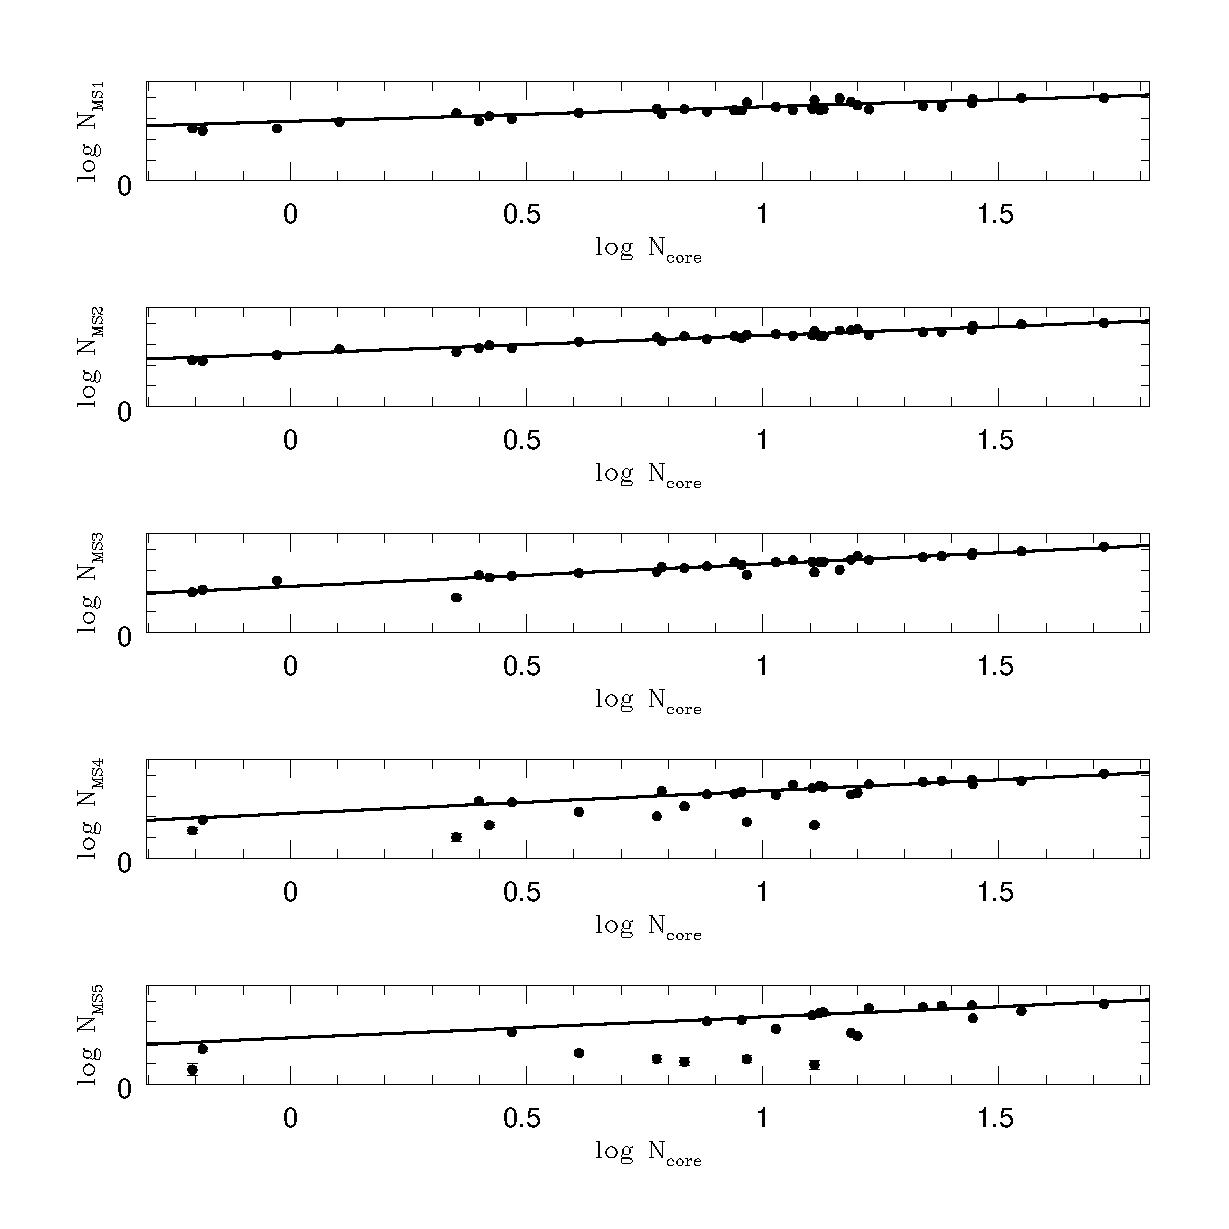
\includegraphics[scale=0.5]{Chapter-6/Ncore_vs_Nms_rc_new.ps}
\caption[Logarithm of the number of
stars belonging to each mass bin as a function of the
logarithm of the total number of stars spanning all five mass
bins in the core]{The logarithm of the number of
stars belonging to each mass bin as a function of the
logarithm of the total number of stars spanning all five mass
bins in the core.  MS1 corresponds to the mass range 0.65 - 0.75 M$_{\odot}$, MS2
to 0.55 - 0.65 M$_{\odot}$, MS3 to 0.45 - 0.55 M$_{\odot}$, MS4 to
0.35 - 0.45 M$_{\odot}$, and MS5 to 0.25 - 0.35 M$_{\odot}$.  Lines of
best fit are shown for each mass bin. 
\label{fig:Ncore_vs_Nms_rc}}
\end{center}
\end{figure}

\begin{figure} [!h]
  \begin{center}
 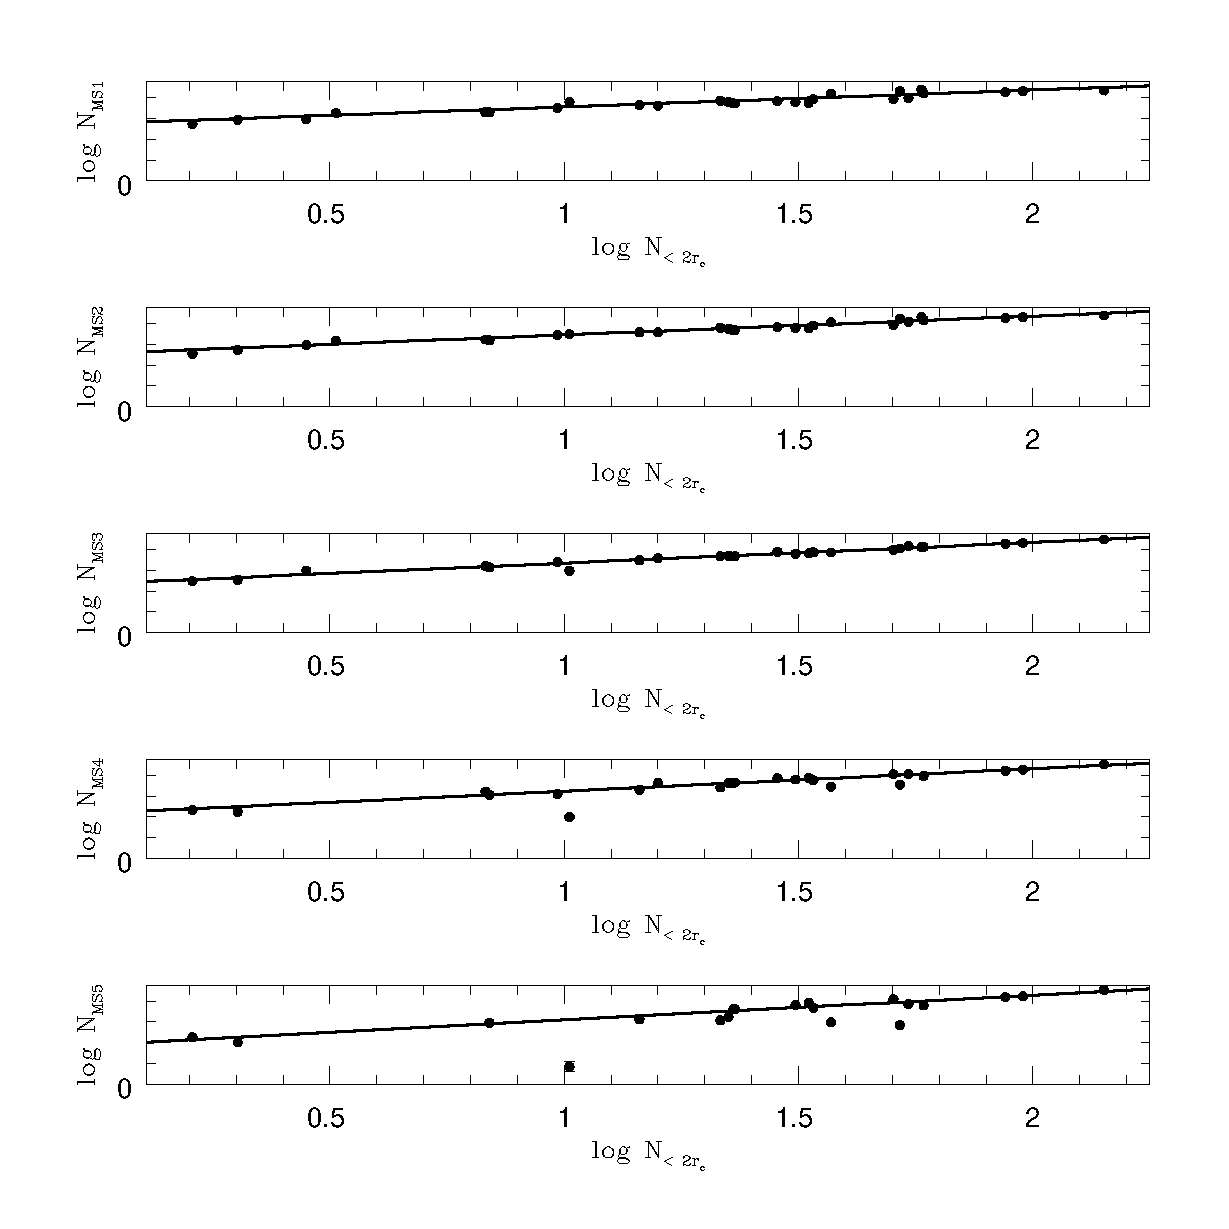
\includegraphics[scale=0.5]{Chapter-6/Ncore_vs_Nms_2rc_new.ps}
\caption[Logarithm of the number of
stars belonging to each mass bin as a function of the
logarithm of the total number of stars spanning all five mass
bins within two core radii from the cluster centre]{The logarithm of the number of
stars belonging to each mass bin as a function of the
logarithm of the total number of stars spanning all five mass
bins within two core radii from the cluster centre.  The mass bins are
the same as in Figure~\ref{fig:Ncore_vs_Nms_rc}.
%MS1 corresponds
%to the mass range 0.65 - 0.75 M$_{\odot}$, MS2
%to 0.55 - 0.65 M$_{\odot}$, MS3 to 0.45 - 0.55 M$_{\odot}$, MS4 to
%0.35 - 0.45 M$_{\odot}$, and MS5 to 0.25 - 0.35 M$_{\odot}$.  Lines of
%best fit are shown for each mass bin.
\label{fig:Ncore_vs_Nms_2rc}}
\end{center}
\end{figure}

\begin{figure} [!h]
  \begin{center}
 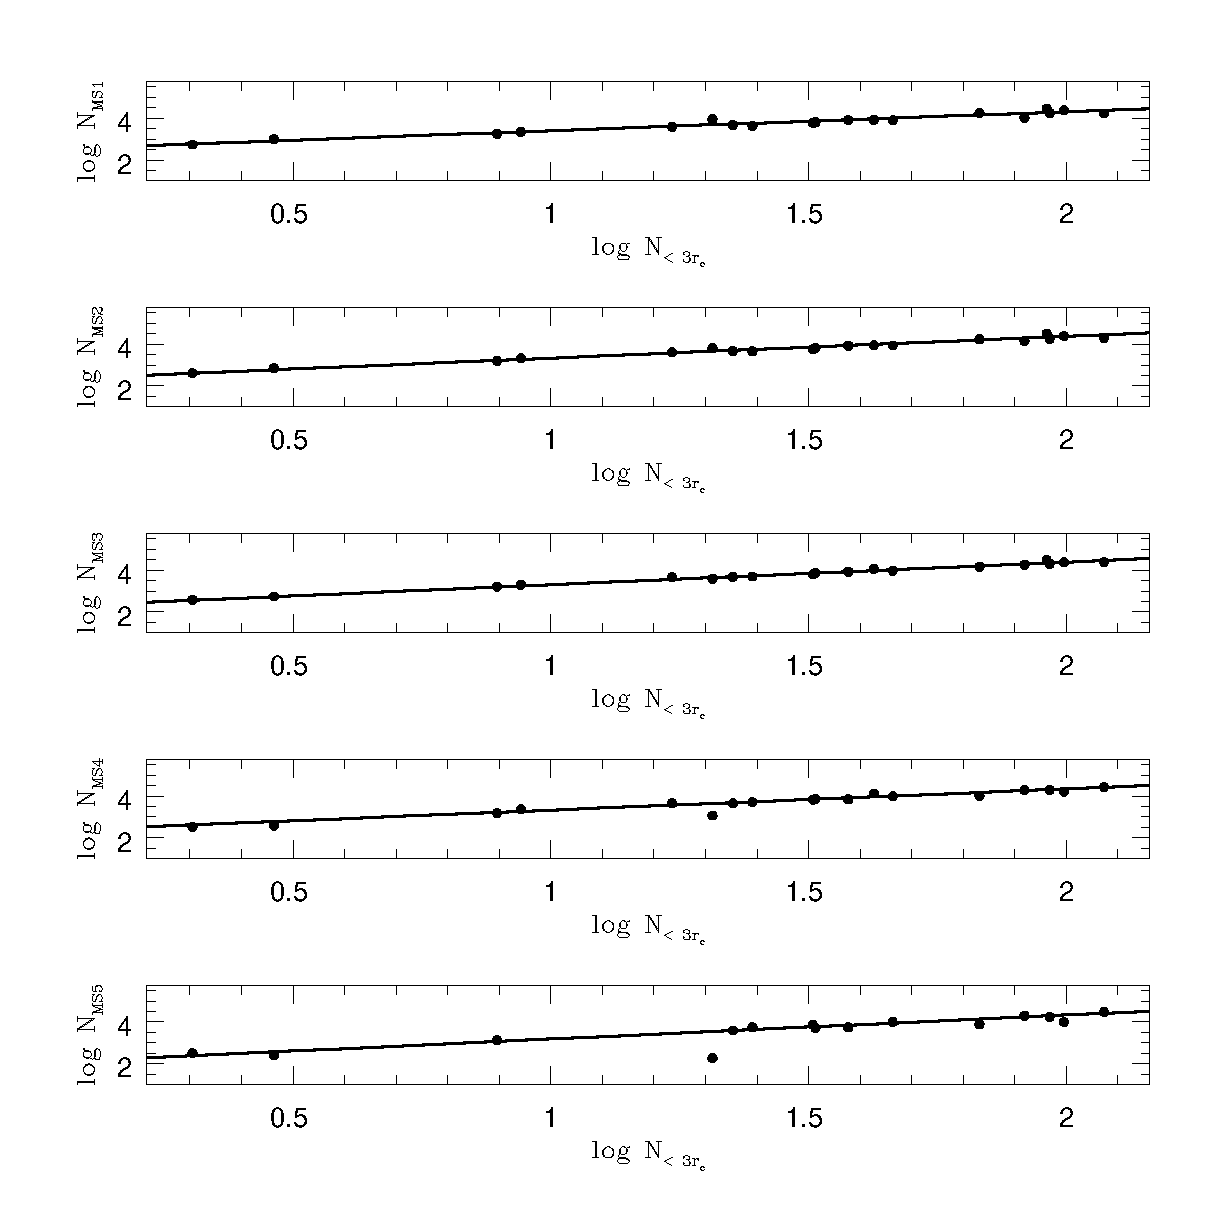
\includegraphics[scale=0.5]{Chapter-6/Ncore_vs_Nms_3rc_new.ps}
 \caption[Logarithm of the number of
 stars belonging to each mass bin as a function of the
 logarithm of the total number of stars spanning all five mass
 bins within three core radii from the cluster centre]{The logarithm of
  the number of
stars belonging to each mass bin as a function of the
logarithm of the total number of stars spanning all five mass
bins within three core radii from the cluster centre.  The mass bins are
the same as in Figure~\ref{fig:Ncore_vs_Nms_rc}.
%MS1 corresponds
%to the mass range 0.65 - 0.75 M$_{\odot}$, MS2
%to 0.55 - 0.65 M$_{\odot}$, MS3 to 0.45 - 0.55 M$_{\odot}$, MS4 to
%0.35 - 0.45 M$_{\odot}$, and MS5 to 0.25 - 0.35 M$_{\odot}$.  Lines of
%best fit are shown for each mass bin.
\label{fig:Ncore_vs_Nms_3rc}}
\end{center}
\end{figure}

%\begin{footnotesize}
\begin{sidewaystable}
\tiny
\centering
\caption{Lines of Best Fit for log N$_{MS}$ = (a $\pm$ $\Delta$a)log (N$_{tot}$/10$^3$) + (b $\pm$ $\Delta$b)
  \label{table:bestfit6}}
%\begin{tabular}{|l|p{4.5cm}|p{3.5cm}|p{3.5cm}|p{3.5cm}|p{3.5cm}|}
\begin{tabular}{|l|cccc|cccc|cccc|cccc|cccc|}
\hline
      &\multicolumn{4}{c|}{   MS1 (0.65-0.75 M$_{\odot}$)  }&\multicolumn{4}{c|}{   MS2 (0.55-0.65 M$_{\odot}$)  }&\multicolumn{4}{c|}{   MS3 (0.45-0.55 M$_{\odot}$)  }&\multicolumn{4}{c|}{   MS4 (0.35-0.45 M$_{\odot}$)  }&\multicolumn{4}{c|}{   MS5 (0.25-0.35 M$_{\odot}$)  }\\
%Circle      &   MS1 (0.65-0.75 M$_{\odot}$)  &   MS2 (0.55-0.65 M$_{\odot}$)  &   MS3 (0.45-0.55 M$_{\odot}$)  &   MS4 (0.35-0.45 M$_{\odot}$)  &   MS5 (0.25-0.35 M$_{\odot}$)  \\
\hline
Circle & a & $\Delta$a & b & $\Delta$b & a &$\Delta$a & b & $\Delta$b
& a & $\Delta$a & b & $\Delta$b & a & $\Delta$a & b & $\Delta$b & a &
$\Delta$a & b & $\Delta$b \\
%Circle       &          MS1 (0.65-0.75 M$_{\odot}$)             &           MS2 (0.55-0.65 M$_{\odot}$)            &              MS3 (0.45-0.55 M$_{\odot}$)            &            MS4 (0.35-0.45 M$_{\odot}$)           &           MS5 (0.25-0.35 M$_{\odot}$)            \\
\hline
$<$ r$_c$    & 0.70 & 0.07 & 2.85 & 0.09 & 0.86 & 0.05 & 2.56 & 0.05 & 1.08 & 0.05 & 2.22 & 0.07 & 1.08 & 0.09 & 2.17 & 0.12 & 1.00 & 0.20 & 2.24 & 0.25 \\
$<$ 2r$_c$   & 0.81 & 0.08 & 2.74 & 0.12 & 0.90 & 0.06 & 2.55 & 0.09 & 0.99 & 0.03 & 2.35 & 0.05 & 1.07 & 0.06 & 2.17 & 0.10 & 1.19 & 0.10 & 1.91 & 0.18 \\
$<$ 3r$_c$   & 0.91 & 0.12 & 2.50 & 0.19 & 1.04 & 0.11 & 2.30 & 0.17 & 1.08 & 0.08 & 2.23 & 0.12 & 1.02 & 0.05 & 2.31 & 0.10 & 1.15 & 0.10 & 2.04 & 0.16 \\
%
%$<$ r$_c$    & log(N$_{MS1}$) = (0.70 $\pm$ 0.07)log(N$_{tot}$/10$^3$) + (2.85 $\pm$ 0.09)  &    log(N$_{MS2}$) = (0.86 $\pm$ 0.05)log(N$_{tot}$/10$^3$) + (2.56 $\pm$ 0.05)    & log(N$_{MS3}$) = (1.08 $\pm$ 0.05)log(N$_{tot}$/10$^3$) + (2.22 $\pm$ 0.07)   & log(N$_{MS4}$) = (1.08 $\pm$ 0.09)log(N$_{tot}$/10$^3$) + (2.17 $\pm$ 0.12)  & log(N$_{MS5}$) = (1.00 $\pm$ 0.20)log(N$_{tot}$/10$^3$) + (2.24 $\pm$ 0.25)  \\
%$<$ 2r$_c$   & log(N$_{MS1}$) = (0.81 $\pm$ 0.08)log(N$_{tot}$/10$^3$) + (2.74 $\pm$ 0.12)  &    log(N$_{MS2}$) = (0.90 $\pm$ 0.06)log(N$_{tot}$/10$^3$) + (2.55 $\pm$ 0.09)    & log(N$_{MS3}$) = (0.99 $\pm$ 0.03)log(N$_{tot}$/10$^3$) + (2.35 $\pm$ 0.05)   & log(N$_{MS4}$) = (1.07 $\pm$ 0.06)log(N$_{tot}$/10$^3$) + (2.17 $\pm$ 0.10)  & log(N$_{MS5}$) = (1.19 $\pm$ 0.10)log(N$_{tot}$/10$^3$) + (1.91 $\pm$ 0.18)  \\
%$<$ 3r$_c$   & log(N$_{MS1}$) = (0.91 $\pm$ 0.12)log(N$_{tot}$/10$^3$) + (2.50 $\pm$ 0.19)  &    log(N$_{MS2}$) = (1.04 $\pm$ 0.11)log(N$_{tot}$/10$^3$) + (2.30 $\pm$ 0.17)    & log(N$_{MS3}$) = (1.08 $\pm$ 0.08)log(N$_{tot}$/10$^3$) + (2.23 $\pm$ 0.12)   & log(N$_{MS4}$) = (1.02 $\pm$ 0.05)log(N$_{tot}$/10$^3$) + (2.31 $\pm$ 0.10)  & log(N$_{MS5}$) = (1.15 $\pm$ 0.10)log(N$_{tot}$/10$^3$) + (2.04 $\pm$ 0.16)  \\
\hline
\end{tabular}
\end{sidewaystable}

As shown in Table~\ref{table:bestfit6}, the slopes tend to
systematically increase 
with decreasing mass bin.  For the comparison within two core radii
(shown in Figure~\ref{fig:Ncore_vs_Nms_2rc}), 
this trend applies to all mass bins.  For the comparisons within the core
and within three core radii (shown in Figure~\ref{fig:Ncore_vs_Nms_rc}
and Figure~\ref{fig:Ncore_vs_Nms_3rc}, respectively), however, only
the highest three mass bins (MS1, MS2, and MS3) 
follow this trend of increasing slope with decreasing mass bin.  After
the third mass bin, the slopes for the lowest two mass bins remain
about the same.  Note, however, that the uncertainties on the slopes
and y-intercepts are also higher for the lowest mass bins (MS4 and MS5).  
%
%For the most part, the slopes for each mass bin are consistent with their
%adjacent bins to within one standard deviation.  This is particularly
%true for the lowest two mass bins (MS4 and MS5) for which the
%uncertainties are typically the largest.  
This is
likely to be due to the fact that the photometric errors are the
highest at these dim magnitudes, however they remain at most $\sim$
10\% of the width in magnitude of their corresponding mass bins.  The
completeness corrections are also the largest for MS4 and MS5,
and this also introduces additional uncertainty.  Although we have
taken the appropriate measures, it
is important that these effects be properly quantified in order to reliably
use our technique to constrain the degree of universality of the IMF.
We will return to this in Section~\ref{discussion6}.  

On the other hand, when we consider only the largest three mass bins
(MS1, MS2, and MS3) for which 
the photometric errors and level of incompleteness are the lowest, the
difference in slopes and y-intercepts between adjacent mass bins can
differ at better than the $2-\sigma$ confidence level.  Moreover, if we
compare non-adjacent mass bins, then this trend is typically
significant at the $3-\sigma$ confidence level.  In order to improve
upon these statistics, we have also calculated reduced chi-squared
values with added intrinsic dispersion for the relations for each mass
bin.  That is, for each mass bin we added a constant term to the uncertainty for each
data point, found the value that yielded a reduced chi-squared of one,
and looked at the subsequent effects on the uncertainties for the
line of best-fit.  Based on this, we appear to be slightly over-estimating the
uncertainties for the MS1, MS2 and MS3 mass bins using our bootstrap
approach, and slightly under-estimating them for the MS4 and MS5
bins.  This suggests that the slopes and y-intercepts differ at nearly
the $2-\sigma$ confidence level for the MS1, MS2 and MS3 mass bins,
but are consistent to within one standard deviation for the MS4 and
MS5 bins.  We conclude that our results are the most reliable (at nearly the
$2-\sigma$ confidence level) in the mass range 0.45-0.75 M$_{\odot}$. 

The change in the distribution of stellar masses as a function of the
total cluster mass can be illustrated using pie charts, as shown in
Figure~\ref{fig:pie_charts}.  Using the slopes and y-intercepts
provided in Table~\ref{table:bestfit6} for the comparison within two core
radii, we have generated pie charts for three total numbers of stars
(spanning all five mass bins), namely N$_{tot}$ = 10$^3$, 10$^4$,
10$^5$.  As is clear, low-mass stars are preferentially depleted, and
this effect becomes increasingly severe with decreasing total cluster
mass (or, equivalently, increasing dynamical age).  From right to
left, what the pie charts are showing are the mass
functions of progressively dynamically older clusters.  %We will
%return to this issue in Section~\ref{discussion6}.  
If this is indeed the cause of the observed depletion of low-mass
stars in low-mass clusters, we are effectively looking at the
evolution of the stellar mass function in time.   

\begin{figure} [!h]
  \begin{center}
 \includegraphics[scale=0.5]{Chapter-6/pie_charts.ps}
    \caption[Mass Functions in Pie Chart Form]{
      Stellar mass functions depicted in pie chart form.  The total
      area of each circle corresponds to the total number of stars
      spanning all five mass bins, and each pie slice shows the
      fraction of this total corresponding to each mass bin.  Each of
      these fractions was calculated using the weighted lines of
      best-fit provided in Table~\ref{table:bestfit6}.  From left to
      right, the total number of stars used to generate each pie chart
      was 10$^3$, 10$^4$, and 10$^5$.  Dark blue corresponds to MS1,
      red to MS2, green to MS3, purple to MS4, and light blue to MS5.
      From right to left, the pie charts effectively show the mass functions of
      progressively dynamically older clusters.
      \label{fig:pie_charts}}
    \end{center}
\end{figure}

\section{Summary \& Discussion} \label{discussion6}

In this chapter, we have obtained completeness-corrected stellar mass
functions in the range 0.25-0.75 M$_{\odot}$ for a sample of 33
globular clusters using data taken from the ACS Survey for Globular
Clusters.  We have presented a new technique to quantify
cluster-to-cluster variations in the observed stellar mass functions.  
We have shown how our method can be used to quantify the universality
of the IMF for a large sample of clusters and, when used in
conjunction with theoretical models for globular cluster evolution,
can be used to constrain the degree to which two-body relaxation has
modified the currently observed stellar mass functions from their 
primordial form.  To this end, we have
obtained weighted lines of best-fit by comparing the number of stars in five
different mass bins to the total number of stars spanning the
entire mass range within several circles centred on the cluster
centre.  

As shown in Table~\ref{table:bestfit6}, our results suggest that the slopes
for the lines of best-fit tend to systematically increase
with decreasing mass bin.  Assuming all of the clusters in our sample
were born with similar IMFs, this is precisely what we expect from
two-body relaxation.  That is, we expect low-mass stars to become
preferentially depleted via stellar evaporation, and we expect this
effect to be the most severe in low-mass clusters.  This trend is
clearly seen in the observations, as demonstrated in 
Figure~\ref{fig:pie_charts}.  Interestingly, the fraction of stars
belonging to each mass bin is remarkably constant for all mass bins at
the high-mass end of our sample.  The total masses of these clusters
are sufficiently high that their half-mass relaxation times are
comparable to their ages \citep[e.g.][]{harris96}.  Therefore, we
expect that the highest mass clusters in our sample should have
been relatively unaffected by stellar evaporation due to two-body
relaxation.  It follows that their current mass functions should be
relatively unchanged from their primordial values (ignoring the
effects of stellar evolution).  If true, our
results could suggest that the slope IMF in Equation~\ref{eqn:kroupa}
was consistent with zero in the
mass range 0.25-0.75 M$_{\odot}$ for all of the clusters in our
sample.  This would be inconsistent with a ``standard'' Kroupa IMF.  This
hypothesis can be tested by comparing the results of the 
observational analysis presented in this chapter to simulations of
globular cluster evolution.  These can be used to directly quantify
the effects of two-body relaxation on the expected slopes and
y-intercepts for each mass bin given any set of initial conditions and
IMFs.  By comparing the results of these simulations to the results of
our observational analysis, the set of initial conditions that
best reproduces the observations can be found.  This will tell us
about the precise functional form of the IMF for the clusters in our
sample, in addition to the degree of primordial mass segregation.

The uncertainties for the slopes and 
y-intercepts are sufficiently large that they are often consistent with
those of their adjacent mass bins to within one standard deviation.
However, when we consider only the largest three mass bins for which
the photometric errors and level of incompleteness are the lowest, the
difference in slopes and y-intercepts between adjacent mass bins can
differ at better than the $2-\sigma$ confidence level.  Moreover, the
trend of increasing slope with decreasing mass is typically
significant at the $3-\sigma$ confidence level if we compare
non-adjacent mass bins.  Based on this, we conclude that our results
are consistent with a universal IMF for the clusters in our sample,
and that the currently observed mass functions have primarily been 
modified by internal two-body relaxation.  Having said that, it is
important to note that a higher degree of primordial mass segregation
effectively acts
to increase the rate of dynamical evolution and therefore stellar
evaporation \citep[e.g.][]{heggie03}.  Consequently, our results could
also be consistent with a non-universal IMF that depends on the total
cluster mass, provided the degree of primordial mass segregation also
depends systematically on the total cluster mass.  We also wish to
point out here 
that the large uncertainties found for the slopes and y-intercepts,
particularly for the two lowest mass bins, are primarily due to the
relatively large photometric errors at these dim magnitudes and
incompleteness resulting from crowding.  Despite the high quality of
the data used in this study, these issues are currently unavoidable
given the nature of the observations.  This will be a key challenge
for future studies to resolve, however the method we have presented
in this chapter offers a robust means of performing future analyses.

In terms of addressing the \textit{degree} of universality of the IMF,
our technique offers a considerable advantage over the standard
power-law and log-normal forms used to characterize the stellar mass
function shown in Equation~\ref{eqn:kroupa} and
Equation~\ref{eqn:miller}.  This is the case when comparing the mass
functions of a large sample of clusters.  The reason for this is that
our method
segments the mass function into mass bins, which characterizes
cluster-to-cluster differences in the stellar mass function for each
mass bin individually (i.e. as a function of stellar mass).  This
is done using the slopes and y-intercepts of the
relations found by correlating the number of stars in each mass bin
with the total number of stars spanning all mass bins.  Conversely,
standard Kroupa or Chabrier mass functions quantify the mass function
much more globally via functional fits to the data over considerably
larger mass ranges.  Of course, the standard forms
remain as useful as ever for characterizing the mass functions of
individual clusters, whereas our method is not appropriate for
this purpose.  That being
said, it is worth stating here that our results 
are consistent with those of \citet{demarchi10}, who fit a tapered
power-law distribution function with an exponential truncation to the
stellar mass functions of a sample of 30 clusters containing both
young and old members. 

There are several possible sources of additional uncertainty that
could have affected our analysis.  For 
instance, we have not yet considered the role played by binaries.
These tend to be unresolved in GCs, usually appearing as single
objects located above the MS in the 
cluster CMD.  Therefore, some of the objects in each mass bin are in
fact binaries masquerading as single stars.  Typical binary fractions
in Milky Way GCs are thought to be on the order of a few to a few tens
of a percent \citep[e.g.][]{rubenstein97, cool02, sollima08,
  davis08}.  This suggests that a non-negligible number of binaries
could often be included in our number counts for each mass bin.
However, there is no reason not to expect that binaries will
contribute to each mass bin in 
roughly equal proportions.  If the fraction of binaries is the same in
all mass bins, then the presence of binaries should not have
significantly affected the slopes.  Although they will have
affected the y-intercepts, this effect should not cause them to deviate
from within the uncertainties and 
should not have affected the interpretation of our results.  On the 
other hand, some observational evidence suggests that
the binary fraction could be inversely proportional to the total
cluster mass \citep[e.g.][]{sollima08, milone08, knigge09}.  It is not
clear how this might have affected our results since we do not know
how each mass bin should be affected.  It is our intent to address
this issue in a future study once binary fractions become available for
the majority of the clusters in our sample (Ata Sarajedini; private
communication).

Throughout our analysis, we have 
consistently compared two projected quantities.  Therefore, effects
related to projection should not have significantly affected
our results.  Moreover, these effects should become less severe upon
considering progressively larger circles, and we have performed 
our analysis for circles with three different sizes.  We note that
this could perhaps help to explain why 
the scatter in the lowest mass bins appears to become reduced for the
comparisons within two and three core radii (compared to the
comparison within one core radius), although it is not clear
why the agreement appears slightly better for the former comparison.  

Tidal effects from the Galaxy effectively act to reduce the time-scale
for two-body relaxation \citep[e.g.][]{heggie03}.  The same effect can also be had by
increasing the degree of primordial mass segregation
\citep[e.g.][]{spitzer87, portegieszwart01}.  Therefore, on average,
we would expect clusters with smaller Galactocentric radii and higher
initial concentrations to have experienced a higher degree of stellar
evaporation.  In an effort to quantify tidal effects from the Galaxy,
we performed several cuts in perigalacticon distance \citep{dinescu99,
  dinescu07} and re-performed our weighted lines of best-fit.  Despite
removing clusters from our sample with small perigalacticon distances
for which it is typically argued that tidal effects should be the most
severe \citep[e.g.][]{heggie03}, our slopes and 
y-intercepts, in addition to their uncertainties, remain more or less
unchanged.  This can be interpreted as rough evidence that tidal effects
from the Galaxy have not 
significantly affected our results.  It is much less clear which
clusters in our sample, if any, were born with high central 
concentrations.  Based on current observations, there is no
known reason not to expect a universal degree of primordial mass
segregation \citep[e.g.][]{portegieszwart10}.  If this was the case,
then our results could be interpreted as indicative of a
universal IMF for Milky Way globular clusters.  Unfortunately,
observational constraints for primordial 
binary populations are also lacking \citep[e.g.][]{mckee07}.  Binaries
play an important 
role in star cluster evolution by, for instance, providing an energy
source that serves to resist a cluster's tendency toward increasing 
its central density \citep{hut83}.  They are therefore an important consideration in
deciding the dynamical evolution of the stellar mass function, and
their role will need to be addressed in future studies.  

It is interesting and even surprising that, despite all of the
aforementioned factors 
expected to affect the dynamical evolution of globular clusters, we
observe relatively little scatter in the relations within two and
three core radii (Figure~\ref{fig:Ncore_vs_Nms_2rc} and
Figure~\ref{fig:Ncore_vs_Nms_3rc}).  Moreover, the slopes
systematically increase with decreasing mass bin.  Based on this, our
results are consistent with a single universal IMF for all of the
clusters in our sample that has been modified via internal two-body
relaxation by an amount determined by the total cluster mass.  
%and external effects such as tides from the Galaxy play a much less
%significant role (or that they are comparable in all clusters).
%Our results could also suggest that the initial cluster 
%conditions, including primordial mass segregation and the primordial
%binary fraction, are approximately universal for all Galactic GCs. 
%
%The small degree of scatter observed in
%Figure~\ref{fig:Ncore_vs_Nms_2rc} and
%Figure~\ref{fig:Ncore_vs_Nms_3rc} 
%Finally, our results provide compelling evidence of an approximately 
%universal IMF among all Galactic globular clusters.  
%The evidence in favour of a universal IMF is particularly compelling.
%Based on our results, this holds true for old Milky Way globular clusters
%having metallicities in the range [Fe/H] $\sim$ -(0.37 - 2.28)
%\citep{dotter10}.  
This is a new result given 
the old ages and therefore low metallicities ([Fe/H] $\sim$ -2.28 -
(-0.37)) of the clusters that comprise our sample.  However, the  
exact form of the IMF required to reproduce the current observations is
still not clear, nor is the role of primordial mass segregation.  To
what degree have low-mass clusters been depleted of 
their low-mass stars?  What combination of IMFs, Galactocentric
radii, initial concentrations and primordial binary fractions 
should evolve dynamically to best reproduce the currently observed
mass functions?  These questions can only be answered using 
simulations of globular cluster evolution that explore a range of
initial conditions and IMFs.  Our observational analysis of
the ACS data is ideally suited for comparison to these types of
models.  This would allow us to constrain the precise shape of the IMF
in the mass and metallicity range of interest, as well as to learn about
primordial mass segregation.  This will be the focus of a forthcoming
study. 

%
%PHOTOMETRIC ERRORS AND COMPLETENESS - both worse for dim, low-mass
%stars in the lowest two mass bins, hence the higher uncertainties.

\section*{Acknowledgments}

We would like to thank Ata Sarajedini, Aaron Dotter and Roger Cohen
for providing the data on which this study is based and for their
extensive support in its analysis.  We would also like to thank Evert
Glebbeek for useful discussions.  This research has been
supported by NSERC and OGS.

%\chapterbib

\begin{thebibliography}{99}

\bibitem[\protect\citeauthoryear{Anderson et al.}{2008}]{anderson08}
  Anderson J.,  Sarajedini A., Bedin L. R., King I. R., Piotto G.,
  Reid I. N., Siegel M., Majewski S. R., Paust N. E. Q., Aparicio A.,
  Milone A. P., Chaboyer B., Rosenberg A. 2008, AJ, 135, 2055
\bibitem[\protect\citeauthoryear{Bonnell, Larson \&
    Zinnecker}{2007}]{bonnell07} Bonnell I. A., Larson R. B.,
  Zinnecker H. 2007, Protostars and Planets V, 149 
  Elmegreen B. G. 1999, ApJ, 527, 266
\bibitem[\protect\citeauthoryear{Chabrier}{2005}]{chabrier05} Chabrier
  G. 2005, ASSL Vol. 327: The Initial Mass Function 50 Years Later, 41
\bibitem[\protect\citeauthoryear{Cool et al.}{2002}]{cool02} Cool
  A. M., Bolton
  A. S. 2002, in ASP Conference Series 263, Stellar Collisions,
  Mergers and their Consequences, ed. M. M. Shara (San Francisco:
  ASP), 163
\bibitem[\protect\citeauthoryear{Da Costa}{1982}]{dacosta82} Da Costa
  G. S. 1982, AJ, 87, 990
\bibitem[\protect\citeauthoryear{Davis et al.}{2008}]{davis08}
  Davis D. S., Richer H. B., Anderson J., Brewer J., Hurley J.,
  Kalirai J. S., Rich R. M., Stetson P. B. 2008, AJ, 135, 2155
\bibitem[\protect\citeauthoryear{Dinescu, Girard \& van
    Altena}{1999}]{dinescu99}
  Dinescu D. I., Girard T. M., van Altena W. F. 1999, AJ, 117, 1792
\bibitem[\protect\citeauthoryear{Casetti-Dinescu et al.}{2007}]{dinescu07}
  Casetti-Dinescu D. I., Girard T. M., Herrera D., van Altena W. F.,
  Lopez C. E., Castillo D. J. 2007, AJ, 134, 195
\bibitem[\protect\citeauthoryear{De Angeli et al.}{2005}]{deangeli05}
  De Angeli F., Piotto G., Cassisi S., Busso G., Recio-Blanco A.,
  Salaris M., Aparicio A., Rosenberg A. 2005, AJ, 130, 116
\bibitem[\protect\citeauthoryear{De Marchi, Paresce \& Portegies
    Zwart}{2010}]{demarchi10} De Marchi G., Paresce F., Portegies
  Zwart S. 2010, ApJ, 718, 105
\bibitem[\protect\citeauthoryear{Dotter et al.}{2007}]{dotter07}
  Dotter A., Chaboyer B., Jevremovic D., Baron E., Ferguson J. W.,
  Sarajedini A., Anderson J. 2007, AJ, 134, 376
\bibitem[\protect\citeauthoryear{Dotter et al.}{2010}]{dotter10}
  Dotter, A., Sarajedini A., Anderson J., Aparicio A., Bedin L. R.,
  Chaboyer B., Majewski S., Marin-Franch A., Milone A., Paust N.,
  Piotto G., Reid  N., Rosenberg A., Siegel M. 2010, ApJ, 708, 698
\bibitem[\protect\citeauthoryear{Elmegreen}{1999}]{elmegreen99}
  Elmegreen B. G. 1999, ApJ, 527, 266
\bibitem[\protect\citeauthoryear{Elmegreen}{2001}]{elmegreen01}
  Elmegreen B. G. 2001, ASP Conference Series 243: From Darkness to Light:
  Origin and Evolution of Young Stellar Clusters, 243, 255
\bibitem[\protect\citeauthoryear{Gieles et al.}{2010}]{gieles10}
  Gieles M., Baumgardt H., Heggie D., Lamers H. 2010, MNRAS, 408, L16
\bibitem[\protect\citeauthoryear{Gieles, Heggie \&
    Zhao}{2011}]{gieles11} Gieles M., Heggie D., Zhao H. 2011, MNRAS,
  accepted 
\bibitem[\protect\citeauthoryear{Goldsbury et al.}{2010}]{goldsbury10}
  Goldsbury R., Richer H. B., Anderson J., Dotter A., Sarajedini A.,
  Woodley K. 2010, AJ, 140, 1830
\bibitem[\protect\citeauthoryear{Grenier, Casandijan \&
    Terrier}{2005}]{grenier05} Grenier I. A., Casandjian J. M.,
  Terrier R. 2005, Science, 307, 1292
\bibitem[\protect\citeauthoryear{Harris}{1996, 2010 update}]{harris96}
  Harris, W. E. 1996, AJ, 112, 1487 (2010 update)
\bibitem[\protect\citeauthoryear{Heggie \& Hut}{2003}]{heggie03}
  Heggie D. C., Hut P. 2003, The Gravitational Million-Body Problem:
  A Multidisciplinary Approach to Star Cluster Dynamics (Cambridge:
  Cambridge University Press)
\bibitem[\protect\citeauthoryear{Henon}{1960}]{henon60} Henon M. 1960,
  Annales d'Astrophysique, 23, 668
\bibitem[\protect\citeauthoryear{Henon}{1973}]{henon73} Henon
  M. 1973, Dynamical Structure and Evolution of Dense Stellar Systems,
  ed. L. Martinet \& M. Mayor (Geneva Obs.)
\bibitem[\protect\citeauthoryear{Hurley et al.}{2005}]{hurley05}
  Hurley, J. R., Pols, O. R., Aarseth, S. J. \& Tout, C. A. 2005,
  MNRAS, 363, 293
\bibitem[\protect\citeauthoryear{Hut}{1983}]{hut83} Hut P. 1983, ApJ,
  272, 29
\bibitem[\protect\citeauthoryear{Knigge, Leigh \&
    Sills}{2009}]{knigge09} Knigge C., Leigh
  N., Sills A. 2009, Nature, 457, 288
\bibitem[\protect\citeauthoryear{Kroupa}{2001}]{kroupa01} Kroupa
  P. 2001, MNRAS, 322, 231
\bibitem[\protect\citeauthoryear{Lada}{1985}]{lada85} Lada C. J. 1985,
  ARA\&A, 23, 267
\bibitem[\protect\citeauthoryear{Lada \& Lada}{1995}]{lada95} Lada
  E. A., Lada C. J. 1995, AJ, 109, 1682
\bibitem[\protect\citeauthoryear{Lada \& Lada}{2003}]{lada03} Lada
  C. J., Lada E. A. 2003, ARA\&A, 41, 57
\bibitem[\protect\citeauthoryear{Lada, Alves \&
    Lombardi}{2007}]{lada07} Lada C. J., Alves J. F., Lombardi
  M. 2007, Protostars and Planets V, 3
\bibitem[\protect\citeauthoryear{McKee \& Ostriker}{2007}]{mckee07}
  McKee C. F., Ostriker E. C. 2007, ARA\&A, 45, 565
\bibitem[\protect\citeauthoryear{Miller \& Scalo}{1979}]{miller79}
  Miller G. E., Scalo J. M. 1979, ApJS, 41, 513
\bibitem[\protect\citeauthoryear{Milone et al.}{2008}]{milone08}
  Milone A. P., Piotto G., Bedin L. R., Sarajedini A. 2008, MmSAI, 79,
  623
\bibitem[\protect\citeauthoryear{Murray}{2009}]{murray09} Murray
  N. 2009, ApJ, 691, 946
\bibitem[\protect\citeauthoryear{Portegies Zwart et
    al.}{2001}]{portegieszwart01} Portegies Zwart S. F., McMillan
  S. L. W., Hut P., Makino J. 2001, MNRAS, 321, 199
\bibitem[\protect\citeauthoryear{Portegies Zwart, McMillan \&
    Gieles}{2010}]{portegieszwart10} Portegies Zwart S. F., McMillan
  S. L. W., Gieles M. 2010, ARA\&A, 48, 431
\bibitem[\protect\citeauthoryear{Rubenstein \&
    Bailyn}{1997}]{rubenstein97} Rubenstein E. P., Bailyn C. D. 1997,
  ApJ, 474, 701
\bibitem[\protect\citeauthoryear{Sarajedini et
    al.}{2007}]{sarajedini07}
  Sarajedini A., Bedin L. R., Chaboyer B., Dotter  A., Siegel M.,
  Anderson J., Aparicio A., King I., Majewski S., Marin-Franch A.,
  Piotto G., Reid  I. N., Rosenberg A., Steven M. 2007, AJ, 133, 1658
\bibitem[\protect\citeauthoryear{Scalo}{1998}]{scalo98} Scalo J. 1998,
  ASP Conference Series 142: The Stellar Initial Mass Function (38th
  Herstmonceux Conference), 142, 201
\bibitem[\protect\citeauthoryear{Sollima et al.}{2007}]{sollima07}
  Sollima A., Beccari G., Ferraro F. R., Fusi Pecci F., Sarajedini
  A. 2008, MNRAS, 380, 781
\bibitem[\protect\citeauthoryear{Sollima et al.}{2008}]{sollima08}
  Sollima A., Beccari G., Ferraro F. R., Fusi Pecci F., Sarajedini
  A. 2007, A\&A, 481, 701
\bibitem[\protect\citeauthoryear{Spitzer}{1987}]{spitzer87} Spitzer
  L. 1987, Dynamical Evolution of Globular Clusters (Princeton:
  Princeton University Press)
\bibitem[\protect\citeauthoryear{von Hippel \&
    Sarajedini}{1998}]{vonhippel98} von Hippel T., Sarajedini A. 1998,
  AJ, 116, 1789

\end{thebibliography}

%\bsp

%\label{lastpage}

%\end{document}

\pagestyle{fancy}
\headheight 20pt
\lhead{Ph.D. Thesis --- N. Leigh }
\rhead{McMaster - Physics \& Astronomy}
\chead{}
\lfoot{}
\cfoot{\thepage}
\rfoot{}
\renewcommand{\headrulewidth}{0.1pt}
\renewcommand{\footrulewidth}{0.1pt}

\chapter{Summary \& Future Work} \label{chapter7}
\thispagestyle{fancy}

%In this thesis, we have presented theoretical and statistical
%techniques broadly related to systems of dynamically-interacting
%particles.  We have applied these methods to observations of dense
%star clusters in order to study gravitational interactions between
%stars.  %These include both long- and short-range interactions, as well
%as encounters leading to direct collisions and mergers.  
%These
%processes have been described in detail in Chapter~\ref{chapter1}.
%They can be summarized as follows.  
%
%Within stellar communities, the life of a star can be dramatically
%impacted by its peers.  The interactions are typically peaceful and
%develop gradually over time.  However, violent encounters also occur
%and what can be thought of as a shoving match ensues.  The skirmish
%usually ends abruptly when one or more of the stars are forcefully
%propelled from the
%encounter.  From time to time, however, stars become entirely devoured
%by their opponents.  
%The effects of all of these interactions reverberate throughout
%clusters, stimulating their
%maturation.  Society evolves and adapts to accomodate the
%ever-changing demands its citizens impose upon it.
%
%Given the considerable evolution in our understanding of star clusters
%within the past few decades, what can be summarized as the study of
%stellar psychology has made considerable progress, particularly on the
%theoretical front.  That is, 
Within the last few decades, theoretical work has painted a
comprehensive picture for the 
various forms of gravitational interactions operating within star
clusters.  
And yet, direct observational confirmation that many of these processes
are actually occurring is still lacking.  %, and the 
%consequences of these different manifestations of stellar psychology.
The results presented in 
this thesis have connected several of these processes to real
observations of star clusters, in many cases for the first time.  This
has allowed us to directly link the observed
properties of several peculiar stellar populations to the physical
processes responsible for their origins.  Given the importance of star
clusters for star formation, this also represents a key step toward
re-constructing the history of our Galaxy.  
%Our results have advanced our understanding of stellar dynamics,
%stellar evolution and, in particular, the interplay that occurs
%between the two in dense star clusters. 

In Chapter~\ref{chapter2}, we have presented a new adaptation of the
mean free path approximation.  Our technique provides analytic
time-scales for the rate of close gravitational encounters between
single, binary and triple stars in dense star systems.  With it, we
showed that encounters involving triple stars occur more commonly than
any other type of dynamical interaction in at least some star
clusters, and that these could be the dominant dynamical production
mechanism for stellar mergers.  This is a new result with important
implications for both star cluster evolution and the formation of
several types of stellar exotica.  Our method
can be generalized for application to systems composed of several
different types of particles that evolve under the influence of any
force-mediated interactions.  For example, our technique is
well suited for application to collisions between atoms and dust
grains in the interstellar medium (ISM) \citep[e.g.][]{spitzer41a,
  spitzer41b, spitzer42}.  In this case, the relevant forces governing 
the dynamics are electromagnetic instead of gravitational, however the
general form adopted for the mean free path approximation remains the same.
Specifically, we must only replace the gravitationally-focused
collisional cross-sections with their charge-focused analogues.
Recent observations have provided 
estimates for the concentrations of the different constituents of the
ISM, in addition to their temperatures \citep[e.g.][]{delburgo03,
  kiss06}.  These data provide the required ingredients %for the
%application of our technique to the dynamics of the ISM.  This would yield
to obtain analytic estimates for the rates of collisions between
atoms, molecules, as well as both small and large dust grains in the
ISM, and would allow us to make
predictions for the evolution of their relative concentrations.  This
is an important step in the development of our understanding of dust
grain coagulation and, by extension, the initial phases of star
formation in dense molecular clouds \citep[e.g.][]{mckee07}, the
interaction of winds from
evolved stars with the surrounding ISM \citep[e.g.][]{glassgold96},
and planet formation in protoplanetary disks \citep[e.g.][]{absil10}.

In Chapter~\ref{chapter3}, we introduced a statistical technique to
compare the relative sizes of different populations of stars in a
large sample of star clusters.  %Our method was used to quantify
%how these distributions change with increasing radial distance from
%the cluster centre.  
We refined this technique in 
Chapter~\ref{chapter4}, and applied it to a large sample of clusters
collected using state-of-the-art observations.  Our results suggest
that dynamical effects do not significantly affect the relative sizes
of the different stellar populations.  This is the case for all
stellar populations above the main-sequence turn-off in the cluster
CMD.  Blue stragglers alone present a possible exception to this,
since we have identified a general trend in which more massive
clusters are home to proportionately smaller blue straggler
populations.  This provides compelling evidence in favour of a binary origin
for blue stragglers in even the dense 
cores of massive star clusters where direct collisions between stars are
expected to occur frequently \citep{knigge09}.  Although we have applied these
techniques to observations of dense star clusters throughout 
this thesis, they can be generalized for application to a number of
other studies related to population statistics.  For example, massive
elliptical galaxies have been identified in Galaxy Clusters and
Groups, and these could have formed from the mergers of smaller
galaxies.  Observational studies have now been 
performed that are allowing for the compilation of catalogues
providing population statistics for several different galaxy types in
a large number of Galaxy Clusters and Groups \citep[e.g.][]{abell58,
  abell89}.  Our technique is
well suited for application to these data, and would allow for a
systematic comparison between the relative population sizes of the
different galaxy types.  Among other things, this
would help to constrain the origins of massive elliptical galaxies in
Galaxy Clusters in
much the same way we have constrained the origins of BSs in globular
clusters.
% in a large sample of Galaxy Clusters and
%Groups.

%In Chapter~\ref{chapter3}, we have presented a new adaptation of the
%mean free path approximation.  Our technique provides analytic
%time-scales for the rate of close gravitational encounters between
%single, binary and triple stars in dense star systems.  With it, we
%showed that encounters involving triple stars occur more commonly than
%any other type of dynamical interaction in at least some star
%clusters, and that these could be the dominant dynamical production
%mechanism for stellar mergers.  This is a new result with important
%implications for both star cluster evolution and the formation of
%several types of stellar exotica.  Our method
%can be generalized for application to systems composed of several
%different types of particles that evolve under the influence of any
%force-mediated interactions.  For example, our technique is
%ideally suited for application to collisions between atoms and dust
%grains in the interstellar medium (ISM) \citep[e.g.][]{spitzer41a,
%  spitzer41b, spitzer42}.  Recent observations have provided
%estimates for the concentrations of the different consitituents of the
%ISM, in addition to their temperatures \citep[e.g.][]{delburgo03,
%  kiss06}.  These data provide the required ingredients for the
%application of our technique to the dynamics of the ISM.  This
%would yield analytic estimates for the rates of collisions between 
%atoms, molecules, as well as both small and large dust grains in the
%ISM, and would allow us to make
%predictions for the evolution of their relative concentrations.  This
%is an important step in the development of our understanding of dust
%grain coagulation and, by extension, the initial phases of star
%formation in dense molecular clouds \citep[e.g.][]{mckee07}, the
%interaction of winds from
%evolved stars with the surrounding ISM \citep[e.g.][]{glassgold96},
%and planet formation in protoplanetary disks \citep[e.g.][]{absil10}.
%
In Chapter~\ref{chapter5}, we present an analytic model for blue
straggler formation in globular clusters.  Our model considers the
production of blue stragglers throughout the entire cluster, and
tracks their accumulation in the core due to dynamical friction (or,
equivalently, two-body relaxation).  Our results support the
conclusion that blue stragglers are descended from binary stars, as
first reported in \citet{knigge09} using the technique presented in
Chapter~\ref{chapter3} and Chapter~\ref{chapter4}.  Our model is applicable to
studying the radial distributions of other stellar and binary
populations in globular clusters.  This is a sorely needed theoretical
tool that can be used to address a number of recent observational 
studies that reported peculiarities among the radial distributions of
several different stellar and binary populations
\citep[e.g.][]{rood73, fusipecci93, ferraro04, lanzoni07}.

Finally, in Chapter~\ref{chapter6}, we extend the statistical
technique introduced in 
Chapter~\ref{chapter3} and Chapter~\ref{chapter4} to include the
entire main-sequence.  By applying our method to the ACS data, we have
obtained the first quantitative constraints for the degree of
universality of the stellar initial mass function for a large sample
of star clusters spanning a wider range of masses and chemical
compositions than ever before considered.  Given the very old ages of
the clusters in our sample, our results have important
implications for our understanding of star formation in the early
Universe.  Our results are 
consistent with a remarkably universal IMF in old
massive star clusters, and are well suited for
comparison to theoretical simulations of globular cluster evolution.
This would provide a simple means of directly quantifying
the extent to which the stellar mass function has been modified from
its primordial form by two-body relaxation.  In future studies, this
will allow us to obtain the very first constraints for the precise
functional form of the IMF and the degree of
primordial mass segregation in a large sample of old star clusters.

The results presented in this thesis have significantly advanced our
understanding of stellar dynamics, 
stellar evolution and, in particular, the interplay that occurs
between the two in dense star clusters.
%The results presented in this thesis represent a significant step
%forward in our understanding of stellar evolution, stellar dynamics,
%and the various interactions they undergo in star clusters.  
But we
are not yet done.  Our results have raised several important questions
related to these topics and, by extension, the history of our Galaxy.
Once again, we are left asking:  Where do we go from here?   For
example, how else might we use observations of blue straggler
populations to learn about the dynamical histories of their host
clusters?  How can we use this information to constrain the
interactions that occur in clusters between stellar dynamics and
binary star evolution?  How do these interactions affect the
observed properties of their binary populations and the various types
of stellar exotica they are home to?  There is also the issue of the
universality of the stellar 
initial mass function.  What combination of initial concentrations and
mass functions should have evolved dynamically over the lifetimes of
star clusters to reproduce the currently observed mass functions?
What can this tell us about primordial mass segregation in massive
star clusters, and the exact form of the stellar IMF?  All of these
issues relate to the over-arching questions:  How do stars
form?; and:  How did the history of our Galaxy unfold?  %These
%questions offer crucial insight into our understanding of
%star formation, and the evolution of our Galaxy.  
The next few years promise to hold exciting advances in the search for
answers to these questions.
% is currently underway, and will be the focus of future studies. 




%The application of our techniques to observations of star clusters
%have brought us to the following conclusions.  
%GO OVER KEY RESULTS HERE.  WHAT DID WE FIND?
%
%WHY IS WHAT WE FOUND IMPORTANT?  BOTH FOR THE SPECIFIC FIELDS OF
%STELLAR DYNAMICS AND STELLAR EVOLUTION (AND THEIR INTERACTION), BUT
%ALSO FOR THE BROADER IMPLICATIONS?  HOW CAN OUR METHODS BE EXTENDED
%AND APPLIED TO OTHER ASTROPHYSICAL/PHYSICAL PROBLEMS AND SCENARIOS?
%WHAT SIMILAR POPULATION STATISTICS AND THEORETICAL
%PROCESSES/TECHNIQUES (E.G. MEAN-FREE PATH APPROXIMATION) DO THEY ALSO
%APPLY TO?
%
%THEN, DIRECTIONS FOR FUTURE WORK.  WHAT HAS OUR WORK TOLD US ABOUT
%WHERE TO GO FROM HERE?
%
%
%
%%%Let us return to the analogy between stars and people with which
%%%we began this thesis.  
%Within stellar communities, the life of a star can be dramatically
%impacted by its peers.  The interactions are typically peaceful and
%develop gradually over time.  However, violent encounters also occur
%and what can be thought of as a shoving match ensues.  The skirmish ends
%abruptly when one or more of the stars are forcefully propelled from the
%encounter.  Either that, or stars are devoured by their opponents.
%The effects of all of these interactions reverberate throughout
%clusters, stimulating their 
%maturation.  Society evolves and adapts to accomodate the
%ever-changing demands its citizens impose upon it.  
%
%Theoretical work has painted a comprehensive picture for the various
%forms of stellar psychology operating within clusters, and their
%consequences.  The results of 
%this thesis have connected several of these processes to real
%observations of star clusters, in many cases for the first time.
%Given the importance of star clusters for stellar birthing, this 
%is a key step toward re-constructing the history of our Galaxy.
%What's more, it has allowed us to directly link the observed
%properties of several peculiar stellar populations to the physical
%processes responsible for their origins.
%
% COME BACK TO ANALOGY BETWEEN STARS AND PEOPLE HERE.

%\chapterbib

\begin{thebibliography}{99}



\bibitem[\protect\citeauthoryear{Abell}{1958}]{abell58} Abell
  G. O. 1958, ApJS, 3, 211
\bibitem[\protect\citeauthoryear{Abell, Corwin \&
    Olowin}{1989}]{abell89} Abell G. O., Corwin Jr. H. G., Olowin
  R. P. 1989, ApJS, 70, 1
\bibitem[\protect\citeauthoryear{Absil \& Mawet}{2010}]{absil10} Absil
  O., Mawet D. 2010, A\&ARv, 18, 317
\bibitem[\protect\citeauthoryear{del Burgo et al.}{2003}]{delburgo03}
  del Burgo C., Laureijs R. J., Abraham P., Kiss Cs., 2003, MNRAS,
  346, 403
\bibitem[\protect\citeauthoryear{Ferraro et al.}{2004}]{ferraro04}
  Ferraro F. R., Beccari G., Rood, R. T., Bellazzini M., Sills A.,
  Sabbi E. 2004, ApJ, 603, 127
\bibitem[\protect\citeauthoryear{Fusi Pecci et al.}{1993}]{fusipecci93}
  Fusi Pecci F., Ferraro F. R., Bellazzini M., et al. 1993, AJ, 105,
  1145
\bibitem[\protect\citeauthoryear{Glassgold}{1996}]{glassgold96}
  Glassgold A. E. 1996, ARA\&A, 34, 241
\bibitem[\protect\citeauthoryear{Kiss et al.}{2008}]{kiss06} Kiss Cs.,
  Abraham P., Laureijs R. J., Moor A., Birkmann S. M. 2006, MNRAS,
  373, 1213
\bibitem[\protect\citeauthoryear{Knigge, Leigh \&
    Sills}{2009}]{knigge09} Knigge C., Leigh N., Sills A. 2009,
  Nature, 457, 288
\bibitem[\protect\citeauthoryear{Lanzoni et al.}{2007}]{lanzoni07}
  Lanzoni B., Dalessandro E., Perina S., Ferraro F. R., Rood R. T.,
  Sollima A. 2007, ApJ, 670, 1065
\bibitem[\protect\citeauthoryear{McKee \& Ostriker}{2007}]{mckee07}
  McKee C. F., Ostriker E. C. 2007, ARA\&A, 45, 565
\bibitem[\protect\citeauthoryear{Rood}{1973}]{rood73} Rood
  R. T. 1973, ApJ, 184, 815
\bibitem[\protect\citeauthoryear{Spitzer}{1941a}]{spitzer41a}
  Spitzer L. Jr. 1941, ApJ, 93, 369
\bibitem[\protect\citeauthoryear{Spitzer}{1941b}]{spitzer41b}
  Spitzer L. Jr. 1941, ApJ, 94, 232
\bibitem[\protect\citeauthoryear{Spitzer}{1942}]{spitzer42}
  Spitzer L. Jr. 1942, ApJ, 95, 329

\end{thebibliography}

%\bsp

\label{lastpage}

%%\end{singlespace}
\end{doublespace}


%%%%%%%%%%%%%%%%%%%%%%%%%%%%%%%%%%%%%%%%%%%%%%%%%%%%%%%%%%%%%%%
%Appendices
%%%%%%%%%%%%%%%%%%%%%%%%%%%%%%%%%%%%%%%%%%%%%%%%%%%%%%%%%%%%%%%
\appendix
\pagestyle{fancy}
\headheight 20pt
\lhead{PhD Thesis - N. Leigh }
\rhead{McMaster Physics and Astronomy}
\chead{}
\lfoot{}
\cfoot{\thepage}
\rfoot{}
\renewcommand{\headrulewidth}{0.1pt}
\renewcommand{\footrulewidth}{0.1pt}

\chapter{Appendix A} \label{Appendix-A} 
\thispagestyle{fancy} 

In this appendix, we present the collisional cross sections and
time-scales used in Chapter~\ref{chapter2}.  The
gravitationally-focused cross sections for 1+1,
1+2, 2+2, 1+3, 2+3 and 3+3 collisions can be found using
Equation 6 from \citet{leonard89}.  Neglecting the first term and
assuming that binary and triple stars are on average twice and three
times as massive as single stars, respectively, this gives for the
various collisional cross sections:
\begin{equation}
\label{eqn:cs-1+1}
\sigma_{1+1} \sim \frac{8{\pi}GmR}{v_{rel}^2},
\end{equation}
\begin{equation}
\label{eqn:cs-1+2}
\sigma_{1+2} \sim \frac{3{\pi}Gma_b}{v_{rel}^2},
\end{equation}
\begin{equation}
\label{eqn:cs-2+2}
\sigma_{2+2} \sim \frac{8{\pi}Gma_b}{v_{rel}^2},
\end{equation}
\begin{equation}
\label{eqn:cs-1+3}
\sigma_{1+3} \sim \frac{4{\pi}Gma_t}{v_{rel}^2},
\end{equation}
\begin{equation}
\label{eqn:cs-2+3}
\sigma_{2+3} \sim \frac{5{\pi}Gm(a_b + a_t)}{v_{rel}^2},
\end{equation}
\begin{equation}
\label{eqn:cs-3+3}
\sigma_{3+3} \sim \frac{12{\pi}Gma_t}{v_{rel}^2}.
\end{equation}
Values for the
pericenters assumed for the various types of encounters are shown in
Table~\ref{table:peri}, where $R$ is the average stellar
radius, $a_b$ is the average binary semi-major axis and $a_t$ is the
average semi-major axis of the outer orbits of triples.

\begin{table}
\centering
\caption{Pericenters Assumed for Each Encounter Type
  \label{table:peri}}
\begin{tabular}{lc}
\hline
Encounter Type & Pericenter \\
\hline
1+1 & $2R$ \\
1+2 & $a_b/2$ \\
1+3 & $a_t/2$ \\
2+2 & $a_b$ \\
2+3 & $(a_b + a_t)/2$ \\
3+3 & $a_t$ \\
\hline
\end{tabular}
\end{table}

In general, the time between each of the different encounter
types can be found using Equation~\ref{eqn:coll-rate} and
the gravitationally-focused cross sections for collision given
above.  Following the derivation of \citet{leonard89}, we can write
the encounter rate in the general form:
\begin{equation}
\label{eqn:coll-rate-gen}
\Gamma_{x+y} = N_xn_y{\sigma}_{x+y}v_{x+y},
\end{equation}
where $N_x$ and $n_y$ are the number and number density, respectively,
of single, binary or triple stars and $v_{x+y}$ is the relative
velocity at infinity between objects $x$ and $y$.  For instance, the
time between binary-binary encounters in the core of a cluster is
given by:
\begin{equation}
\begin{gathered}
\label{eqn:coll2+2}
\tau_{2+2} = 1.3 \times 10^7f_b^{-2} \Big(\frac{1
  pc}{r_c}\Big)^3\Big(\frac{10^3
  pc^{-3}}{n_0}\Big)^2 \\
\Big(\frac{v_{rms}}{5 km/s}\Big)\Big(\frac{0.5
  M_{\odot}}{<m>}\Big)\Big(\frac{1
  AU}{a_{b}} \Big) \mbox{ years}.
\end{gathered}
\end{equation}
Similarly, the times between 1+1, 1+2, 1+3, 2+3 and 3+3 encounters are
given by:
\begin{equation}
\begin{gathered}
\label{eqn:coll1+1}
\tau_{1+1} = 1.1 \times 10^{10}(1-f_b-f_t)^{-2}\Big(\frac{1 pc}{r_c}
\Big)^3 \Big(\frac{10^3 pc^{-3}}{n_0} \Big)^2 \\
\Big(\frac{v_{rms}}{5 km/s} \Big) \Big(\frac{0.5 M_{\odot}}{<m>} \Big)
\Big(\frac{0.5 R_{\odot}}{<R>} \Big)\mbox{ years},
\end{gathered}
\end{equation}
\begin{equation}
\begin{gathered}
\label{eqn:coll1+2}
\tau_{1+2} = 3.4 \times 10^7(1-f_b-f_t)^{-1}f_b^{-1} \Big(\frac{1
  pc}{r_c}
\Big)^3 \Big(\frac{10^3 pc^{-3}}{n_0} \Big)^2 \\
\Big(\frac{v_{rms}}{5
  km/s} \Big) \Big(\frac{0.5 M_{\odot}}{<m>} \Big) \Big(\frac{1
  AU}{a_{b}} \Big)\mbox{ years},
\end{gathered}
\end{equation}
\begin{equation}
\begin{gathered}
\label{eqn:coll1+3}
\tau_{1+3} = 2.6 \times 10^7(1-f_b-f_t)^{-1}f_t^{-1} \Big(\frac{1
  pc}{r_c}
\Big)^3 \Big(\frac{10^3 pc^{-3}}{n_0} \Big)^2 \\
\Big(\frac{v_{rms}}{5
  km/s} \Big) \Big(\frac{0.5 M_{\odot}}{<m>} \Big) \Big(\frac{1
  AU}{a_{t}} \Big)\mbox{ years},
\end{gathered}
\end{equation}
\begin{equation}
\begin{gathered}
\label{eqn:coll2+3}
\tau_{2+3} = 2.0 \times 10^7f_b^{-1}f_t^{-1} \Big(\frac{1 pc}{r_c}
\Big)^3 \Big(\frac{10^3 pc^{-3}}{n_0} \Big)^2 \\
\Big(\frac{v_{rms}}{5
  km/s} \Big) \Big(\frac{0.5 M_{\odot}}{<m>} \Big) \Big(\frac{1
  AU}{a_{b}+a_{t}} \Big)\mbox{ years},
\end{gathered}
\end{equation}
and
\begin{equation}
\begin{gathered}
\label{eqn:coll3+3}
\tau_{3+3} = 8.3 \times 10^6f_t^{-2} \Big(\frac{1 pc}{r_c}
\Big)^3 \Big(\frac{10^3 pc^{-3}}{n_0} \Big)^2 \\
\Big(\frac{v_{rms}}{5
  km/s} \Big) \Big(\frac{0.5 M_{\odot}}{<m>} \Big) \Big(\frac{1
  AU}{a_{t}} \Big)\mbox{ years}.
\end{gathered}
\end{equation}



\pagestyle{fancy}
\headheight 20pt
\lhead{PhD Thesis - N. Leigh }
\rhead{McMaster Physics and Astronomy}
\chead{}
\lfoot{}
\cfoot{\thepage}
\rfoot{}
\renewcommand{\headrulewidth}{0.1pt}
\renewcommand{\footrulewidth}{0.1pt}

\chapter{Appendix B} \label{Appendix-B}
\thispagestyle{fancy}

In this appendix, we present our selection criteria for BS, RGB, HB
and MSTO stars used in Chapter~\ref{chapter4}.  Our method is similar
to that described in \citet{leigh07},
and we have used this as a basis for the selection criteria presented
in this chapter.  First, we define a location for the MSTO in the
(F606W-F814W)-F814W plane using our isochrone fits.  The MSTO is
chosen to be the bluest point along the MS of each isochrone, which we
denote by ((V-I)$_{MSTO}$,I$_{MSTO}$).  In order to distinguish BSs
from MSTO stars, we impose the conditions:

\begin{equation}
\label{eqn:bs_msto1}
F814W \le m_1(F606W-F814W) + b_{11},
\end{equation}
where the slope of this line is $m_1 = -9$ and its y-intercept is
given by:
\begin{equation}
\label{eqn:b_11}
b_{11} = (I_{MSTO}-0.10)-m_1((V-I)_{MSTO}-0.10)
\end{equation}

Similarly, we distinguish BSs from HB stars by defining the following
additional boundaries:
\begin{eqnarray}
\label{bs_hb1}
F814W &\ge& m_1(F606W-F814W) + b_{12} \\
F814W &\ge& m_2(F606W-F814W) + b_{21} \\
F814W &\le& m_2(F606W-F814W) + b_{22} \\
F814W &\ge& m_{HB}(F606W-F814W) + b_{HB} \\
(F606W-F814W) &\ge& (V-I)_{HB} \\
F814W &\le& I_{MSTO},
\end{eqnarray}
where $m_2 = 6$, $m_{HB} = -1.5$ and $(V-I)_{HB} = (V-I)_{MSTO} -
0.4$.  We also define:
\begin{eqnarray}
\label{b_12}
b_{12} &=& (I_{MSTO}-0.55)-m_1((V-I)_{MSTO}-0.55) \\
b_{21} &=& (I_{MSTO}-0.80)-m_2((V-I)_{MSTO}+0.10) \\
b_{22} &=& (I_{MSTO}+0.30)-m_2((V-I)_{MSTO}-0.20),
\end{eqnarray}
and $b_{HB} = I_{HB} + 1.2$, where $I_{HB}$ roughly corresponds to the
mid-point of points that populate the HB and is chosen
by eye for each cluster so that our selection criteria best fits the
HB in all of the CMDs in our sample.

We apply a similar set of conditions to the RGB in order to select
stars belonging to this stellar population.  These boundary conditions
are:
\begin{eqnarray}
\label{rgb_1}
F814W &\ge& m_{HB}(F606W-F814W) + b_{HB} \\
F814W &\ge& m_{RGB}(F606W-F814W) + b_{31} \\
F814W &\le& m_{RGB}(F606W-F814W) + b_{32} \\
F814W &\le& I_{RGB},
\end{eqnarray}
where $m_{RGB} = -23$, $I_{RGB}$ is defined as the F814W magnitude
corresponding to a core helium mass of 0.08 M$_{\odot}$ and:
\begin{eqnarray}
\label{b_31_and_b_32}
b_{31} &=& (I_{MSTO}-0.60)-m_{RGB}((V-I)_{MSTO}+0.05) \\
b_{32} &=& (I_{MSTO}-0.60)-m_{RGB}((V-I)_{MSTO}+0.25)
\end{eqnarray}

Core helium-burning stars, which we refer to as HB stars, are selected
if they satisfy one of the following sets of criteria:
\begin{eqnarray}
\label{hb1}
F814W &\ge& m_{HB}(F606W-F814W) + (b_{HB}-1.0) \\
F814W &\le& m_{HB}(F606W-F814W) + b_{HB} \\
(F606W-F814W) &\le& (V-I)_{MSTO} + (V-I)_{HB},
\end{eqnarray}
\begin{eqnarray}
\label{hb2}
F814W &>& m_{HB}(F606W-F814W) + b_{HB} \\
F814W &\le& I_{MSTO} + 2.5 \\
(F606W-F814W) &<& (V-I)_{MSTO} - 0.4,
\end{eqnarray}
or
\begin{eqnarray}
\label{hb3}
F814W &<& m_1(F606W-F814W) + b_{12} \\
F814W &>& m_{HB}(F606W-F814W) + b_{HB} \\
(F606W-F814W) &\ge& (V-I)_{MSTO} - 0.4
\end{eqnarray}
We define $(V-I)_{HB}$ on a cluster-by-cluster basis in order to
ensure that we do not over- or under-count the number of HB stars.
This is because the precise value of (F606W-F814W) at which the HB
becomes the RGB varies from cluster-to-cluster.  In addition, the
precise location of the transition in the cluster CMD between HB
and EHB stars remains poorly understood.  To avoid this ambiguity, we
consider HB and EHB stars
together throughout our analysis, and collectively refer to all core
helium-burning stars as HB stars throughout this chapter.

Finally, MSTO stars are selected according to the following criteria:
\begin{eqnarray}
\label{msto_1}
F814W &>& I_{RGB} \\
F814W &>& m_1(F606W-F814W) + b_{11} \\
F814W &\le& (V-I)_{MSTO}
\end{eqnarray}



%%%%%%%%%%%%%%%%%%%%%%%%%%%%%%%%%%%%%%%%%%%%%%%%%%%%%%%%%%%%%%%
% ESM students need to include a Nontechnical Abstract as the %
% last appendix.                                              %
%%%%%%%%%%%%%%%%%%%%%%%%%%%%%%%%%%%%%%%%%%%%%%%%%%%%%%%%%%%%%%%
% This \include command should point to the file containing
% that abstract.
%\include{nontechnical-abstract}
%%%%%%%%%%%%%%%%%%%%%%%%%%%%%%%%%%%%%%%%%%%
% End of the \allowdisplaybreak command %
%%%%%%%%%%%%%%%%%%%%%%%%%%%%%%%%%%%%%%%%%%%



%%%%%%%%%%%%%%%%
% BIBLIOGRAPHY %
%%%%%%%%%%%%%%%% 
% You can use BibTeX or other bibliography facility for your
% bibliography. LaTeX's standard stuff is shown below. If you
% bibtex, then this section should look something like:
\begin{singlespace}
  
  \pagestyle{fancy}
  \headheight 20pt
  \lhead{Ph.D. Thesis - N. Leigh}
  \rhead{McMaster - Physics and Astronomy}
  \chead{}
  \lfoot{}
  \cfoot{\thepage}
  \rfoot{}
  \renewcommand{\headrulewidth}{0.1pt}
  \renewcommand{\footrulewidth}{0.1pt}
  \thispagestyle{fancy}
  
  \bibliography{myrefs}
% \bibliographystyle{ieeetr}
  \bibliographystyle{apj}
%  \bibliographystyle{plain}
  \nocite{*}
  
  \addcontentsline{toc}{chapter}{Bibliography}
  
  \thispagestyle{fancy}
  
\end{singlespace}


\end{document}
